\documentclass[11pt,          % font size: 11pt or 12pt
               phd,           % degree:    ms or phd
               onehalfspacing % spacing: onehalfspacing or doublespacing
               ]{ncsuthesis}

%%----------------------------------------------------------------------------%%
%%------------------------------ Import Packages -----------------------------%%
%%----------------------------------------------------------------------------%%

\usepackage{booktabs}  % professionally typeset tables
\usepackage{amsmath}%,amssymb,amsfonts}
\DeclareMathOperator{\sgn}{sgn}
\usepackage{textcomp}  % better copyright sign, among other things
\usepackage{xcolor}
\usepackage{lipsum}    % filler text
%% \usepackage{subfig}    % composite figures
\usepackage{subcaption}% should hopefully allow subfigures
\usepackage{listings}  % Allows code printing
%% \usepackage{color}
\usepackage{morefloats}
\usepackage{tabularx}
\def\tabularxcolumn#1{m{#1}}
\usepackage[flushleft]{threeparttable}
\usepackage{threeparttablex}
\usepackage{longtable}
\usepackage{mathtools}

\DeclarePairedDelimiter\abs{\lvert}{\rvert}%
\DeclarePairedDelimiter\norm{\lvert}{\rvert}%

\makeatletter
\let\oldabs\abs
\def\abs{\@ifstar{\oldabs}{\oldabs*}}
%
\let\oldnorm\norm
\def\norm{\@ifstar{\oldnorm}{\oldnorm*}}
\makeatother

\definecolor{codegreen}{rgb}{0,0.6,0}
\definecolor{codegray}{rgb}{0.5,0.5,0.5}
\definecolor{codepurple}{rgb}{0.58,0,0.82}
\definecolor{backcolour}{rgb}{0.95,0.95,0.92}

\lstdefinestyle{mystyle}{
    backgroundcolor=\color{backcolour},
    commentstyle=\color{codegreen},
    keywordstyle=\color{magenta},
    numberstyle=\tiny\color{codegray},
    stringstyle=\color{codepurple},
    basicstyle=\footnotesize,
    breakatwhitespace=false,
    breaklines=true,
    captionpos=b,
    keepspaces=true,
    numbers=left,
    numbersep=5pt,
    showspaces=false,
    showstringspaces=false,
    showtabs=false,
    tabsize=2
}

\lstset{style=mystyle}


%%ORTIZ PACKAGES


%%%%%%%%%%%%%%%%%%%%%%%%%%%%%%%%%%%%%%%%%%
%%%%%%%%%%% Old bibliography commands
%%%%%%%%%%%%%%%%%%%%%%%%%%%%%%%%%%%%%%%%%%5
%\usepackage[super,sort&compress,comma,square,authoryear]{natbib} %\cite command %Added by Ortiz

%use the following line with plainnat
%\usepackage[super,sort&compress,comma,square,numbers]{natbib} %\cite command %Added by Ortiz
%\usepackage{natbib}

%\usepackage[style=alphabetic,natbib=true,backend=bibtex
%sorting=nyt,firstinits=true,isbn=false,doi=false,url=false]{biblatex} %couldn't get backend=biber to work

%\usepackage{filecontents}

%\bibliography{Ortiz-thesis2}
%\bibliographystyle{plain}


%%%%%%%%%%%%%%%%%%%%%%%%%%%%%%%%%%%%%%%%%%
%%%%%%%%%%% Hack for alphanumeric bibliography
%%%%%%%%%%%%%%%%%%%%%%%%%%%%%%%%%%%%%%%%%%5
%% \RequirePackage[
%% 			style=alphabetic,%numeric-comp,%authoryear-comp,%
%% 			sorting=nyt,%ynt
%% 			hyperref=true, %
%% 			firstinits=true,%
%% 			backend=bibtex,
%% 			natbib=true,
%% 			url=false,
%% 			isbn=false,
%% 			maxnames=2, %for et al to be used
%% 			maxalphanames=1, %to avoid printing a + for every et al in the abbreviation
%% 			doi=false]{biblatex}


%% %needed to do et al after two names
%% %http://tex.stackexchange.com/questions/44048/use-et-al-in-biblatex-custom-style
%% \renewcommand*{\finalnamedelim}{\addspace\&\space}

%% %Simplify abbreviation (the default uses either one or two authors and it indicates et al with a +)
%% %The following five lines make it so that only the first author is used in the abbreviation
%% %http://tex.stackexchange.com/questions/27956/label-only-from-first-author
%% \renewcommand*{\labelalphaothers}{}
%%     \renewcommand*{\intitlepunct}{}
%%     \DefineBibliographyStrings{german}{in={}}
%%     \DefineBibliographyStrings{english}{in={}}
%%     \DeclareNameAlias{sortname}{last-first}
%%     \DeclareNameAlias{default}{last-first}

%% %\AtEveryCitekey{\ifciteseen{}{\defcounter{maxnames}{99}}} %authoryear
%% \DeclareFieldFormat[article,periodical]{volume}{\mkbibbold{#1}}
%% \makeatletter

%% \newrobustcmd*{\parentexttrack}[1]{%
%%   \begingroup
%%   \blx@blxinit
%%   \blx@setsfcodes
%%   \blx@bibopenparen#1\blx@bibcloseparen
%%   \endgroup}

%% \AtEveryCite{%
%%   \let\parentext=\parentexttrack%
%%   \let\bibopenparen=\bibopenbracket%
%%   \let\bibcloseparen=\bibclosebracket}

%% \makeatother
%% \renewcommand{\cite}[1]{\parencite{#1}}


%% \renewbibmacro{in:}{%
%%   \ifentrytype{article}{}{%
%%   \printtext{\bibstring{in}\intitlepunct}}}

%% \AtEveryBibitem{\clearfield{month}}

%% \AtEveryBibitem{\clearfield{language}}
%% %%%%%%%%%%%%%%%%%%%%%%%%%%%%%%%%%%%%%%%%%%%%%

%% \addbibresource{AlexLindsay-thesis.bib}

%%  \defbibheading{myheading}[BIBLIOGRAPHY]{
%%  \chapter*{#1}
%%  %\centerline{\bf{#1}}
%%  \markboth{#1}{#1}}

%\usepackage{amsmath,amssymb,amsfonts} %amssymb and amsfonts cannot be used in conjunction with mdput
%\usepackage{graphicx,subfig}% Include figure files
\usepackage{dcolumn}% Align table columns on decimal point
\usepackage{bm}% bold math
%\usepackage{hyperref}% add hypertext capabilities
%\usepackage{hypernat}% make hyperref and natbib work together
\usepackage{cancel}
%% \usepackage{verbatim}% multiline commenting
\usepackage{ifthen}
\usepackage{url}
\usepackage{sectsty}
\usepackage{balance}
%\usepackage{caption}
\usepackage{graphicx} %eps figures can be used instead
\makeatletter
\def\maxwidth#1{\ifdim\Gin@nat@width>#1 #1\else\Gin@nat@width\fi}
\makeatother
\usepackage{lastpage}
\usepackage[format=plain,justification=RaggedRight,singlelinecheck=false,font=small,labelfont=bf,labelsep=space]{caption}
\usepackage{fancyhdr}
\pagestyle{fancy}
\newcounter{magicrownumbers}
\newcommand\rownumber{\stepcounter{magicrownumbers}\arabic{magicrownumbers}}

%http://tex.stackexchange.com/questions/100817/error-when-using-bc-from-abbrevs-in-caption
%Getting BC
\usepackage{abbrevs}
\usepackage{etoolbox}
\robustify{\DateMark} % after having loaded abbrevs

\usepackage{units} %Needed to solve bug from citation Hydrodynamics in 21/2 dimensions
%see http://www.latex-community.org/viewtopic.php?f=5&t=989

\usepackage[sharp]{easylist} %used for brainstorming purposes
%\usepackage{mathabx} % used for \Asterisk for convolution %conflicts with \widering

%compile on single pass
%\usepackage[backend=biber,...]{biblatex}


%%%%%%%%%%%%
%%% Hack to make chapters start on odd pages
% http://tex.stackexchange.com/questions/73591/how-to-have-a-blank-even-page-before-every-chapter
%%%%%%%%%%%%
%\newcommand{\ensureoddstart}{\checkoddpage\ifoddpage\else\newpage\mbox{}\fi}
%\newcommand{\ensureoddstart}{}


%%%Fancy tables
%http://tex.stackexchange.com/questions/94032/fancy-tables-in-latex
%% \usepackage[table]{xcolor}
\usepackage{array,booktabs}
\usepackage{colortbl}
\newcolumntype{L}{@{}>{\kern\tabcolsep}l<{\kern\tabcolsep}}



%%%%%%%%%%
%%%%% Hack to allow more levels in outline
%%%%%%%%%%
%\setcounter{secnumdepth}{5}
%\setcounter{tocdepth}{5} %may violate ETD
%Usage http://pleasemakeanote.blogspot.com/2010/06/how-to-activate-subsubsubsection-in.html
%\section{} % level 1
%\subsection{} % level 2
%\subsubsection{} % level 3
%\paragraph{} % level 4 - equivalent to subsubsubsection
%\subparagraph{} % level 5

%http://tex.stackexchange.com/questions/60209/how-to-add-an-extra-level-of-sections-with-headings-below-subsubsection
\usepackage{titlesec}

\setcounter{secnumdepth}{4}

\titleformat{\paragraph}
{\normalfont\normalsize\bfseries}{\theparagraph}{1em}{}
\titlespacing*{\paragraph}
{0pt}{3.25ex plus 1ex minus .2ex}{1.5ex plus .2ex}

%%%%%%%%%%%%%%%%%%%%%%%%%%
%%%% Hack for containing figures within sections
%%%%%%%%%%%%%%%%%%%%%%%%%%%%
%http://ctan.org/pkg/placeins
\usepackage{placeins}
%De�fines a \FloatBar�rier com�mand, be�yond which floats may not pass; use�ful, for ex�am�ple, to en�sure all floats for a sec�tion ap�pear be�fore the next \sec�tion com�mand.

%%----------------------------------------------------------------------------%%
%%---------------------------- Formatting Options ----------------------------%%
%%----------------------------------------------------------------------------%%
%%

%% -------------------------------------------------------------------------- %%
%% Disposition format -- any titles, headings, section titles
%%  These formatting commands affect all headings, titles, headings,
%%  so sizing commands should not be used here.
%%  Formatting options to consider are
%%     +  \sffamily - sans serif fonts.  Dispositions are often typeset in
%%                    sans serif, so this is a good option.
%%     +  \rmfamily - serif fonts
%%     +  \bfseries - bold face
%\dispositionformat{\sffamily\bfseries}   % bold and sans serif
\dispositionformat{\bfseries}            % bold and serif

%% -------------------------------------------------------------------------- %%
%% Formatting for centered headings - Abstract, Dedication, etc. headings
%%  This is where one might put a sizing command.
%%  \MakeUppercase can be used to typeset all headings in uppercase.
\headingformat{\large\MakeUppercase}   % All letters uppercase
%% \headingformat{\large}                % Not all uppercase
%\headingformat{\Large\scshape}        % Small Caps, used with serif fonts.

%% Typographers recommend using a normal inter-word space after
%% sentences. TeX's default is to add an wider space, but \frenchspacing
%% gives a normal spacing. Comment out the following line if you prefer
%% wider spaces between sentences.
\frenchspacing


%% -------------------------------------------------------------------------- %%
%%  Optional packages
%%    A number of compatible packages to improve the look and feel of
%%    your document are available in the file optional.tex
%%    (For example, hyperlinks, fancy chapter headings, and fonts)
%% To use these options, uncomment the next line and see optional.tex
%%  Optional Packages to consider.   These packages are compatible with
%%    ncsuthesis.  

%% -------------------------------------------------------------------------- %%
%% Fancy chapter headings
%%  available options: Sonny, Lenny, Glenn, Conny, Rejne, Bjarne
%\usepackage[Sonny]{fncychap}
\usepackage[Rejne]{fncychap}

%%----------------------------------------------------------------------------%%
%% Hyperref package creates PDF metadata and hyperlinks in Table of Contents
%%  and citations.  Based on feedback from the NCSU thesis editor, 
%%  the links are not visually distinct from normal text (i.e. no change
%%  in color or extra boxes).
\usepackage[
  pdfauthor={Carlos Pompeyo Ortiz},
  pdftitle={Rigidity of Microsphere Heaps},
  pdfcreator={pdftex},
  pdfsubject={NC State ETD Thesis},
  pdfkeywords={microfluidics, hard sphere, jamming, suspension, rigidity, friction, microscopy},
  colorlinks=true,
  linkcolor=black,
  citecolor=black,
  filecolor=black,
  urlcolor=black,
]{hyperref}


%% -------------------------------------------------------------------------- %%
%% Microtype - If you use pdfTeX to compile your thesis, you can use
%%              the microtype package to access advanced typographic
%%              features.  By default, using the microtype package enables
%%              character protrusion (placing glyphs a hair past the right 
%%              margin to make a visually straighter edge)
%%              and font expansion (adjusting font width slightly to get 
%%              more favorable justification).
%%              Using microtype should decrease the number of lines
%%              ending in hyphens.
\usepackage{microtype}


%%----------------------------------------------------------------------------%%
%% Fonts 

%% ETD guidelines don't specify the font.  You can enable the fonts
%%  by uncommenting the appropriate lines.  Using the default Computer 
%%  Modern fonts is *not* required.  A few common choices are below.
%%  See http://www.tug.dk/FontCatalogue/ for more options.

%% Serif Fonts -------------------------------------------------
%%  The four serif fonts listed here (Utopia, Palatino, Kerkis,
%%  and Times) all have math support.


%% Utopia
\usepackage[T1]{fontenc}
\usepackage[adobe-utopia]{mathdesign}

%% Palatino
%\usepackage[T1]{fontenc}
%\usepackage[sc]{mathpazo}
%\linespread{1.05}

%% Kerkis
%\usepackage[T1]{fontenc}
%\usepackage{kmath,kerkis}

%% Times
%\usepackage[T1]{fontenc}
%\usepackage{mathptmx}


%% Sans serif fonts -------------------------

%\usepackage[scaled]{helvet}  % Helvetica
%\usepackage[scaled]{berasans} % Bera Sans

%solve bug from fancyhdr in optional
%http://nw360.blogspot.com/2006/11/latex-headheight-is-too-small.html
\setlength{\headheight}{14pt}

%%----------------------------------------------------------------------------%%
%%---------------------------- Content Options -------------------------------%%
%%----------------------------------------------------------------------------%%
%% Size of committee: 3, 4, 5, or 6 -- this number includes the chair
\committeesize{5}

%% Members of committee
%%  Each of the following member commands takes an optional argument
%%   to specify their role on the committee.
%%  For co-chairs, use the commands:
%%      \cochairI{Doug Dodd}
%%      \cochairII{Chris Cox}
%%
\chair{Steven Shannon}
\memberI{David Graves}
\memberII{Detlef Knappe}
\memberIII{Mohamed Bourham}
\memberIV{John Gilligan}


%% Student writing thesis, \student{First Middle}{Last}
\student{Alexander D.}{Lindsay} % a full middle name
%\student{John M.}{Smith} % a middle initial

%% Degree program
\program{Nuclear Engineering}

%% Thesis Title
%%  Keep in mind, according to ETD guidelines:
%%    +  Capitalize first letter of important words.
%%    +  Use inverted pyramid shape if title spans more than one line.
%%
%%  Note: To break the title onto multiple lines, use \break instead of \\.
%\thesistitle{A North Carolina State University Sample \LaTeX{} Thesis \break
%with a Title So Long it Needs a Line Break}
\thesistitle{Coupling of Plasmas and Liquids}

%% Degree year.  Necessary if your degree year doesn't equal the current year.
%\degreeyear{1995}


%%----------------------------------------------------------------------------%%
%%---------------------------- Personal Macros -------------------------------%%
%%----------------------------------------------------------------------------%%

%% A central location to add your favorite macros.

%% A few examples to get you started.
\newcommand{\uv}[1]{\ensuremath{\mathbf{\hat{#1}}}}
\newcommand{\bo}{\ensuremath{\mathbf{\Omega}}}
\newcommand{\eref}[1]{Eq.~\ref{#1}}
\newcommand{\fref}[1]{Fig.~\ref{#1}}
\newcommand{\tref}[1]{Table~\ref{#1}}
\newcommand{\del}{\nabla}
\renewcommand{\exp}[1]{e^{#1}}
\newcommand{\Conv}{\mathop{\scalebox{1.5}{\raisebox{-0.2ex}{$\ast$}}}}%
\newcommand{\ONOOHlong}{14}
\newcommand{\OHfromONOOH}{15}
\newcommand{\ONOOHshort}{16}
\newcommand{\NitrousAcidAssociation}{19}
\newcommand{\WaterAssociation}{20}

\usepackage{color}
%\newcommand{\NEW}[1]{\textcolor{blue}{#1}}
\newcommand{\NEW}[1]{#1}
\newcommand{\COMMENT}[1]{\textcolor{green}{#1}}


\newcommand{\NOTER}[1]{\textcolor{orange}{#1}}
\newcommand{\NOTEC}[1]{\textcolor{blue}{#1}}
\newcommand{\NOTEK}[1]{\textcolor{magenta}{#1}}

\newcommand{\mum}{\ensuremath{{\mu}\text{m}}}

%This makes it so that you can add short paths in your .tex by including the folders where you store your images in the search path
\graphicspath{{./Chapter-1/figs/}{./Chapter-2/figs/}{./Chapter-3/figs/}{./Chapter-4/figs/}{./Chapter-5/figs/}{/home/lindsayad/gdrive/Pictures/}}%{./Chapter-4/figs/}{./Chapter-5/figs/}{./Chapter-6/figs/}}


%%---------------------------------------------------------------------------%%
\usepackage{calc}
%% Capital letter height
\newlength{\chaptercapitalheight}
\settoheight{\chaptercapitalheight}{D}
\newlength{\chapterfootskip}
\setlength{\chapterfootskip}{\chaptercapitalheight}
\addtolength{\chapterfootskip}{2\baselineskip}
\addtolength{\chapterfootskip}{0.5ex}  % A little extra space to ensure there are 2 full double spaced lines
%\def\chapterfootskipnum{\chapterfootskip}
\renewcommand{\listfigurename}{LIST OF FIGURES}
\renewcommand{\listtablename}{LIST OF TABLES}
\renewcommand{\bibname}{BIBLIOGRAPHY}
\setlength{\parindent}{0pt}
\setlength{\parskip}{2ex plus 0.5ex minus 0.2ex}

%\renewcommand{\cfttoctitlefont}{\centering\ncsu@headingformat}


%http://tex.stackexchange.com/questions/47184/height-of-figure-caption-textheight
\newlength\graphht
\newcommand\calculategraphicstargetheight[1]{%
     \setlength\graphht{\textheight
                       -\parskip
                       -\abovecaptionskip -\belowcaptionskip
                       -(12pt * #1) % assuming baselineskip of 12pt in caption
                       -\chapterfootskip
                       }}

%\usepackage{titlesec}

%landscape support in fancyhdr from http://tex.stackexchange.com/questions/9071/how-to-translate-and-rotate-the-heading-of-landscaped-pages
\usepackage{pdflscape}
\usepackage{tikz}
\usepackage{hyperref}
\usepackage{cleveref}  % clever references
\fancypagestyle{lscapedplain}{%
  \fancyhf{}
  \fancyfoot{%
    \tikz[remember picture,overlay]
      \node[outer sep=1cm,above,rotate=90] at (current page.east) {\thepage};}
\renewcommand{\headrulewidth}{0pt}
\renewcommand{\footrulewidth}{0pt}
}

\renewcommand{\familydefault}{\rmdefault}

\begin{document}
\sloppy
\pagestyle{plain}

%%---------------------------------------------------------------------------%%
\frontmatter

%% ------------------------------ Abstract ---------------------------------- %%
\begin{abstract}

\lipsum[1-6]


\end{abstract}


%% ---------------------------- Copyright page ------------------------------ %%
%% Comment the next line if you don't want the copyright page included.
\makecopyrightpage

%% -------------------------------- Title page ------------------------------ %%
\maketitlepage

%% -------------------------------- Dedication ------------------------------ %%
\begin{dedication}
This is dedicated to my Mom, Dad, and Sister. Without them, I would never have gotten here. They've supported me through the good times and the bad. I couldn't have been blessed with a more loving family. This degree means a lot, but they will always mean immeasurably more.
\end{dedication}

%% -------------------------------- Biography ------------------------------- %%
\begin{biography}
The author was born in a small town called Brier \ldots
\end{biography}

%% ----------------------------- Acknowledgements --------------------------- %%
\begin{acknowledgements}
I would like to thank my whole dissertation committee for teaching me so much about my field. Special thanks goes to Dr. Graves for hosting me in his lab for a full year and for his invaluable recommendations for modeling plasma physics. His theoretical knowledge in our field is unmatched. My greatest thanks goes to Dr. Shannon, who has not only been the most fantastic academic advisor I could have ever asked for but also a tremendous friend. Our relationship is hopefully just beginning.

Thanks to Jessie Lindsay for being as big a participant in the first four years of my journey here as anyone. She saw through things that a lot of other people wouldn't have been able to and made me a much better person in the process. Thanks also to Kyle Weinfurther, David Peterson, and Ben Daniel for helping lift me out of a tough time that overlapped with the most important stage of my research.

Thanks to all the members of the Shannon and Graves group that I had a chance to work and hang out with, particularly Brandon Byrns who mentored me for my first two years, teaching me so much about the VHF source and atmospheric plasmas. Life's pretty good when your lab partner is also one of your closest friends.

I would like to thank Brandon Curtis for introducing me to the open source way of thinking. It's revolutionized my research and career plans in the best possible way. I know now that I can learn just about anything. Thanks also goes to Jannis Teunissen for greatly extending my knowledge of open source tools and for teaching me how to think about modelling problems. I sincerely hope we can collaborate in the future. Finally, deep thanks goes out to the Moose development team and community who have taught me so much about computer science, math, physics, and engineering. It's been a great ride.
\end{acknowledgements}


\thesistableofcontents

\thesislistoftables

\thesislistoffigures


%%---------------------------------------------------------------------------%%
\mainmatter



\pagestyle{fancy}
\fancyhead[L]{\rightmark}
\fancyhead[R]{}
\newgeometry{margin=1in,lmargin=1.25in,footskip=\chapterfootskip, includehead, includefoot}
\chapter{INTRODUCTION \& BACKGROUND}
\label{chap:intro}

\section{Basic Science of Plasma-Liquid Interactions}
\label{sec:intro_plasliq}

There is a general interest in the study of plasma-liquid interactions within the scientific community for an array of applications, including but not limited to biomedicine and biological disinfection \cite{Kong2009b,Laroussi2009,Shimizu2014c,VonWoedtke2014a,VonWoedtke2013a,Joubert2013a}, chemical disinfection \cite{Johnson2006,Locke2006,Theron2008}, and agricultural applications. \cite{Park2013b,Lindsay2014} In order to successfully realize these applications and develop mature technologies, the basic science underlying these coupled plasma gas-liquid systems must be well understood. The richness and complexity of plasma-liquid systems require detailed study; an appreciation for the many physics involved can be gained by examining \cref{fig:central}. Some of the physiochemical phenomena include electromagnetics, charged and neutral species transport, heat transport, fluid flow, gas and liquid chemistry, and circuits (e.g. transmission lines or other external circuit elements). Each of these phenomena affect and feed back into each other, creating a rich multi-physics problem. Recent experimental, modeling, and review works have enhanced our understanding of many of the important processes involved in these systems. Lukes et. al. \cite{Lukes2014b} conducted an in-depth study of the aqueous phase chemistry produced by atmospheric pressure air discharges. Through the use of phenol as a chemical probe, the group saw evidence of generation of OH, NO, and NO$_2$ radicals at the interface as well as long term generation of OH and NO$_2$ through dissociation of ONOOH, itself a product of the reaction of HNO$_2$ and H$_2$O$_2$. Lukes's elucidation of the radical generation pathway from peroxynitrite decay corroborates the work conducted by Traylor et. al. \cite{Traylor2011h} in which the long-term bacterial efficacy of plasma-activated water (PAW) was investigated. Traylor found that hydrogen peroxide and nitrite concentrations diminished significantly over the course of several days, corresponding to a significant decrease in the solution's bactericidal properties. The decay in H$_2$O$_2$ and NO$_2^-$ concentrations is consistent with Lukes's reaction pathway of $H_2O_2 + H^+ + NO_2^- \rightarrow ONOOH$; the drop in the solution's anti-microbial behavior likely corresponds to a drop in OH and NO$_2$ radical production through ONOOH decay.

\begin{figure}[htbp]
  \centering
  \includegraphics[width=.9\textwidth]{central_figure_v3.png}
  \caption{Cartoon of plasma-liquid experiment with identification of key variables of interest. n$_n$ represents densities of neutral species, n$_i$ the densities of ions, n$_e$ the densities of electrons, UV and VUV are ultra-violet and very low wavelength ultra-violet, T$_e$ is the electron temperature, T$_g$ is the gas temperature, \textbf{E} is the electric field, \textbf{J} is the plasma current, \textbf{v} is the fluid flow velocity, \textbf{H} is the magnetic field, H$_k$ represents the Henry's law coefficient for specie $k$ and is an indicator of hydrophobicity, $\gamma_k$ represents surface loss coefficients, T$_l$ is the liquid temperature, $\sigma$ is the solution conductivity, Z$_{load}$ is the total load impedance of the plasma-liquid system, $\Gamma$ is the circuit reflection coefficient, and P is the delivered power. Green quantities have been observed experimentally and are included in at least one of the two models in \cref{chap:basic_science}. Red quantities have been observed experimentally but have yet to be added to our models.}
  \label{fig:central}
\end{figure}

Bruggeman et. al. \cite{Bruggeman2009d} investigated DC discharges generated directly in liquid. They observed two distinct modes: for low aqueous solution electrical conductivities a streamer-like discharge formed in the liquid itself; at higher conductivities the discharge was generated in a large gaseous bubble. For both modes the group was able to measure the electron density and gas temperature of the discharges. Pavlovich et. al. \cite{Pavlovich2013g} investigated regime changes in gas chemistry when treating E. coli. They discovered that at low power densities, the dominant reactive specie is ozone; at high power densities the gas phase chemistry becomes NO$_x$ dominated. The researchers also observed that in the low power density regime, the gas has to undergo substantial mixing with the liquid phase in order to kill the bacteria infesting the solution. They hypothesized that this is because of the relatively high hydrophobicity of ozone; diffusion alone does not generate sufficient mass transfer of ozone between gas and liquid phases. Yagi and co-authors investigated the impact of varying gas flow rate on humidity and OH using two-dimensional laser induced fluorescence (LIF). \cite{yagi2015two} They found that increasing gas flow rate creates a low-humidity region in the vicinity of the discharge, which in turn leads to a decreased rate of OH radical production. They reason that this change in gas phase composition will likely affect radical fluxes to the liquid surface. In another work by Bruggeman \cite{bruggeman2008dc}, the behavior of point-to-plane DC discharges impinging on water is explored. When water is the cathode, the discharge is filamentary in nature; when the water is the anode, the discharge is much more stable and diffuse. In the latter configuration, the rotational temperatures of OH and N$_2$, good indicators of the gas temperature, are identically 3250 K in the discharge's positive column; however, near the water anode, the temperature drops by 2500 K. The authors hypothesize that in the case of the water anode, the water acts as both an electrical stabilizer and a heat sink.

What is required for a thorough understanding of coupled plasma-liquid systems is a model capable of describing the unity of all the experimental observations cited above. Such a model must be able to describle phenomena that occur on vastly different time and length scales. For instance electron transport occurs on nanosecond time scales whereas some reactions in aqueous solution take place over the course of days as witnessed by the observations in \cite{Traylor2011h}. Some modeling works have recently been conducted that begin to realize the comprehensive plasma-liquid description we desire. One excellent work, \cite{Chen2014a}, uses three decoupled regions to explore the plasma-liquid dynamics: a bulk gas region, a gas-liquid interface layer, and a semi-infinite liquid region. One of the key conclusions of that work is that highly reactive plasma chemistry (represented by OH$_2$ or O$_3$) only penetrates about 10-20 $\mu$m into the liquid bulk. With He-O$_2$ as the working gas and using a low power density, they predict that dry downstream chemistry will be dominated by O, O$_2$(a) and O$_3$. They predict that liquid phase chemistry will depend principally on superoxide (O$_2^-$), H$_2$O$_2$, and either HO$_2$ or O$_3$, with the latter two species decaying in the first tens of microns while the former two persist for milimeter scales. While the work gives a comprehensive description of the discharge conditions and the chemistries in the respective gas and liquid phases, the decoupled nature of the three domains makes it a non-ideal framework for investigating full coupling between the phases. For instance, particle fluxes are assumed to be mono-directional from the discharge phase to the gas-liquid interface layer. Thus evaporation of species and its effect on discharge physics and chemistry are not considered. Similarly, the effect of water evaporation on both gas and liquid temperature profiles and subsequently on reaction rates are not considered. Many of these effects can only be realized with a fully-coupled, bidirectional model.

Some of the most detailed plasma-liquid modeling work has come out of Mark Kushner's group at the University of Michigan. A particularly seminal work is that of Tian et. al. \cite{Tian2014}, wherein they report on results obtained using the model \textit{nonPDPSIM}. More detailed descriptions of \textit{nonPDPSIM} can be found in \cite{lay2002breakdown,xiong2010surface}. The model includes solution of Poisson's equation, (drift)-diffusion equations for (charged) and neutral species, an electron energy equation, and a radiation transport equation. Using this highly detailed description of the physics, the authors are able to make predictions about the important species formed in both gas and liquid phases as well as the mechanisms by which they are formed. For instance, aqueous O$_3$ comes primarily from dissolution of O$_3$(g) whereas significant portions of the OH(aq) and H(aq) concentrations can be attributed to photionization and photodissociation of H$_2$O at the liquid surface. Reactivity at a substrate positioned a few hundred microns into the liquid phase comes primarily from H$_2$O$_2$, O$_3$, and ONOO$^-$, all species that have received significant attention in the experimental plasma-liquid work. The work in \cite{Babaeva2014b} extends \textit{nonPDPSIM} to invesigation of how cells and tissue below a water layer might distort and affect the electric fields and particles fluxes coming form the plasma. Though \textit{nonPDPSIM} is perhaps the finest code currently being used in the plasma-liquid community, it does have some limitations. As described in \cite{xiong2010surface} much of the physics is segregated, e.g. charged particle densities are updated before updating the electron energy which is in turn updated before neutral particle densities, etc. While in some simulation cases segregated methods may be more efficient in terms of memory usage, fully coupled methods are required when physics are very tightly coupled. In the case of very tight coupling, segregated methods may not converge. In a comparison of monolithic (fully-coupled) and segregated solvers for fluid-structure interaction (FSI) problems, it was found that segregated solves diverged rapidly in unsteady cases unless very strong under-relaxation was applied. \cite{heil2008solvers}. Moreover, the authors found that monolithic solves competed very favorably with segregated counterparts even under weakly interacting conditions. Even in large problems, by removing select blocks from their preconditioner, the authors were able to efficiently solve a variety of challenging non-linear systems with the monolithic method. The above research suggests that a monolithic architecture is a good choice in almost all cases and the ideal in highly coupled systems like plasma-liquids when charged and neutral species transport, heat and momentum transport, radiation transport, and Maxwell's equations are all considered simultaneously.

Building off the work of \cite{morrow2011time}, Shirafuji et. al. investigated electric double layer formation in an arbitrary liquid medium XY in contact with an RF discharge. \cite{shirafuji2014numerical} In their simulation, implemented in the proprietary package Comsol, the bottom of the liquid phase is grounded while the potential at the other end of the domain oscillates. When the powered electrode is at a positive potential and ions are being pushed from the gas phase into the liquid phase, the authors observe a postive charge layer on the liquid side of the interface and a small negative charge layer at the bottom of the liquid volume. When the powered electrode is negative, a negative charge layer forms on the liquid side of the interface with a small positive charge layer at the liquid bottom. The authors conclude by suggesting that less mobile ions may preferentially appear at the interface.

Despite many of the excellent modeling works already published, numerous basic science questions about plasma-liquid systems remain. Several important questions are enumerated below:

\begin{enumerate}
\item \label{itm:advection} None of the comprehensive models described in the literature consider the role of convective fluid flow in the plasma-liquid dynamics. How does advection in atmospheric jets or corona discharges affect temperature profiles and reaction kinetics, the rate of mass transfer from gas to liquid, or the distribution of species in both gas and liquid phases?
\item \label{itm:interface} How do assumptions about conditions at the interface feed back into the plasma and liquid dynamics? For example, modellers \cite{Tian2014,shirafuji2014numerical} generally assume that electrons moving from gas to liquid have a sticking coefficient of unity while there is no experimental evidence to either disprove or support that assumption. How would changing electron and/or energy absorption at the interface affect plasma dyanmics and liquid characteristics?
\item \label{itm:spreading} In a work investigating solvation of electrons, Rumbach et. al. \cite{rumbach2015solvation} observed spreading of a needle-to-water discharge as solution conductivity decreased (see \cref{fig:go_spreading_1}). What is the mechanism that explains this spreading?
\end{enumerate}

\begin{figure}[htbp]
  \centering
  \includegraphics[width=\textwidth]{go_discharge_spreading.png}
  \caption{Figure taken from \cite{rumbach2015solvation} showing the spreading of a DC discharge as solution conductivity is decreased.}
  \label{fig:go_spreading_1}
\end{figure}

The work presented in this dissertation does much to answer the questions raised in \cref{itm:advection,itm:interface} and in the process lays a roadmap for answering \cref{itm:spreading}. The questions raised in \cref{itm:advection}, while unique to the low-temperature plasma community, fall largely under the umbrella of traditional chemical engineering transport and consequently can be answered using traditional chemical engineering software such as Comsol. \cite{comsolSite} However, \cref{itm:interface,itm:spreading} require a thorough description of electron and electron energy transport in the plasma. In the author's personal experience, Comsol is highly inefficient and may even fail to converge when solving the highly non-linear equations that describe plasmas. The problem is not impossible, as evidenced by work in \cite{shirafuji2014numerical,sakiyama2007nonthermal,sakiyama2006finite}; however, in all the works referenced the number of degrees of freedom is relatively small, thus an inefficient solve may be tolerable (to patient people). As problems get larger, however, inefficient solves become intolerable. It becomes necessary to have control over definition of Jacobian functions to ensure the most efficient solutions of non-linear equations. Moreover, in order to reduce computation time, it may be highly desirable to deploy the simulation across many CPU cores. This may be cost prohibitive when using a commercial simulation package. Recognizing the need for a multi-physics framework code and preferring not to start from scratch when many codes already exist, we perused OpenFOAM\cite{foamSite}, Elmer\cite{elmerSite}, and Code Aster\cite{asterSite} before settling on the Multiphysics Object-Oriented Simulation Environment (MOOSE) primarily developed by Idaho National Lab (INL).\cite{mooseSite} MOOSE is a finite element framework that pushes coding of the physical governing equations onto an application developer; it is the responsibility of the developer to write residual and Jacobian functions that define the physics and dictate the efficiency of the non-linear solve respectively. We have created a MOOSE application called Zapdos, whose source code can be found at \cite{zapdosSite}, for simulation of low-temperature plasmas with the possiblity for coupling to liquid systems. For those familiar with commercial multi-physics packages like Comsol, MOOSE can be thought of as being analogous to the base Comsol Multiphysics framework, while Zapdos is somewhat analogous to Comsol's Plasma Module. Though Zapdos is stacked on top of MOOSE, its construction has been an intensive task. To date Zapdos has over 23,000 lines of code; that number does not include the 1,400 lines that we added to the MOOSE framework itself necessary to enable interfacing of plasma and liquid domains.

To summarize, having reviewed the literature and having identified some key fundamental questions remaining in the field of plasma-liquids, it is our opinion that a new tool for plasma-liquid simulation, Zapdos, is necessary for the following reasons:

\begin{itemize}
\item \label{itm:parallel} Coupling of plasmas and liquids is a rich area of physics and chemistry that involves ionized gas dynamics, heat, momentum, and mass transport of both charged and neutral species, behavior of charges at interfaces, electrochemistry, etc. Tens to hundreds of species can be involved in hundreds to tens of thousands of reactions. This is a multi-physics problem with the potential for hundreds of thousands to millions of degrees of freedom. Consequently a versatile simulation framework should be massively parallelizable. Any applications built on top of MOOSE are automatically parallel; some applications have run on over 100,000 CPU cores. MOOSE is of particular value to our group because it is certified to run on ORNL's Titan, for which we have designated computing time allotments.
\item \label{itm:implicit} By default, MOOSE applications are fully implicit and fully coupled. Full coupling enables solution of tightly coupled, highly-nonlinear physics problems such as those encountered in plasma-liquid systems. Fully implicit schemes allow stable simulation of physics that occur over dramatically different time scales.
\item \label{itm:extensible} Because of its open source nature, MOOSE is highly flexible and highly extensible. As will be described later in \cref{sec:moose}, a competent programmer can add capabilities to the framework that are necessary to his application's success. Moreover, MOOSE's user object system allows wrapping of external libraries. This has the potential to be extremely useful for some future work; in \cref{sec:plasliq} we conclude from our results that atomistic or molecular simulations at the interface may be necessary for elucidation of some key interfacial properties. Other MOOSE researchers are already investigating wrapping SPPARKS (a kinetic Monte Carlo simulator) and LAMMPS (a molecular dynamics simulator) for their own applications. We may do something similar.
\item \label{itm:math} In the same vein as the above bullet, MOOSE employs perhaps the most general technique for discretizing partial differential equations, the Finite Element Method (FEM). By default MOOSE applications use a Continuous Galerkin discretization, but the application developer can easily add Discontinuous Galerkin methods. Additionally, MOOSE offers a wide array of test and shape functions, allowing the developer to, for example, reproduce finite volume methods.
\item \label{itm:jacobian} MOOSE gives the application developer complete control over residual and Jacobian function definitions. Consequently, any physics that can be written in a weak form can be included in a MOOSE application.
\item \label{itm:open_source} In the era of a global internet, it is our firm belief that codes used for academic purposes should be openly available for both peer-review and collaborative development. Many of the leading codes used in the low-temperature plasma community, including \textit{nonPDPSIM}, are not open to the public and thus cannot be held to the highest standard of review. In addition, without knowledge of the code's inner workings, reproduction of modeling results is more difficult. These are not criticisms of the code authors but rather a motivation for new code that \textit{is} openly available for public inspection and review as well as modification and customization.
\end{itemize}

\section{Experimental Design and Applications of Plasma-Liquid Interactions}
\label{sec:intro_apps}

\subsection{Maximizing Interactions between Plasmas and Liquids}
\label{sec:intro_epxt}

The above introduction and background motivates the need for additional modelling and simulation research on plasma-liquid systems. However, the experimental design of atmospheric pressure plasmas and their coupling with liquids is also critical for their applications in biomedicine, wastewater disinfection, agriculture, etc. A good review of atmospheric pressure plasma sources is given in \cite{tendero2006atmospheric}. In the article, the authors overview several popular discharges, including pulsed corona, DBD, pencil torches, ICP torches, the atmospheric pressure plasma jet (developed by Jeong et. al. \cite{park2001discharge}), and microwave discharges like the TIA developed by Moisan et. al. \cite{moisan1994atmospheric} In addition to the review by Tendero, Locke et. al. outline some discharges commonly used in plasma-liquid systems, focusing mostly on HV systems including coronas and gliding arc discharges. \cite{locke2006electrohydraulic} It is worthwile to note that many of the discharges used in plasma-liquid systems are filamentary in nature with water interaction spot sizes often around 1 mm in radius. For applications which require generation of large amounts of reactive species in the liquid, e.g. waste-water disinfection for example, such small areas of interaction are not ideal. The atmospheric pressure source developed by our group, described in detail in \cite{byrns2012vhf}, generates discharges roughly 2 cm in diameter with a plasma column that can span tens of centimeters. Such a large volume discharge that presents large surface areas for interaction is ideal for water treatment. This dissertation presents various geometric configurations for coupling the group's very high frequency (VHF) source to water. Along with exploiting the large volume of the discharge, we consider a configuration in which the water solution sits on top of the powered electrode, exposing the solution to increased fluxes of charged particles. This is somewhat similar to the gliding arc discharge shown in Figure 1K of \cite{locke2006electrohydraulic}, however, our glow discharge is steady and continuous as opposed to transient and filamentary. Consequently, we expect our powered electrode configuration, described in detail in \cref{sec:water_electrodes} to be state-of-the-art in terms of integrated charged, neutral, and UV fluxes from plasma to liquid.

\subsection{Fertigation}
\label{sec:int_ag}

Before the 1900s, nitrogen fixation occurred only naturally through lightning induced dissociation and reaction between atmospheric nitrogen and oxygen.  In 1903 the Norwegian team of Birkeland and Eyde attempted a copy of nature's fixation process when they flowed air through a thermal arc, creating nitric oxides which were then converted into nitric acid and finally a solid nitrate salt. \cite{kogelschatz2004atmospheric} Because of the intense energy requirements-17 kWh/kg nitric acid-the Birkeland-Eyde process was gradually replaced in Norway by the Haber and Ostwald processes.\cite{bakken1994high} In more recent years, generation of nitrates and nitrites in aqueous solution has been demonstrated with multiple non-thermal air discharges, including gliding arc, corona, and DBD.\cite{lelievre1995electrolysis,locke2006electrohydraulic,traylor2011long}

In agreement with the solution chemistries produced by the preceding non-thermal discharges, our VHF large volume glow discharge has demonstrated the ability to infuse nitrates into an aqueous medium, motivating a study of the impact of plasma activated water (PAW) on some traditional plant crops, outlined in detail in \cref{sec:fertigation}. This research contributes to the early work of Birkeland and Eyde and more contemporary work into agricultural applications of plasmas. There is significant literature on exposure of plant seeds either directly to the discharge or the discharge afterglow. Sera et. al.\cite{vsera2012various} investigated the effects of four plasma source types, including gliding arc, downstream microwave, and surface DBD (SDBD) on the growth of buckwheat seeds. They found that gliding arc improved seed growth while SDBD in close proximity to the seeds inhibited growth. Bormashenko et. al.\cite{bormashenko2012cold} found that an RF plasma generated under vacuum conditions increased the wettability of seed surfaces and seed germination rates. Zhou et. al.\cite{zhou2011introduction} used the afterglow of a DBD to increase seed growth in tomatoes while \cite{huang2010effect} and \cite{filatova2012fungicidal} have examined plasmas for improving wheat seed germination and eliminating fungus in grains and legumes respectively. While the literature for plasma treatment of seeds is extensive, the literature for using plasmas as a long-term aid in plant growth is less so, perhaps because of the historical failure of Birkeland and Eyde. A couple of recent studies have been published, however. Takaki et. al.\cite{takaki2013improvements} developed a unique system in a which a high voltage pulsed electrohydraulic discharge was used to both eliminate bacteria in recycled fertilizer water and to generate nitric acid, itself a fertilizer. They were able to demonstrate a significant increase in plant growth. Park et. al.\cite{park2013reactive} examined thermal spark discharge, gliding arc, and transferred arcs for generation of nitrogen species in water and subsequent application to a variety of plants. They found that the non-thermal gliding arc discharge produced the most promising plant growth results. However, in a study with radishes, banana peppers, and tomatoes, gliding arc treated water and a spring water control produced growth rates that were within experimental error of each other. Ingels et. al. \cite{ingels2015modern} suggest that non-thermal plasma processes have a theoretical limit of 6.4 gigajoules per ton nitrogen (GJ/tN) net energy consumption which is six times lower than the Haber-Bosch process which requires 36 GJ/tN. The plasma figure incorporates the novel idea of using PAW to acidify readily available manure on farms, converting volatile ammonia into ammonium that can then be used as a fertilizer. To build on the work of these pioneering studies, we present a unique low-voltage large-volume glow discharge capable of generating PAW which has a statistically significant positive effect on the growth of radishes, marigolds, and tomatoes.

\subsection{Pollutant Remediation in Wastewater}
\label{sec:int_pollutant}

\subsubsection{Dioxane}
\label{sec:int_dioxane}

1,4-dioxane, more commonly known as simply dioxane, has the chemical structure shown in \cref{fig:diox_struct}. \cite{dioxStruct} It is largely immune to conventional water treatment techniques. It is very hydrophilic and has a very low vapor pressure, so carbon adsorption and air stripping are not feasible. \cite{suh2004study} Additionally, dioxane is resistant to biotransformations. \cite{suh2004study} With conventional techniques unable to degrade the chemical, a class of treatments known as Advanced Oxidative Techniques (AOTs) must be used. A typical AOT process may employ ozone, hydrogen peroxide, or other hydroxyl producing precursors. The general mechanism for hydroxyl production using H$_2$O$_2$ as a precursor is homolytic bond cleavage of the O-O bond with UV light: \cite{audenaert2011application}

\begin{equation}
  H_2O_2 + UV \rightarrow 2OH
  \label{eq:H2O2}
\end{equation}

The mechanism for OH production via O$_3$ is a little more complex: \cite{beltran2003ozone}

\begin{gather}\label{eq:O3}
  O_3 + OH^- \rightarrow HO_2^- + O_2\\
  O_3 + HO_2^- \rightarrow HO_2 + O_3^-\\
  O_3^- + H^+ \rightarrow HO_3\\
  HO_3 \rightarrow OH + O_2
\end{gather}

Photocatalytic oxidation with titanium dioxide (TiO$_2$) is another AOT that has received considerable attention in the literature. \cite{wantala2011visible,wantala2011visible,pelaez2012review,lee2013hybridization} OH production from TiO$_2$ and UV is theorized to proceed through the following steps: \cite{beltran2003ozone}

\begin{gather}\label{eq:TiO2}
  TiO_2 + UV \rightarrow e^- + h^+\\
  Ti(IV) + H_2O \rightleftharpoons Ti(IV)-H_2O\\
  Ti(IV)-H_2O + h^+ \rightleftharpoons Ti(IV)-OH + H^+
\end{gather}

where e$^-$ here represents an excited electron and h$^+$ an electron gap. Both ozone and hydrogen peroxide are readily created by atmospheric pressure discharges in contact with liquids depending on the power density of the discharge. \cite{Pavlovich2013g} Additionally UV and OH, created at the interface from impinging gas processes and in the bulk from decomposition of longer lived species, are expected to be formed in abundance. \cite{Tian2014} Thus plasmas are likely to be a suitable candidate for treating aqueous dixoane solutions. This is explored using the VHF source in \cref{sec:dioxane}.

\begin{figure}[htbp]
  \centering
  \includegraphics{1-4-Dioxane.eps}
  \caption{Chemical structure of dioxane.}
  \label{fig:diox_struct}
\end{figure}

Once OH is generated in solution, degradation of contaminants is expected to proceed through either hydrogen abstraction or electrophilic addition. This is illustrated through attack on benzene in \cref{fig:benzene_attack}. \cite{solarchem} It is speculated that as long as there are sufficient OH radicals, contaminant degradation will proceed until all fragments are converted into small, stable, terminal species like H$_2$O and CO$_2$.

\begin{figure}[htpb]
  \centering
  \includegraphics[width=.9\textwidth]{Mechanism_of_OH_with_benzene.png}
  \caption{OH radical attack on benzene}
  \label{fig:benzene_attack}
\end{figure}

\subsubsection{PFOS}

Perfluorooctane sulfonate (PFOS), like dixoane, is another persistent environmental pollutant (structure shown in \cref{fig:PFOS_struct} \cite{pfosStruct}) and is a member of the perfluorinated compound (PFC) class that is notoriously difficult to degrade. PFOS is an essential chemical for photolithographic processes and thus is extensively used in the semiconductor industry; it has no known substitutes. \cite{tang2006use} It is similarly resistant to conventional wastewater treatment techniques and is in addition resistant to AOTs because of its slow rate of reaction with hydroyxl radicals. \cite{cheng2008sonochemical} Perfluorochemicals like PFOS can theoretically be treated using techniques like activated carbon, nanofiltration, and reverse osmosis; however, the effectiveness of these treatments on wastewater can be significantly impaired by other contaminants in the water matrix. \cite{tang2006use,tang2007effect} Tang et. al. observed that adding isopropyl alcohol, another chemical used ubiquitously in the semiconductor industry, to solution had a detrimental effect on reverse osmosis treatment of PFOS. \cite{tang2006use}

A 2008 study showed that PFOS levels of 90 parts per billion (equivalent to 90 $\mu$g/L for aqueous solutions) compromised immune systems in male mice. \cite{betts2008chemical} The study concludes by saying that human immune systems could be compromised by similar PFOS levels. That $\mu$g/L levels of PFOS may cause negative health effects presents unique problems for degradation researchers. It is common for studies to use tens of mg/L initial contaminant concentrations when testing degradation techniques. In general treatment efficacy will be lower at lower contaminant concentrations. Another complication with PFC removal is its resistance to attack from hydroxyl radicals. Degradation techniques that show promise include photochemical decomposition of persulfate ion followed by oxidation \cite{hori2005efficient}, reduction using zerovalent iron \cite{hori2006efficient}, and acoustic cavitation that is speculated to break apart PFCs through pyrolysis. \cite{moriwaki2005sonochemical,cheng2008sonochemical} These techniques will be compared against plasma degradation in \cref{sec:pollutant}.

\begin{figure}[htbp]
  \centering
  \includegraphics{Perfluorooctanesulfonic_acid_structure.eps}
  \caption{Chemical structure of PFOS}
  \label{fig:PFOS_struct}
\end{figure}

\subsection{Plasma Medicine}

In \cref{sec:int_ag,sec:int_pollutant} we highlighted the literature related to applications explored in our laboratory. However, there are many other applications of plasma-liquids. One of the most promising applications is in plasma medicine. A recent review article (\cite{graves2012emerging}) highlighted the role of reactive oxygen and nitrogen species (RONS), species efficiently generated by atmospheric plasmas, in actions of antimicrobial and anti-parasite drugs, cancer therapies, wound healing therapies, and therapies involving the cardiovascular system. Many of the RONS-relevant medical fields described in the review article are being actively explored by plasma researchers. In \cite{weltmann2008antimicrobial} the authors describe antimicrobial treatment of heat-sensitive materials using miniaturized atmospheric pressure plasma jets. Keidar et. al. \cite{keidar2013cold} performed \textit{in-vitro} and \textit{in-vivo} studies of cold atmospheric plasma (CAP) action on cancer cells. They found that CAP selectively eradicates cancer cells \textit{in-vitro} without damaging normal cells; additionally, they were able to significantly reduce tumor size \textit{in-vivo}. In \cite{nastuta2011stimulation} Nastuta et. al. showed accelerated re-epithelization of burn wounds in rats by plasma treatment. Potential mechanisms of CAP therapies are described in \cite{Graves2014review}. The author speculates that CAP triggers a beneficial shielding response in tissue by creating a time- and space-localized oxy-nitrosative stress on near-surface celles through plasma-generated RONS. Surface cell layers then communicate to deeper tissue levels through a form of the ``bystander effect.'' In this way the plasma stimulates a natural cellular survival mechanism by which organisms protect themselves from infections and other malignant agents. \cite{Graves2014review} As plasma-related biochemical models have improved, the important biological role of plasma-generated RONS has become increasingly apparent. It is thus critical to effectively and accurately model RONS generation in order to optimize delivery of RONS to treatment substrates and increase efficacy of plasma-medicine.

\section{Dissertation Outline}

This disseration is laid out in the following way. \Cref{chap:basic_science} outlines modelling work investigating fundamental basic science questions in plasma-liquid systems. \Cref{sec:plasfree_model} addresses the questions of \cref{itm:advection} above; \cref{sec:plasliq} addresses \cref{itm:interface}. \Cref{chap:zapdos} describes the functionality of our code Zapdos, the need for which was outlined in \cref{sec:intro_plasliq}. Additionally, a description of the code added to the MOOSE framework itself allowing coupling of theplasma and liquid domains is given in \cref{sec:moose}. A description of the various experimental configurations explored for optimizing plasma-liquid interactions is given in \cref{chap:expt_opt}. Finally, our research on applications of plasma-liquid systems, including fertigation and remediation of wastewater contaminants like 1,4-dioxane and PFOS, is presented in \cref{chap:applications}. Concluding remarks and a roadmap for future research are provided in \cref{chap:conclusion}.

\chapter{BASIC SCIENCE OF PLASMA-LIQUID SYSTEMS}
\label{chap:basic_science}

\Cref{chap:intro} outlined a few fundamental questions in plasma-liquids that had yet to be explored. These included:

\begin{itemize}
\item What's the role of convection in transport processes between plasma and liquid phases for discharges like coronas and jets?
\item How does varying interfacial parameters like the electron surface loss coefficient affect important plasma-liquid variables?
\item Why does decreasing solution conductivity increase the spreading of discharges over the liquid surface?
\end{itemize}

The role of convection is investigated in \cref{sec:plasfree_model}. Influence of interfacial parameters is considered in \cref{sec:plasliq}. While not explored in this dissertation, \cref{sec:plasliq} lays much needed groundwork for answering the third fundamental question of solution conductivity and discharge spreading.

\section{Momentum, Heat, and Neutral Mass Transport}
\label{sec:plasfree_model}

For a published version of much of the transport modelling work described in \cref{sec:plasfree_model}, the author encourages the reader to navigate to \cite{lindsay2015momentum}.

\subsection{Model Description}

The convective system chosen for modelling is shown in \cref{fig:streamer_picture}. It is essentially a point-to-plane pulsed-streamer in which the liquid surface serves as the gas discharge cathode. The streamer is self-pulsed because of a ballasting resistor; typical discharge voltages are between 6 and 8 kV and pulse frequencies are generally 10 to 30 kHz. The sharp anode tip can be stationed anywhere between 3 and 15 mm above the water surface. The water is contained within a glass petri dish of radius 3 cm; water treatment volumes are generally between 10 and 20 mL.

\begin{figure}[htpb]
    \centering
        \includegraphics[width=.5\textwidth]{streamer_picture_expt.eps}
        %\includegraphics[width=.5\textwidth]{streamer_picture_expt.jpg}
    \caption{Experimental set-up for pulsed streamer-liquid system. Discharge voltages are typically between 6 and 8 kV with pulse frequencies between 10 and 30 kHz. The gap from the needle tip to the water surface is between 3 and 15 mm. Water treatment volumes are between 10 and 20 mL.}
    \label{fig:streamer_picture}
\end{figure}

For the work in \cref{sec:plasfree_model}, we have chosen not to explicitly model the atmospheric discharge due to the computational cost of modeling of gas-liquid interfacial transport over time-scales of minutes (the equivalent of millions of individual pulses) using Comsol's seemingly inefficient plasma module. Instead, gas phase concentrations of the species modeled are taken from the DBD-water calculations in \cite{Tian2014} and diluted by a factor of 10; the gas phase species included and their respective inlet concentrations are shown in table \ref{tab:inletconc}. The factor 10 dilution is done for numerical stability.  High concentrations of reactive oxygen and nitrogen species (RONS) at the interface combined with very fast rate coefficients, particularly for reactions involving OH, can lead to singularities over our time scales of interest unless the computational mesh is sufficiently refined, requiring significant computational power. All concentration results and discussion will be focused on relative magnitudes and variation with space and time. The results in \cite{Tian2014} are chosen as an input basis because of the absence of experimental work for atmospheric plasmas in which a suite of gas-phase plasma species concentrations are reported. Most of the measurements in the literature focus on single species like OH \cite{ono1998measurement,ono2001oh,nakagawa2011density,verreycken2012time}, atomic oxygen \cite{niemi2005absolute}, or NO \cite{kanazawa2003two} that are accessible through Laser Induced Fluorescence (LIF).

A key feature of streamer discharges is the ionic wind. The ionic wind is a net flow of gas towards the cathode that results from the effective drag of cations on neutral gas molecules. In the streamer-liquid system studied, the ionic wind creates convective forces that affect species transport at the gas-liquid interface. Since the discharge is not modelled, another mechanism must be used to produce the ionic wind present in a streamer discharge. The mechanism chosen is a jet-like inlet with diameter equal to the diameter of the needle used in the experimental streamer set-up. The velocity profile at the inlet of the jet flow development channel is chosen such that the channel exit profile closely mimics that expected from streamer experiments and modeling. \cite{Zhao2005a} The profile is built from the expected streamer maximum axial velocity which is in turn determined from the work of Zhao et. al. Using values of 6 kV for the discharge voltage and 6.5 mm for the gap distance, the maximum axial velocity is interpolated to be 7.75 m/s near the needle tip. The spatial inlet profile is then computed from \cref{eq:v_in} assuming laminar no-slip conditions in the inlet channel: \cite{bird2007transport}

\begin{equation}
    v_{z} = v_{z,max}\left(1-\left(\frac{r}{R}\right)^2\right)
    \label{eq:v_in}
\end{equation}

 The model geometry is shown in \cref{fig:model_geom}; model inputs are summarized in \cref{tab:species_list,tab:gen_inputs,tab:henryconstants,tab:diffusioncoef,tab:inletconc}. The governing equations used to model the gas and liquid phases are the incompressible Navier-Stokes equations for momentum transport and convection-diffusion equations for heat and mass transport; they are shown in \cref{eq:mass_cont,eq:nav_stokes,eq:heat,eq:mass}

\begin{equation}
    \nabla\cdot\vec{u}=0
    \label{eq:mass_cont}
\end{equation}
\begin{equation}
    \rho \left(\frac{\partial\vec{u}}{\partial t}+\vec{u}\cdot\nabla\vec{u}\right)=-\nabla p+\mu \nabla^2 \vec{u}
    \label{eq:nav_stokes}
\end{equation}
\begin{equation}
    \rho C_p\vec{u}\cdot\nabla T = \nabla\cdot\left(k\nabla T\right)
    \label{eq:heat}
\end{equation}
\begin{equation}
    \nabla\cdot\left(-D_i\nabla C_i\right) + \vec{u}\cdot\nabla C_i = R_i
    \label{eq:mass}
\end{equation}

with $\vec{u}$ representing the fluid velocity, $\rho$ the overall mass density, p the static pressure, $\mu$ the dynamic viscosity, C$_p$ the constant pressure heat capacity, T the temperature, k the thermal conductivity, D$_i$ the diffusivity of species i, C$_i$ the concentration of species i, and R$_i$ the source term representing chemical reactions. When solving the model equations, the transient equations \ref{eq:mass_cont} and \ref{eq:nav_stokes} are solved until the velocity components and pressure reach a steady-state. Then the steady-state velocity field is inserted into the convection terms in equations \ref{eq:heat} and \ref{eq:mass}. The heat and mass transport equations are typically solved for a physical time of 1000 seconds in order to match common experimental treatment times in our laboratory. The temperature dependence of transport parameters in equations \ref{eq:heat} and \ref{eq:mass}, including reaction rate coefficients, is considered. Gaseous diffusion coefficients are assumed to scale with T$^{3/2}$ as predicted by Chapman-Enskog theory. \cite[p. 119]{cussler2009diffusion} The temperature dependence of liquid phase diffusion coefficients is constructed using the Stokes-Einstein equation \cite[p. 529]{bird2007transport} and the following equation for viscosity: \cite[p. 31]{bird2007transport}

\begin{equation}
	\mu \propto exp(3.8T_b/T)
	\label{eq:viscosityTempDependence}
\end{equation}

where T$_b$ is the boiling point of the solvent (373 K in the case of water). Reaction rate coefficients and their temperature dependence are contained in table \ref{tab:rxns}. Because the fluid flow equations are solved prior to solution of the heat transport equation, the temperature dependence of transport parameters in equations \ref{eq:mass_cont} and \ref{eq:nav_stokes} is not included in this work. Model boundary conditions are as follows: for fluid flow, all solid walls are assumed to be no-slip, i.e. all velocity components at the walls are zero. For most results presented the gas-liquid interface is assumed to be flat and static. For the static interface, the z-velocity component at the interface is set to zero in both the gas and liquid phases. Both the normal and shear stresses are continous across the interface. One may question whether the assumption of a flat interface is valid when in reality the interface is deformed by the gas flow. In the results section it will be demonstrated that for the purpose of this work, an assumption of a flat interface is sufficient. For temperature calculations, all solid surfaces are assumed to be insulated; at the interface, the temperature is assumed continuous. Additionally, evaporation of water at the surface is coupled to the system's heat transport in the following way: \cite{bird2007transport}

\begin{equation}
    Q_b = J_{z,H_2O}\cdot H_{vap} = -D_{H_2O,g}\cdot \left.\frac{\partial C_{H_2O(g)}}{\partial z}\right|_{z=interface}\cdot H_{vap}
    \label{eq:vapheatsrc}
\end{equation}

where Q$_b$ is the heat flux, J$_{z,H_2O}$ is the molar flux of H$_2$O coming from evaporation, and H$_{vap}$ is the latent heat of vaporization for water. \Cref{eq:vapheatsrc} is not strictly true during transient dynamics; however, the approximation is good enough for our purposes. The concentration of water vapor at the interface is determined from Antoine's equation: \cite{antoine1888thermodynamic}

\begin{equation}
    \log_{10}p = 8.07131 - \frac{1730.63}{233.426+T}
    \label{eq:Antoine}
\end{equation}

with p in units of mmHg, T in units of degrees Celsius, and the constant values taken from \cite{dimian2014integrated}.  The temperature at the gas inlet is set to 300 K for all times. Initially the temperature in both gas and liquid domains is 300 K. Inlet concentrations for species other than water vapor are specified at the beginnning of the jet flow development channel and are given in \cref{tab:inletconc}. Dilute species that are present in both gas and aqueous phases (OH, H$_2$O$_2$, NO, NO$_2$, N$_2$O$_4$, HNO$_2$, and HNO$_3$) have continuous fluxes across the gas-liquid interface. Concentrations immediately above and below the interface are assumed to be in equilibrium as described by their Henry's law coefficients, listed in \cref{tab:henryconstants}. A limited set of gas and liquid phase reactions encompassing the most important NO$_x$ chemistry is used to reduce computational expense. Even with this simplified reaction set and diluted concentration inputs, the simulation takes multiple days on a quad-core desktop and approaches 16 GB in required memory. As we move towards a more parallelizable software framework (see \cref{sec:plasliq} and \cref{chap:zapdos}), we plan to incorporate a more complete set of reacting species and reactions.  Some important species that were not included in this simplified set include oxygen and hydrogen radicals as well as water cluster ions to name a few. The reactions used in this study and their corresponding rate coefficients are listed in \cref{tab:rxns}. It should be noted that because of its highly acidic nature (pKa ~ -1.3), HNO$_3$ is assumed to dissociate into H$^+$ and NO$_3^-$ immediately after entering the aqueous phase. The model equations are solved using the finite element method implemented in Comsol Multiphysics version 4.4. A copy of the model is freely available upon request.

When the ``discharge region" is discussed, it is in reference to the gas region roughly demarcated in the z direction by the jet outlet/needle anode and the water surface, and in the radial direction by the radius of the jet channel/needle, where the plasma is visible during experiments. The reader is reminded that the plasma and its electrodynamics are not explicitly modeled in \cref{sec:plasfree_model}; the focus of this investigation is the qualitative behavior of momentum, heat, and neutral species mass transport in convective systems. The qualitative conclusions drawn here are equally applicable to atmospheric jets or streamer systems in which the ionic wind plays a key role in momentum transport. Moreover, we postulate that the steep gradients in highly reactive neutral species concentrations at the gas-liquid interface shown in the proceeding section are a universal phenomena of atmospheric plasma-liquid systems, regardless of whether they are convective or diffusive; this is consistent with the recent research by \cite{Chen2014a} as well as the greater reservoir of biochemistry literature \cite{Halliwell}. Morever, these gradients have important implications for plasma medicine, mainly that cellular responses must be induced through secondary as opposed to directly generated plasma reactivity.

\begin{figure}[htb]
    \centering
        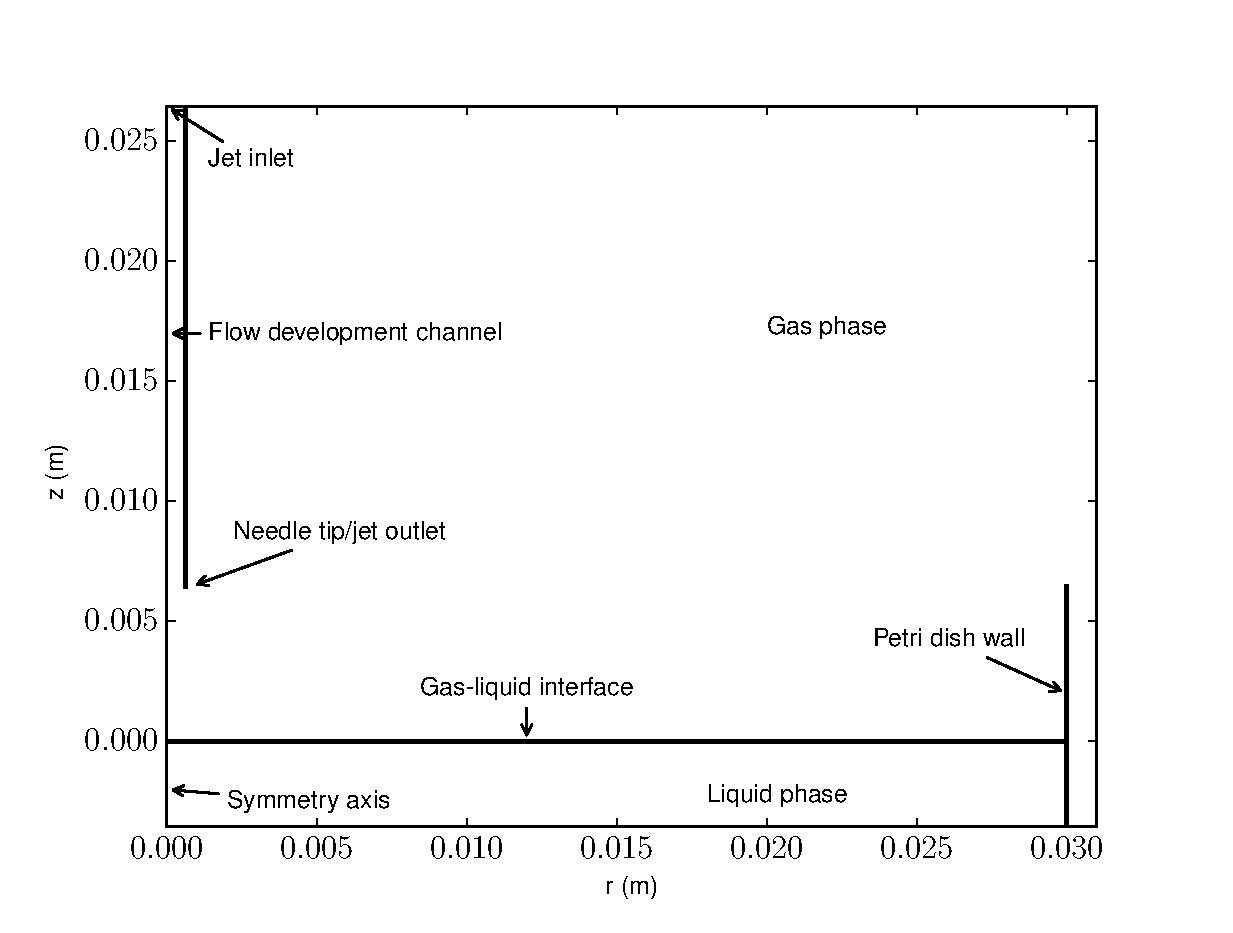
\includegraphics[width=\textwidth]{Geometry.eps}
        %\includegraphics[width=\textwidth]{Active_geometry_region.png}
    \caption{Experimental set-up for pulsed streamer-liquid system. Axis units are meters. The Python script used to create this figure, as well as the scripts used to create all subsequent figures can be found at \cite{scriptsLocation}}
    \label{fig:model_geom}
\end{figure}

\begin{table}[htpb]
    \begin{center}
        \begin{tabular}{|l| p{10cm}|}
            \hline
            Gas phase species & OH, H$_2$O$_2$, NO, NO$_2$, N$_2$O$_4$, HNO$_2$, HNO$_3$, H$_2$O \\
            \hline
            Liquid phase species & OH, H$_2$O$_2$, NO, NO$_2$, N$_2$O$_4$, HNO$_2$, NO$_2^-$, NO$_3^-$, ONOOH, H$^+$, OH$^-$ \\
            \hline
        \end{tabular}
    \end{center}
    \caption{Species included in the model}
    \label{tab:species_list}
\end{table}


\begin{table}[htpb]
    \begin{center}
        \begin{tabular}{|c |c |}
        \hline
        Needle diamater & 1.2 mm \\
        \hline
        Petri dish diameter & 6 cm \\
        \hline
        Gap distance & 6.5 mm \\
        \hline
        Water volume & 10 mL \\
        \hline
        Jet channel length & 2 cm \\
        \hline
        Maximum axial velocity of ionic wind/jet & 7.75 m/s \\
        \hline
        \end{tabular}
    \end{center}
    \caption{General model inputs}
    \label{tab:gen_inputs}
\end{table}

%\begin{minipage}[t]{0.25\textwidth}
    \begin{table}[htpb] %[H]
        \begin{center}
            \begin{tabular}{c |c }\rmfamily
                Molecule & H$_i$ [unitless] \\ \hline \hline
                OH & $6.92\cdot10^2$\\
                H$_2$O$_2$ & $1.92\cdot10^6$\\
                NO & $4.4\cdot10^{-2}$\\
                NO$_2$ & $2.8\cdot10^{-1}$\\
                N$_2$O$_4$ & $3.69\cdot10^1$\\
                HNO$_2$ & $1.15\cdot10^3$\\
                HNO$_3$ & $4.8\cdot10^6$\\
                HOONO & $4.8\cdot10^6$\\
            \end{tabular}
    \end{center}
        \caption{The Henry's constant for a number of molecules\cite{Tian2014}.}
        \label{tab:henryconstants}
    \end{table}
%\end{minipage}

%\begin{minipage}[t]{0.1\textwidth}
 %   \hspace{1cm}
%\end{minipage}

%\begin{minipage}[t]{0.25\textwidth}
    \begin{table}[htpb] %[H]
        \begin{center}
            \begin{tabular}{c |c |c}\rmfamily
                Molecule & D [m$^2$ s$^{-1}$]& reference\\ \hline \hline
                OH(g) & $4\cdot10^{-5}$ & \cite{Sakiyama2012b}\\
                H$_2$O$_2$(g) & $2\cdot10^{-5}$ & \cite{Sakiyama2012b}\\
                NO(g) & $2\cdot10^{-5}$ & \cite{Sakiyama2012b}\\
                NO$_2$(g) & $1.7\cdot10^{-5}$ & \cite{Sakiyama2012b}\\
                N$_2$O$_4$(g) & $1\cdot10^{-5}$ & \cite{Sakiyama2012b}\\
                HNO$_2$(g) & $2.1\cdot10^{-5}$ & \cite{Sakiyama2012b}\\
                HNO$_3$(g) & $2.1\cdot10^{-5}$ & \cite{Sakiyama2012b}\\
                H$_2$O(g) & $2.3\cdot10^{-5}$ & \cite{Sakiyama2012b}\\
                OH(aq) & $2.8\cdot10^{-9} [310 K]$ & \cite{khalack2005solvation}\\
                H$_2$O$_2$(aq) & $1.7\cdot10^{-9}$ & \cite{mcmurtrie1948measurement}\\
                NO(aq) & $2.2\cdot10^{-9}$ & \cite{zacharia2005diffusivity}\\
                NO$_2$(aq) & $1.85\cdot10^{-9} [296 K]$ & \cite{skinn2013nitrogen}\\
                N$_2$O$_4$(aq) & $1.5\cdot10^{-9}$ & Estimate\\
                HNO$_2$(aq) & $2.5\cdot10^{-9}$ & By analogy with nitric acid\\
                HNO$_3$(aq) & $2.5\cdot10^{-9}$ & \cite{wills1971diffusion}\\
                ONOOH(aq) & $2.5\cdot10^{-9}$ & By analogy with nitric acid\\
                NO$^{-}_2$(aq) & $1.7\cdot10^{-9}$ & \cite{kreft2001individual}\\
                NO$^{-}_3$(aq) & $1.7\cdot10^{-9}$ & \cite{kreft2001individual}\\
                H$^{+}$(aq) & $7\cdot10^{-9}$ & \cite{agmon1995grotthuss}\\
                OH$^{-}$(aq) & $5.29\cdot10^{-9}$ & \cite{kitamura1994microchemistry}\\
            \end{tabular}
        \end{center}
        \caption{The diffusion coefficients for a number of molecules at 300 K. See text for implementation of temperature dependence.}
        \label{tab:diffusioncoef}
    \end{table}
%\end{minipage}

\begin{table}[htpb]
    \begin{center}
        \begin{tabular}{c |c}\rmfamily
           Molecule & Molecule inlet concentration [m$^{-3}$]\\ \hline \hline
            OH & $1.3\cdot10^{18}$ \\
            H$_2$O$_2$ & $1.6\cdot10^{17}$ \\
            NO & $8\cdot10^{18}$ \\
            NO$_2$ & $5\cdot10^{16}$ \\
            N$_2$O$_4$ & 0 \\
            HNO$_2$ & $8\cdot10^{17}$ \\
            HNO$_3$ & $9\cdot10^{16}$ \\
            H$_2$O & 0 \\
        \end{tabular}
    \end{center}
    \caption{Gaseous species inlet concentrations. \cite{Tian2014} See text for discussion}
    \label{tab:inletconc}
\end{table}

\setcounter{magicrownumbers}{21}

\begin{ThreePartTable}
      \begin{TableNotes}
      \end{TableNotes}
      \begin{longtable}{>{\raggedright}m{3in} >{\raggedright}m{2in} >{\raggedright\arraybackslash}m{1.25in}}
            \textbf{Reaction} & \textbf{Rate coefficient} (Units of s$^{-1}$, m$^3$ mol$^{-1}$ s$^{-1}$, or m$^6$ mol$^{-2}$ s$^{-1}$. Temperature in K. Concentration of M in gas and H$_2$O in liquid are lumped into rate coefficient) & \textbf{Reference} \\ \hline \hline
            \endhead
            \caption{Reactions considered in model}
            \endfoot
            \caption{Reactions considered in model}
            \label{tab:rxns}
            \endlastfoot

            Gas phase reactions & & \\\hline
            1. 2NO$_2 \rightarrow$ N$_2$O$_4$ & $6.02\cdot10^5\cdot(300/T)^{3.8}$ & \cite{Sakiyama2012b} \\\hline
            2. N$_2$O$_4 \rightarrow$ 2NO$_2$ & $4.4\cdot10^6\cdot exp(-4952/T)$ & \cite{Sakiyama2012b} \\\hline
            3. NO + OH + M $\rightarrow$ HNO$_2$ + M & $1.1\cdot10^{7}\cdot(300/T)^{2.4}$ & \cite{Sakiyama2012b} \\\hline
            4. NO + NO$_2$ + H$_2$O $\rightarrow$ 2HNO$_2$ & 22 & \cite{wayne1951kinetics} \\\hline
            5. 2OH + M $\rightarrow$ H$_2$O$_2$ + M & $1.0\cdot10^7\cdot(T/300)^{-0.8}$ & \cite{Sakiyama2012b} \\\hline
            6. NO$_2$ + OH + M $\rightarrow$ HNO$_3$ + M & $3.2\cdot10^7\cdot(300/T)^{2.9}$ & \cite{Sakiyama2012b} \\\hline
            7. OH + HNO$_2$ $\rightarrow$ NO$_2$ + H$_2$O & $3.0\cdot10^6\cdot exp(-390/T)$ & \cite{Sakiyama2012b} \\\hline
            8. 2HNO$_2$ $\rightarrow$ NO + NO$_2$ + H$_2$O & $6.0\cdot10^{-3}$ & \cite{Sakiyama2012b} \\\hline
            9. HNO$_2$ + HNO$_3$ $\rightarrow$ 2NO$_2$ + H$_2$O & 9.6 & \cite{Sakiyama2012b} \\\hline
            10. HNO$_3$ + NO $\rightarrow$ HNO$_2$ + NO$_2$ & $4.4\cdot10^{-3}$ & \cite{dorai2002modeling} \\\hline
            \\
            Liquid phase reactions & & \\\hline
            11. N$_2$O$_4$ + H$_2$O $\rightarrow$ NO$_2^-$ + NO$_3^-$ + 2H$^+$ & 1000 & \cite{coddington1999hydroxyl} \\\hline
            12. 2NO$_2$ + H$_2$O $\rightarrow$ NO$_2^-$ + NO$_3^-$ + 2H$^+$ & $8.4\cdot10^{4}\cdot exp(-0.033\cdot(T-295))$ & \cite{park1988solubility} \\\hline
            13. NO + NO$_2$ + H$_2$O $\rightarrow$ 2NO$_2^-$ + 2H$^+$ & $1.6\cdot10^{5}$ & \cite{park1988solubility} \\\hline
            \ONOOHlong{}. NO$_2^-$ + H$_2$O$_2$ + H$^+$ $\rightarrow$ ONOOH + H$_2$O & $1.1\cdot10^{-3}$ & \cite{Lukes2014b}\\\hline
            \OHfromONOOH{}. ONOOH $\rightarrow$ .7(NO$_3^-$ + H$^+$) + .3(NO$_2$ + OH) & .8 & \cite{coddington1999hydroxyl}\\\hline
            \ONOOHshort{}. NO$_2$ + OH $\rightarrow$ ONOOH & $5.3\cdot10^{6}$ & \cite{Lukes2014b,goldstein2005chemistry}\\\hline
            17. 2OH + M $\rightarrow$ H$_2$O$_2$ + M & $1\cdot10^{7}\cdot exp(-450\cdot(1/T-1/298))$ & \cite{johnaelliot1990estimation}\\\hline
            18. HNO$_2$ $\rightarrow$ H$^+$ + NO$_2^-$ & $3.51\cdot10^{6}$ & From reaction \NitrousAcidAssociation{} and equilibrium constant \\\hline
            \NitrousAcidAssociation{}. H$^+$ + NO$_2^-$ $\rightarrow$ HNO$_2$ & $7\cdot10^{6}$ & Assumes diffusion limited\\\hline
            \WaterAssociation{}. H$^+$ + OH$^-$ $\rightarrow$ H$_2$O & $7\cdot10^{6}$ & Assumes diffusion limited \\\hline
            21. H$_2$O $\rightarrow$ H$^+$ + OH$^-$ & $7\cdot10^{-2}$ & From reaction \WaterAssociation{} and equilibrium constant\\\hline
            22. NO + OH $\rightarrow$ HNO$_2$ & $2\cdot10^{7}$ & \cite{Tian2014}\\\hline
	    23. 2HNO$_2$ $\rightarrow$ NO + NO$_2$ & $1.34\cdot10^{-2}\cdot exp(.106\cdot(T-295))$ & \cite{park1988solubility}\\\hline
            \\
            Tyrosine reactions & & \\\hline
            \rownumber. NO$_2$ + Tyr $\rightarrow$ NO$_2^-$ + Tyr(radical) & $2.90\cdot10^4$ & \cite{goldstein2000tyrosine}\\\hline
            \rownumber. Tyr(radical) + NO $\rightarrow$ Tyr-NO & $1.00\cdot10^6$ & \cite{goldstein2000tyrosine}\\\hline
            \rownumber. Tyr-NO $\rightarrow$ Products & 2 & \cite{goldstein2000tyrosine}\\\hline
            \rownumber. Tyr-NO $\rightarrow$ Tyr(radical) + NO & $1\cdot10^3$ & \cite{goldstein2000tyrosine}\\\hline
            \rownumber. Tyr(radical) + Tyr(radical) $\rightarrow$ diTyr & $2.25\cdot10^5$ & \cite{goldstein2000tyrosine}\\\hline
            \rownumber. NO$_2$ + Tyr(radical) $\rightarrow$ Tyr-NO$_2$ & $1.30\cdot10^6$ & \cite{goldstein2000tyrosine}\\\hline
            \rownumber. NO$_2$ + Tyr(radical) $\rightarrow$ Other products & $1.70\cdot10^6$ & \cite{goldstein2000tyrosine}\\\hline
            \rownumber. Tyr + OH $\rightarrow$ TyrOHo & $7\cdot10^6$ & \cite{solar1984reactivity}\\\hline
            \rownumber. Tyr + OH $\rightarrow$ TyrOHm & $5\cdot10^6$ & \cite{solar1984reactivity}\\\hline
            \rownumber. Tyr + OH $\rightarrow$ Tyr(radical) & $6\cdot10^5$ & \cite{solar1984reactivity}\\\hline
            \rownumber. TyrOHm + TyrOHm $\rightarrow$ products & $1\cdot10^6$ & \cite{solar1984reactivity}\\\hline
            \rownumber. TyrOHo + TyrOHo $\rightarrow$ products & $1.5\cdot10^5$ & \cite{solar1984reactivity}\\\hline
            \rownumber. TyrOHo $\rightarrow$ Tyr(radical) + H$_2$O & $1.8\cdot10^4$ & \cite{solar1984reactivity}\\\hline
        \end{longtable}
\end{ThreePartTable}

\subsection{Results and Discussion}

The steady state velocity field is shown in figure \ref{fig:v_field}. The recirculating pattern observed in the gas phase is consistent with the corona discharge modelling results reported in \cite{Zhao2005a}. A similar recirculation pattern is observed in the liquid phase, induced by shear stresses between the phases at the gas-liquid interface. The maximum liquid phase velocity, .1 m/s, occurs along the interface approximately .8 mm away from the stagnation point (r = 0).

\begin{figure}[htb]
    \centering
        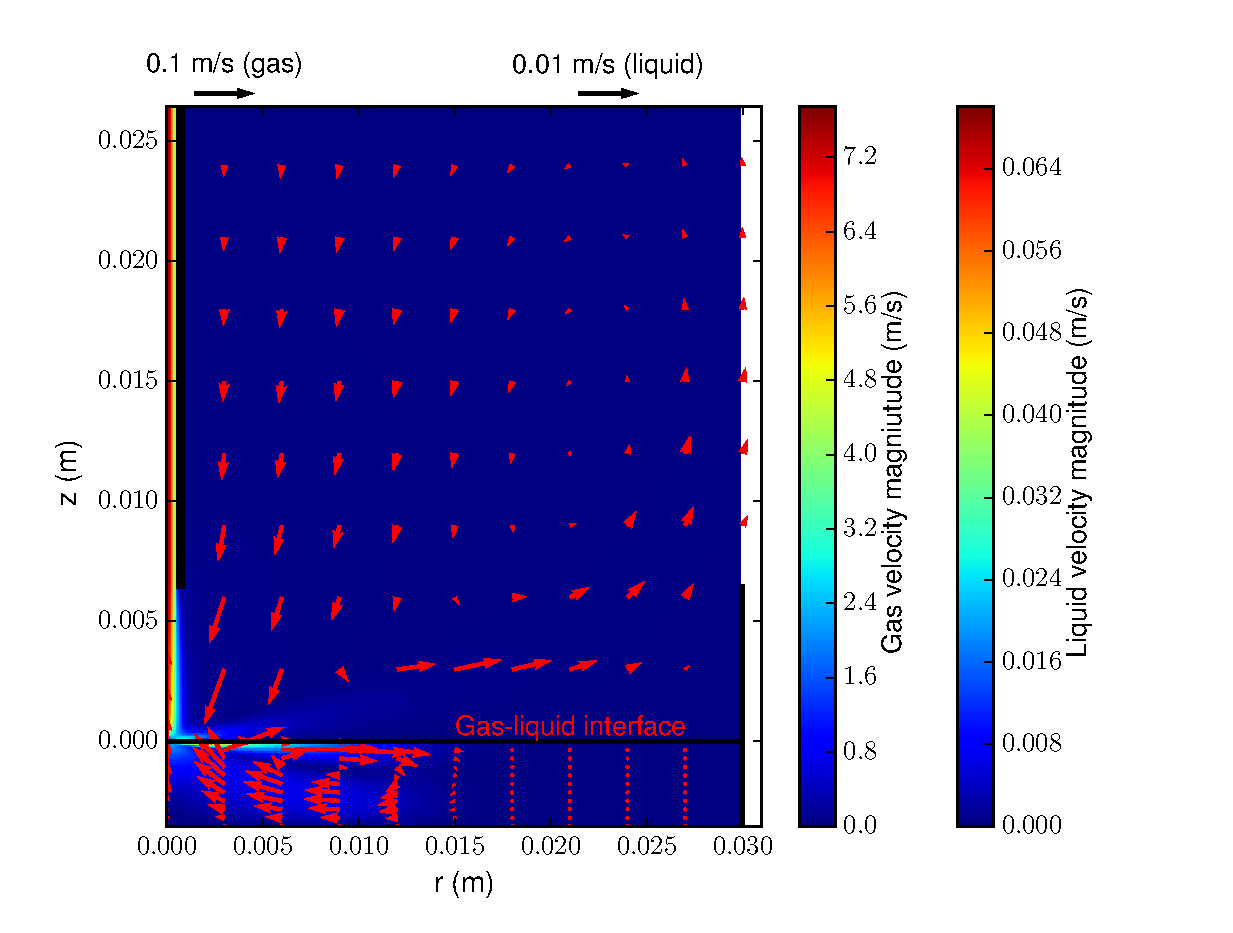
\includegraphics[width=\textwidth]{velocity.eps}
        %\includegraphics[width=\textwidth]{Fluid_flow.jpg}
    \caption{Velocity magnitude and direction. Axis units are meters. Interface is at z = 0. Axis of symmetry is at r = 0. Selected velocity vectors are overlaid on color scale indicating velocity magnitude. Red color represents higher values and blue color represents lower values. Velocity vector arrows are scaled 12.5 times larger in the aqueous phase.}
    \label{fig:v_field}
\end{figure}

The temperature and water vapor profiles at the end of the simulation (t = 1000 seconds) are shown in figures \ref{fig:temp_2D_profile} and \ref{fig:water_2D_profile}. Notably, the temperature in the bulk liquid has fallen close to 10 K from its initial value of 300 K. This drop in temperature in the bulk liquid is an example of the classical wet-bulb/dry-bulb problem found in chemical engineering texts. Water vapor present in the gas above the interface is whisked away by convection. In order to maintain the equilibrium vapor pressure required by Antoine's equation, liquid water must be evaporated, consuming heat and lowering the temperature at the interface. Heat then migrates from the bulk liquid to the surface, leading to bulk liquid cooling. In this problem we have assumed that the impinging gas is at room temperature, and subsequently convection-induced evaporation leads to cooling of the bulk liquid below room ambient. However, if there is significant plasma heating of the gas, it is possible that heating of the liquid above the initial temperature will be observed experimentally. The important point is that the natural coupling between heat transport and evaporation leads to significant spatial variation in temperature, particularly at the interface, and a cooling of the bulk liquid relative to the gas. An example of the steep temperature gradients is shown in figure \ref{fig:temp_1D_profile} where the gas phase temperature changes by 10 K over the span of 200 $\mu$m, immediately above the liquid surface. Because reaction rates typically exhibit Arrhenius dependence on temperature, physical factors that introduce steep temperature gradients should be included in any model that wishes to accurately predict plasma-liquid chemistry. Though not shown here, a simulation was conducted in which temperature and water-vapor transport were de-coupled and the interfacial temperature gradient removed. Compared to the coupled case, concentrations of long-lived aqueous species like H$_2$O$_2$, NO$_2^-$, and NO$_3^-$ differed by as large as factors of two at the end of the simulation, demonstrating the importance of accounting for evaporation-induced temperature gradients.

Another instance of transport coupling that may impact plasma-liquid chemistry is the significant radial gradients in the concentration of water vapor between the needle tip/jet outlet and gas-liquid interface. An example of these gradients induced by convective forces are shown in figure \ref{fig:water_1D_profile}. Examining the dotted curve, which gives the radial distribution of water vapor half-way between the jet outlet/needle tip and liquid surface, one can see that the water vapor concentration drops precipitously in the region of the discharge (r $<$ 2 mm). In the center of the discharge (r $=$ 0) the water vapor concentration is essentially zero. This large drop in the concentration of water vapor in the active discharge region due to convection suggests that the concentrations of plasma species which rely on H$_2$O as a precursor will be reduced at increasing distances from the liquid surface, relative to  discharges where diffusion is the dominant mechanism of mass transport.

\begin{figure}[htb]
    \centering
        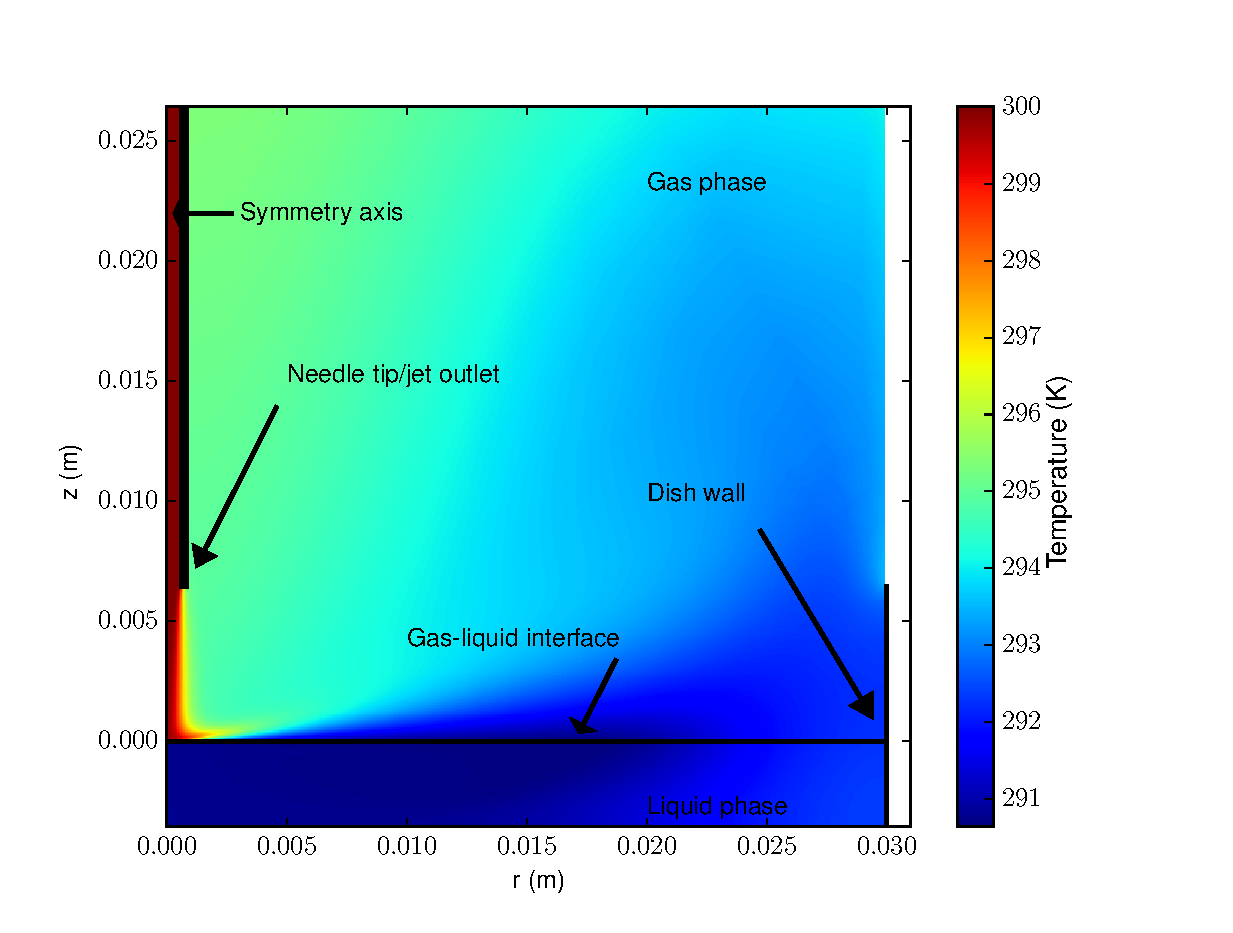
\includegraphics[width=\textwidth]{Temperature2D.eps}
        %\includegraphics[width=\textwidth]{Temperature.jpg}
        \caption{2D temperature profile at t = 1000 seconds. Red color represents higher values; blue color lower values. Inlet temperature is 300 K. Temperature in the bulk liquid has cooled by approximately 10 K because of convection-induced evaporative cooling.}
        \label{fig:temp_2D_profile}
\end{figure}

\begin{figure}[htb]
    \centering
        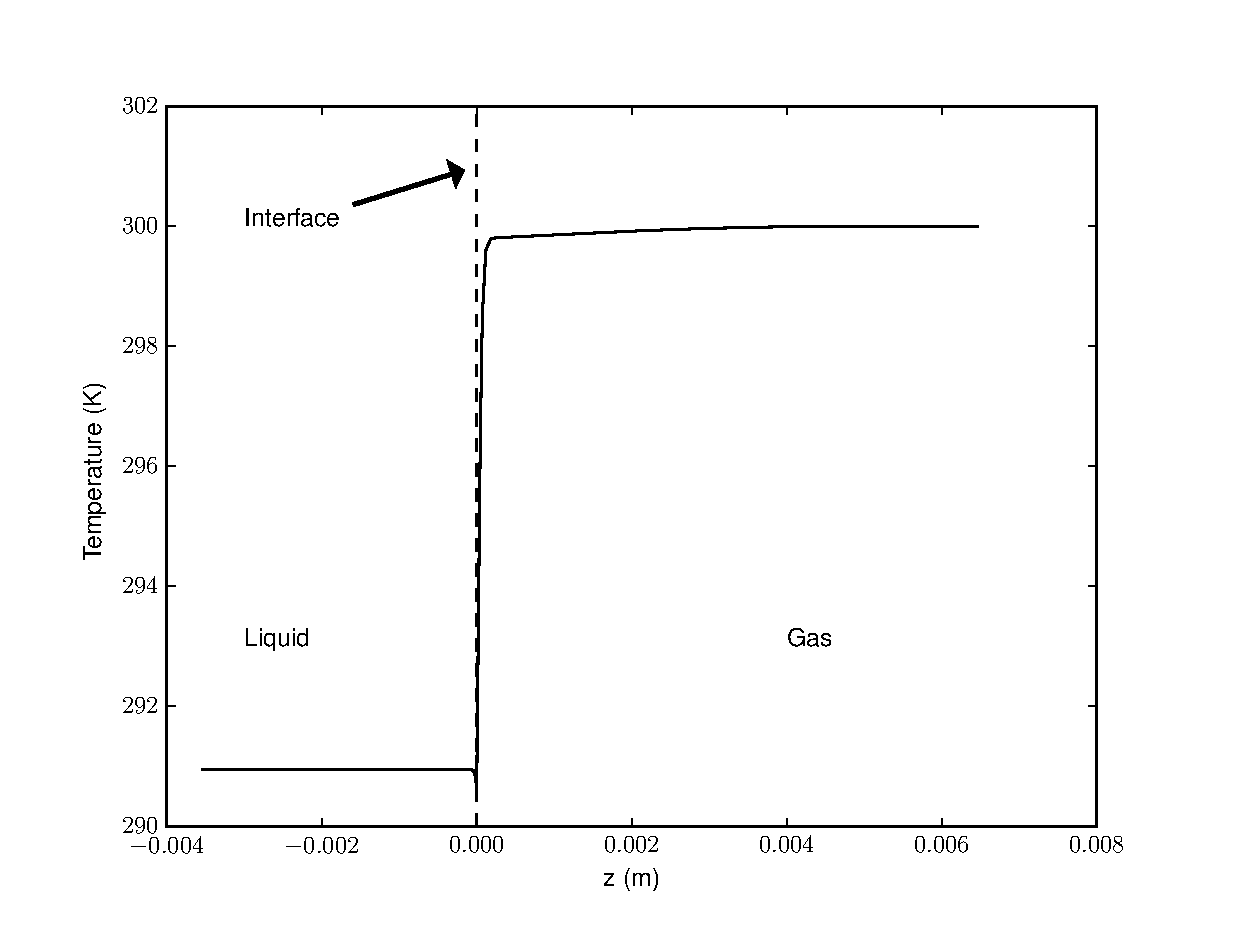
\includegraphics[width=\textwidth]{1D_temperature_plot.eps}
        \caption{Temperature along z-axis. Illustrates the large temperature gradient that exists at the gas-liquid interface and the resulting difference in bulk gas and liquid temperatures.}
        \label{fig:temp_1D_profile}
\end{figure}

\begin{figure}[htb]
    \centering
        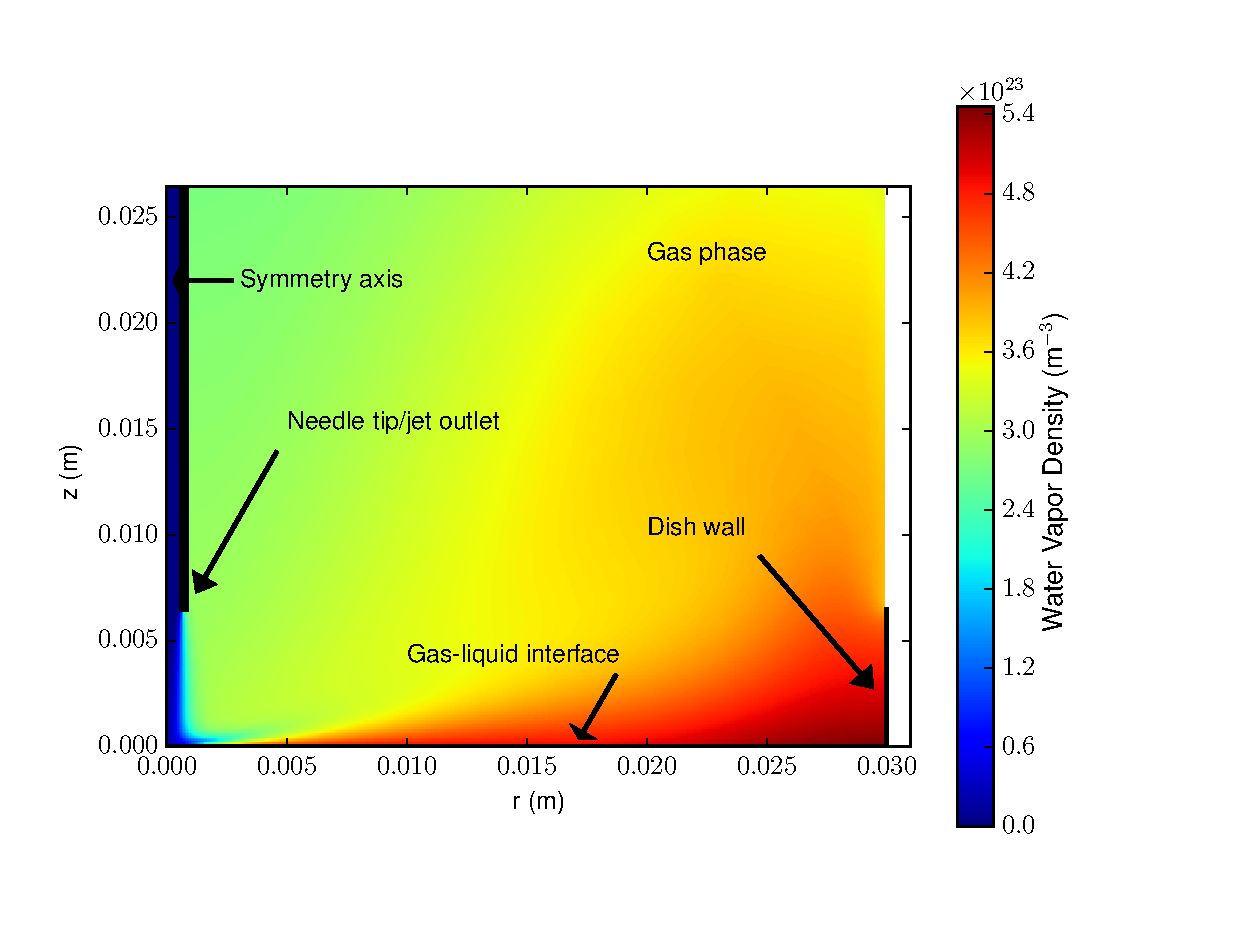
\includegraphics[width=\textwidth]{WaterVapor2D.eps}
        %\includegraphics[width=\textwidth]{Water_vapor.jpg}
        \caption{2-D water vapor profile at t = 1000 seconds. Red color represents higher values of water vapor concentration; blue color lower values. As implemented through Antoine's equation, water vapor concentration at the interface is highest where the temperature is highest. Role of convection in water vapor profile is evident in decreased concentration near the streamer/jet.}
        \label{fig:water_2D_profile}
\end{figure}


\begin{figure}[htb]
    \centering
        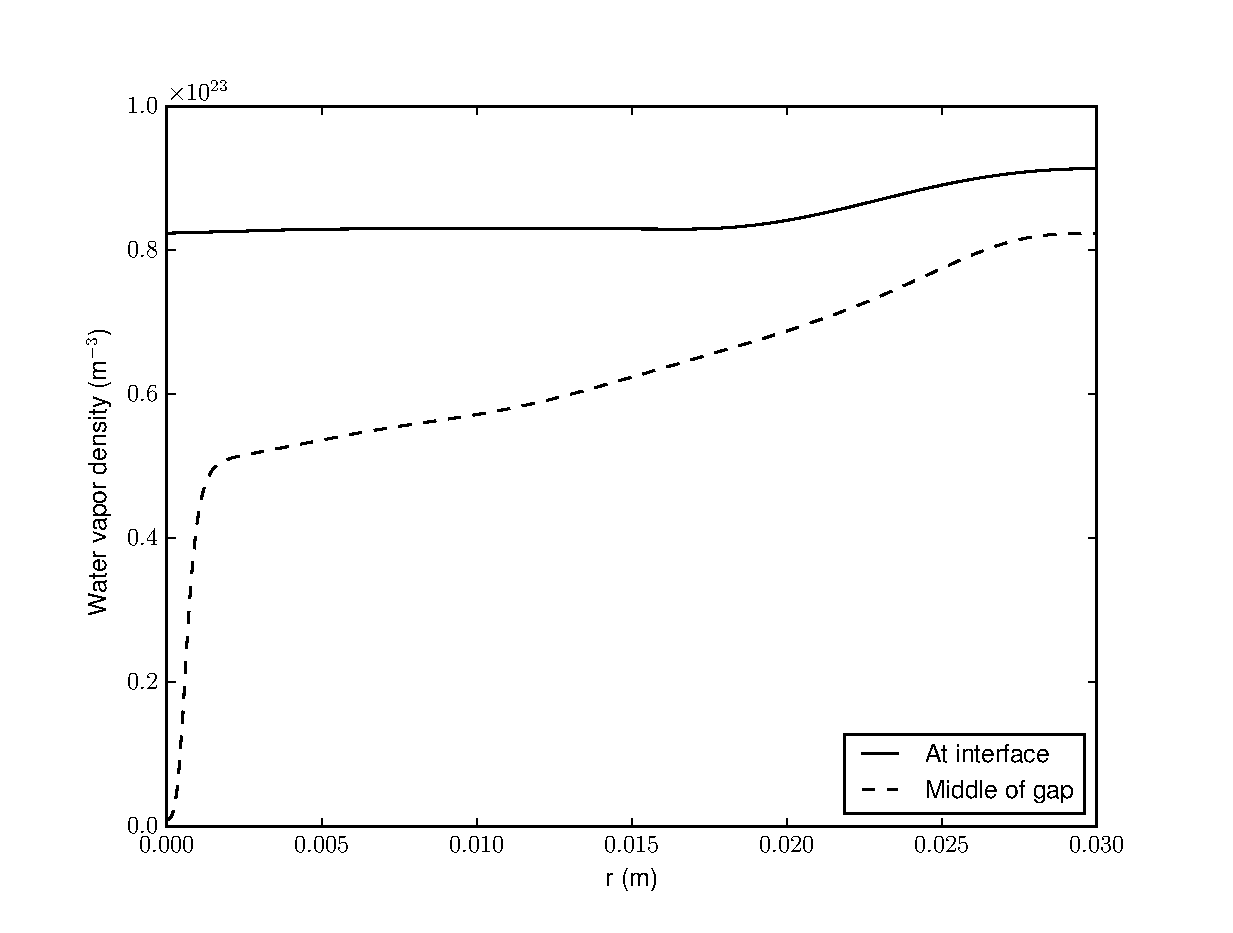
\includegraphics[width=\textwidth]{1D_water_vapor_plot.eps}
        \caption{Radial water vapor profiles. Horizontal axis is the radial coordinate. The top curve (solid) corresponds to the water vapor concentration at the interface. The bottom curve (dashed) shows the strong water vapor radial dependence in the middle of the streamer/jet gap. Gradient is largest near and inside the discharge region.}
        \label{fig:water_1D_profile}
\end{figure}

This model also addresses the role that convection plays in dissolution rates of different gaseous species. For this analysis, reactions are turned off, reducing mass transport to only convection and diffusion. As one might intuitively expect, the induced convective flow in the liquid significantly changes the spatial distribution of aqueous species relative to a diffusion only case, as demonstrated for HNO$_3$ in figures \ref{fig:HNO3_convec} and \ref{fig:HNO3_diffus} (note that gas convection is present in both figures). However, what is perhaps not intuitive is that though the HNO$_3$ spatial distribution changes dramatically depending on whether convection is present in the liquid, the volume-averaged uptake of HNO$_3$ does not change from diffusion-dominated to convection-dominated cases as shown in figure \ref{fig:HNO3_mass_compare}. If a hydrophobic specie like NO is examined instead of a hydrophilic specie like HNO$_3$, it is observed that the presence of liquid convection increases volume-averaged uptake significantly, as illustrated in figure \ref{fig:NO_mass_compare}. This fundamental difference in behavior between hydrophilic and hydrophobic species can be explained in terms of lumped mass transfer resistances. For a hydrophilic specie, the dominant resistance to interfacial transfer is in the gas-phase, whereas for a hydrophobic specie the dominant resistance to transfer occurs in the liquid phase. \cite[p. 249]{carberry2001chemical} Consequently, when convection is added to the liquid phase, effectively reducing the liquid-side mass transfer resistance, the overall resistance to mass transfer decreases and the volume-averaged uptake increases significantly for hydrophobic species like NO whereas the change in overall resistance is miniscule for hydrophilic species like HNO$_3$.

\begin{figure}[htpb]
    \centering
    \begin{subfigure}[b]{.7\textwidth}
        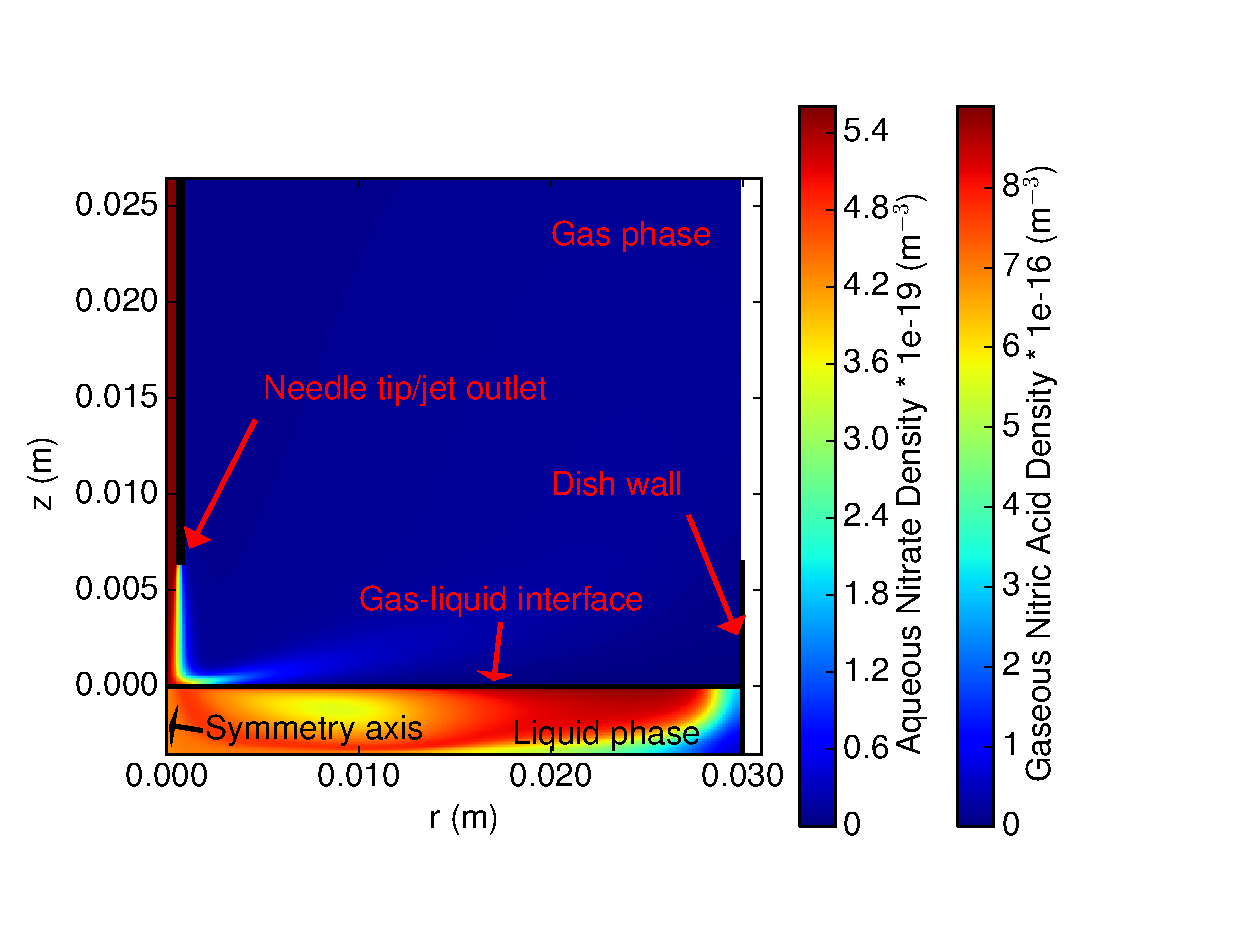
\includegraphics[width=\textwidth]{HNO3Convection2D.eps}
        \caption{Distribution of HNO$_3$ with liquid convection turned on. t = 1000 s}
        \label{fig:HNO3_convec}
    \end{subfigure}
    %\quad
    \begin{subfigure}[b]{.7\textwidth}
        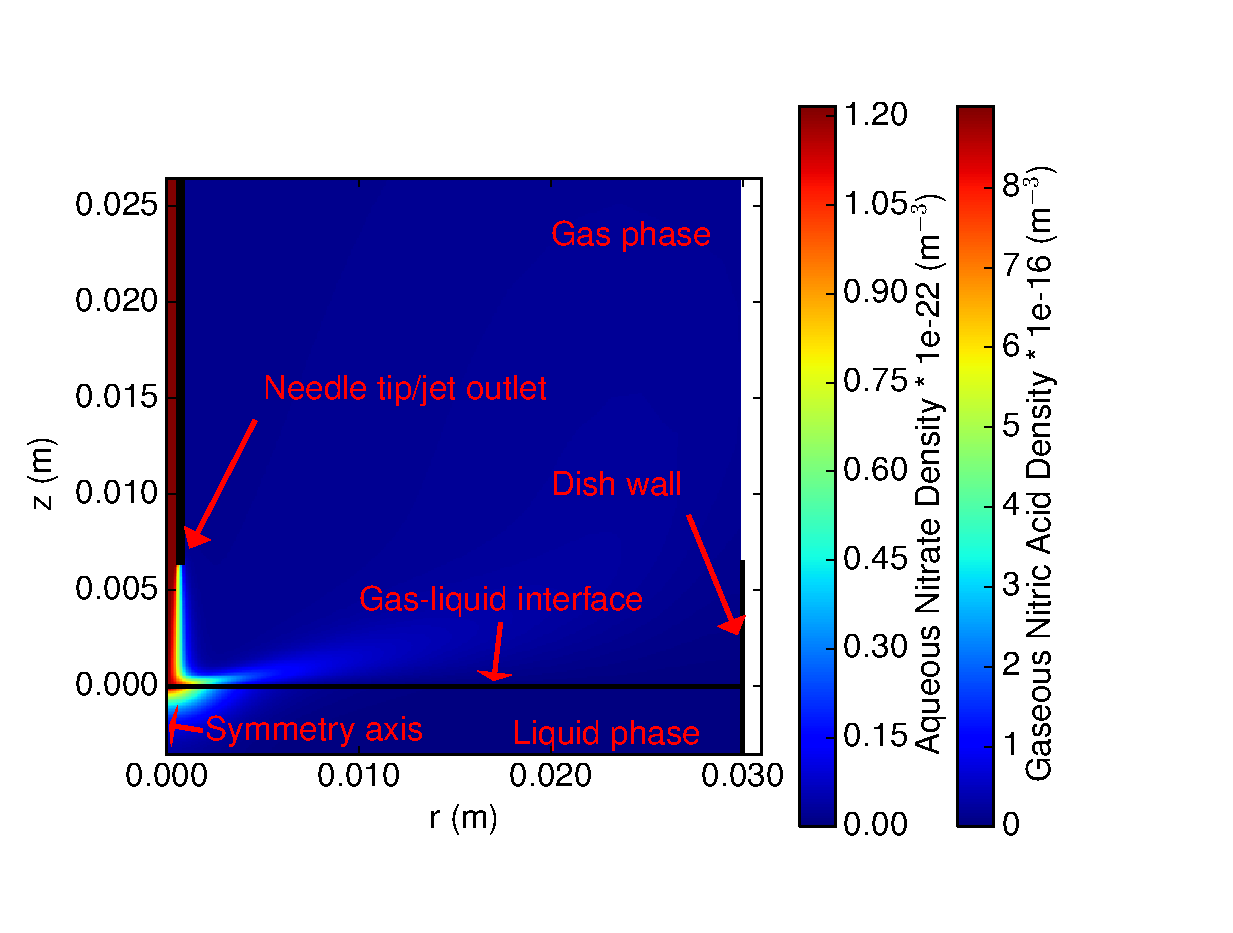
\includegraphics[width=\textwidth]{HNO3Diffusion2D.eps}
        \caption{Distribution of HNO$_3$ with liquid convection turned off. t = 1000 s}
        \label{fig:HNO3_diffus}
    \end{subfigure}
    \caption{}
    \label{fig:HNO3}
\end{figure}

\begin{figure}[htpb]
    \centering
    \begin{subfigure}[b]{.63\textwidth}
        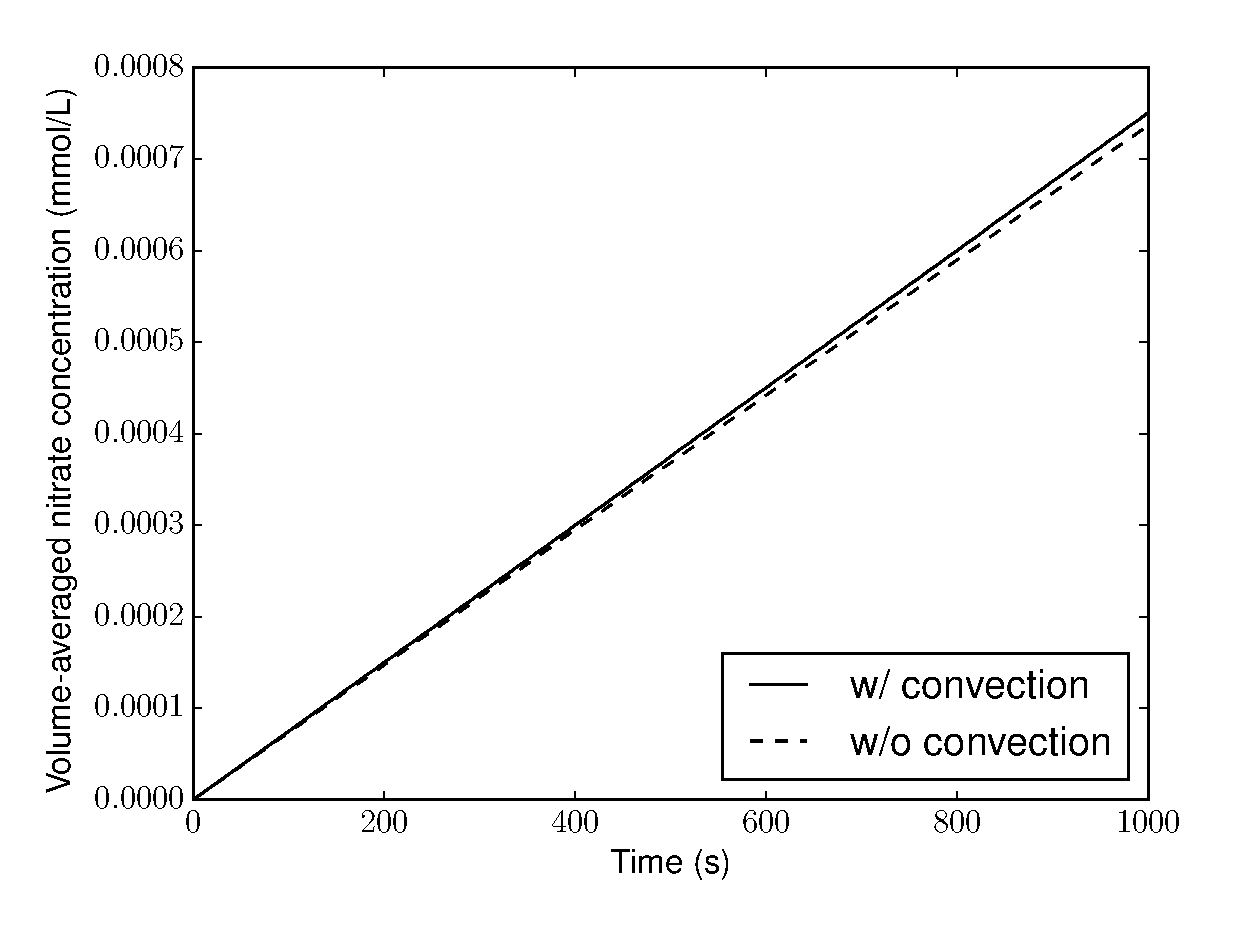
\includegraphics[width=\textwidth]{Nitrate_uptake_plot.eps}
        \caption{Comparison of volume averaged uptake of nitrate (HNO$_3$ before dissolution) with liquid convection toggled on or off. Very little difference between the two cases.}
        \label{fig:HNO3_mass_compare}
    \end{subfigure}
    %\quad
    \begin{subfigure}[b]{.63\textwidth}
        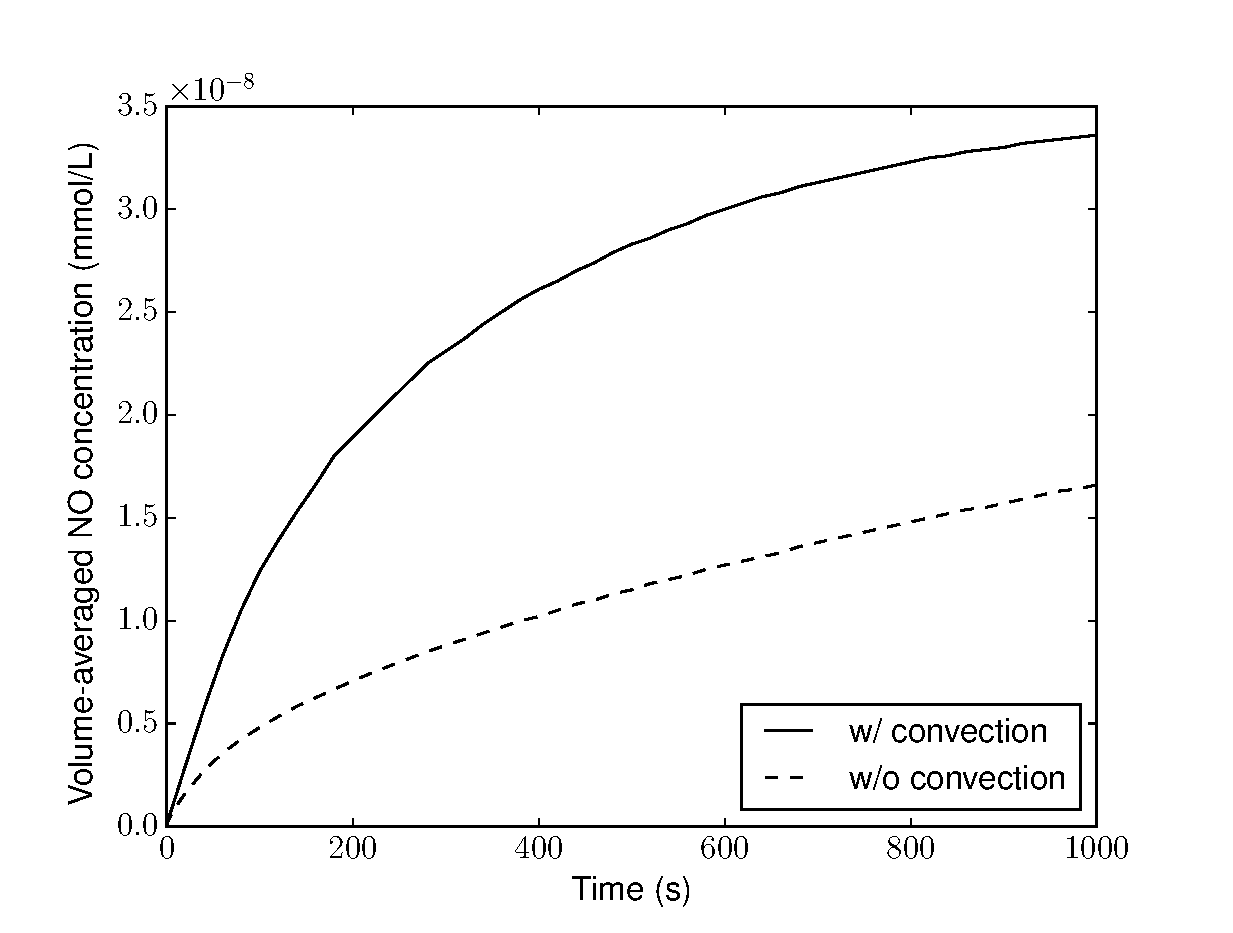
\includegraphics[width=\textwidth]{NO_uptake_plot.eps}
        \caption{Comparison of volume averaged uptake of NO with liquid convection toggled on or off. The presence of convection increases the volume-averaged concentration by roughly a factor of 2 over the course of the simulation. Note that the vertical scale is much smaller for NO than for HNO$_3$ in \ref{fig:HNO3_mass_compare} because of NO's hydrophobicity}
        \label{fig:NO_mass_compare}
    \end{subfigure}
    \caption{}
    \label{fig:excel}
\end{figure}

When the full reaction set is considered, large gradients in reactive species concentrations emerge at the interface. Of particular interest for biomedical or pollutant degradation applications is the distribution of hydroxyl radical in the aqueous phase. Figure \ref{fig:log_OH_conc} shows a 3D plot of the base 10 log of OH(aq) concentration versus radial and axial position for t = 1000 seconds. Interfacial gradients in OH concentration are prominent in the region where the discharge impinges on the water surface. At the stagnation point (r=0) the OH concentration drops by approximately 9 orders of magnitude over the span of 50 $\mu$m in the axial direction. Moving away from where the streamer/jet touches the surface, the interfacial gradients become less pronounced. Even so, the largest OH concentration away from the surface and in the bulk solution is 3-4 orders of magnitude lower than the peak OH concentration which occurs at the interface and at the center of the impinging streamer/jet. The presence of the liquid phase convective loop is evident from the OH concentration hole in the center of Figure \ref{fig:log_OH_conc}. The effect is also seen in the center of Figure \ref{fig:log_ONOOH_conc} for ONOOH.

\begin{figure}[htb]
    \centering
    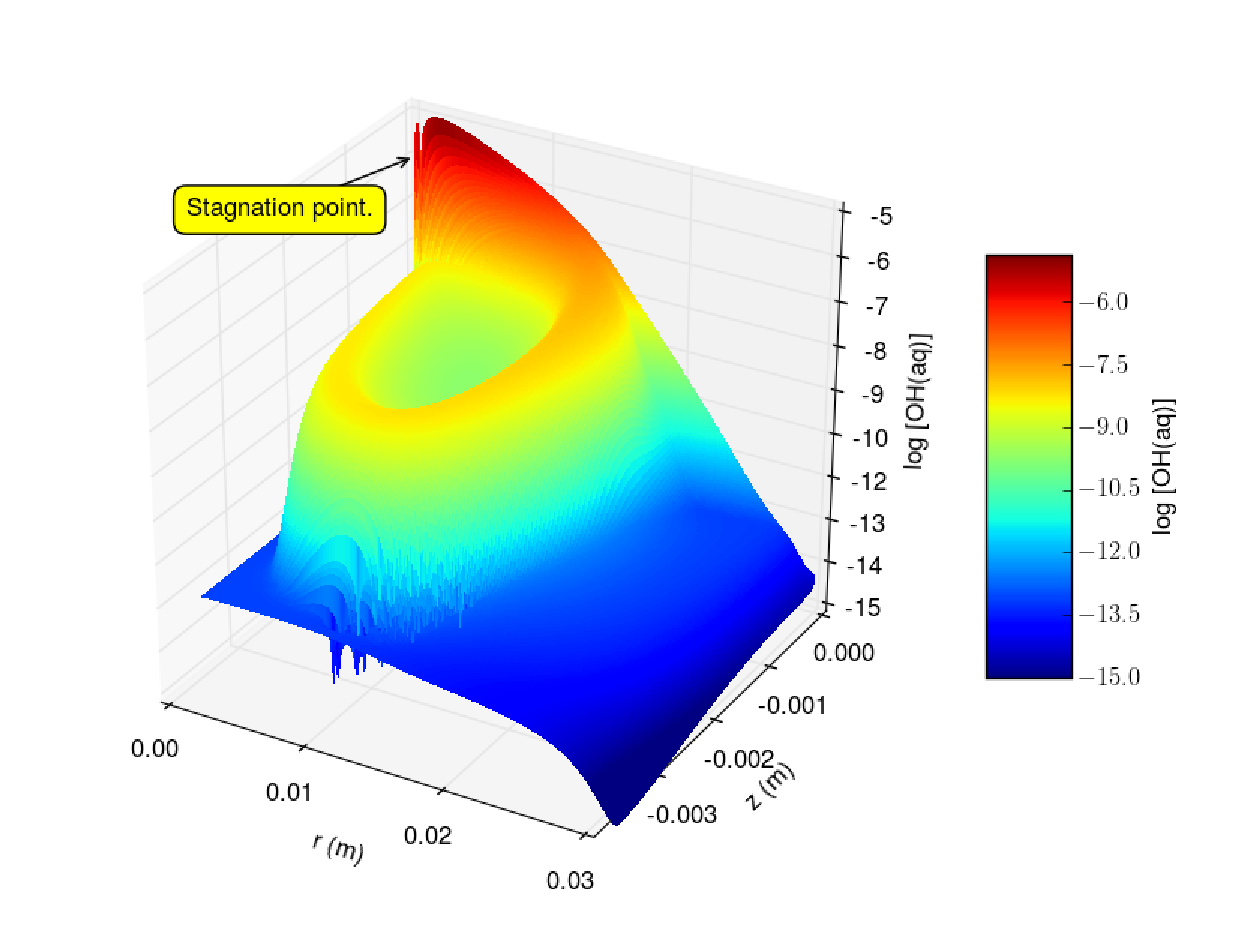
\includegraphics[width=\textwidth]{logOH.eps}
    \caption{3D plot of log$_{10}$(OH(aq)) as a function of position for t = 1000 seconds. Large interfacial gradients are evident, particularly at the stagnation point (r=z=0). Note the effect of convection in the hole in OH concentration in the center of the plot. Some numerical noise is observed at very low OH concentrations towards the bottom of the dish. Note that the r and z axes have different scales}
    \label{fig:log_OH_conc}
\end{figure}

Another plasma-generated specie which has received much attention in the literature is peroxynitrous acid and its conjugate base peroxynitrite. In the current model, ONOOH exists only in the liquid phase and can be created through two mechanisms: reactions \ONOOHlong{} and \ONOOHshort{} in table \ref{tab:rxns}. Reaction \ONOOHlong{} was the topic of an excellent study in \cite{Lukes2014b} and is hypothesized to be a key player in the long-term anti-bacterial efficacy of plasma activated water. Figure \ref{fig:log_ONOOH_conc} shows the base 10 log of ONOOH concentration as a function of r and z in the aqueous phase. As with OH, there are large interfacial concentration gradients. At r=0, the ONOOH concentration drops by 5 orders of magnitude over 30 $\mu$m in the axial direction. Away from the stagnation point, especially where the convective current flows away from the interface, the interfacial gradient is much smaller but again as with OH, the highest bulk concentration is orders of magnitude lower than the peak surface concentration. The reason for these large ONOOH gradients is the relative dominance of reaction \ONOOHshort{} over reaction \ONOOHlong{} for the given model inputs. Over the course of the simulation, almost 7000 times more ONOOH is produced through the reaction of OH and NO$_2$ than through the reaction of H$^+$, H$_2$O$_2$, and NO$_2^-$. As shown in figure \ref{fig:log_OH_conc}, hydroxyl does not penetrate any more than a few tens of microns into the liquid phase, so consequently all ONOOH produced through OH is produced within a few tens of microns of the liquid surface. If we examine the production of ONOOH through reaction \ONOOHlong{}, it is observed to be much more uniform as illustrated in figure \ref{fig:log_ONOOH_prod_rate}. This is because of the relative uniformity in concentration of H$^+$, NO$_2^-$, and H$_2$O$_2$, although there is a peak in their concentrations and consequently in their production of ONOOH in the vicinity of the impinging streamer/jet. Once the streamer is turned off and surface fluxes of ON and NO$_2$ are removed, production of ONOOH(aq) will proceed almost exclusively through reaction \ONOOHlong{}, resulting in a mostly homogeneous distribution. This is relevent for applications of PAW since ONOOH is the long-term intermediary for production of OH through reaction \OHfromONOOH{}.

\begin{figure}[htb]
    \centering
    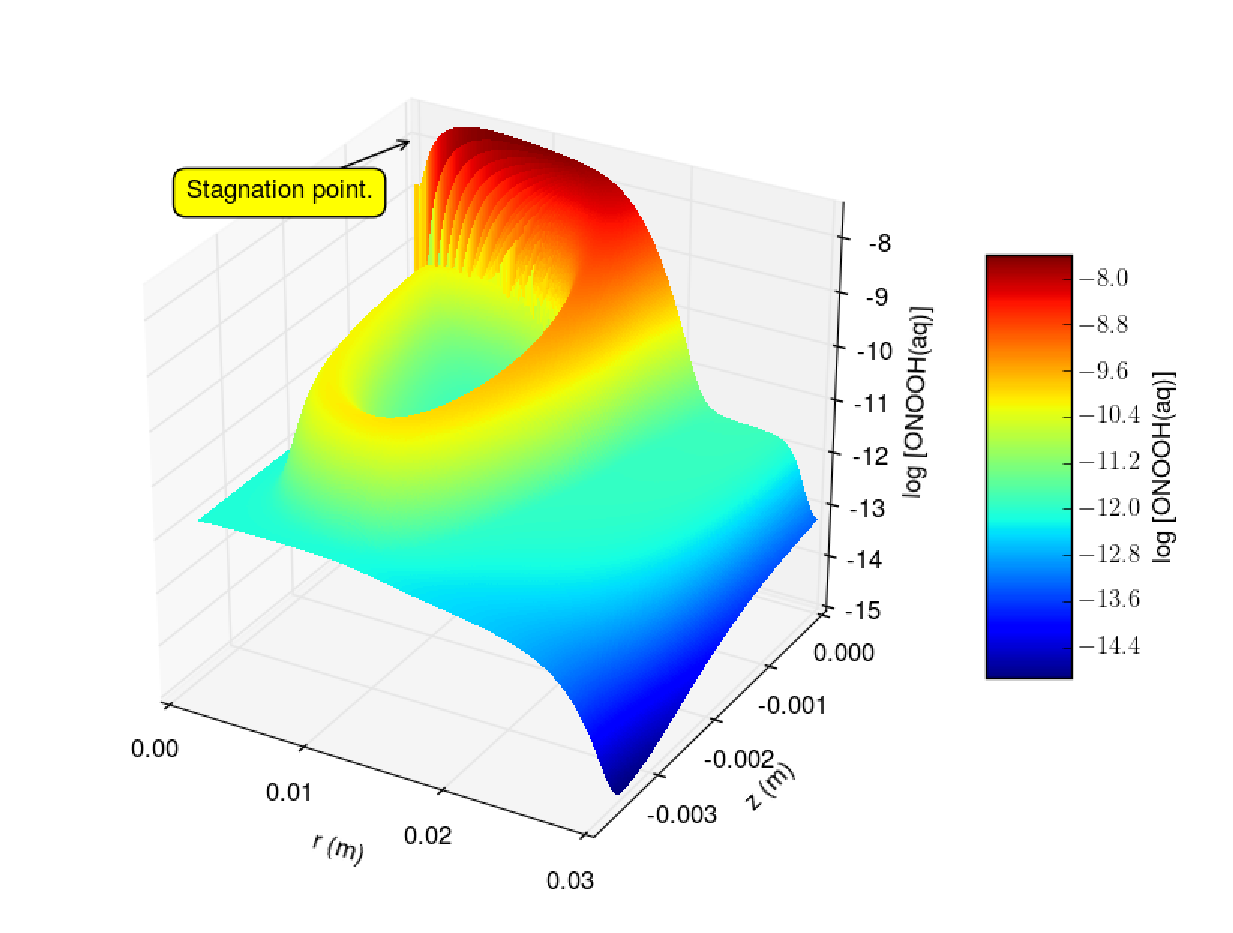
\includegraphics[width=\textwidth]{logONOOH.eps}
    \caption{3D plot of log$_{10}$(ONOOH(aq)) as a function of position for t = 1000 seconds. As with OH, large interfacial gradients are evident as is the effect of the liquid convection loop. Note that the r and z axes have different scales}
    \label{fig:log_ONOOH_conc}
\end{figure}

\begin{figure}[htb]
    \centering
    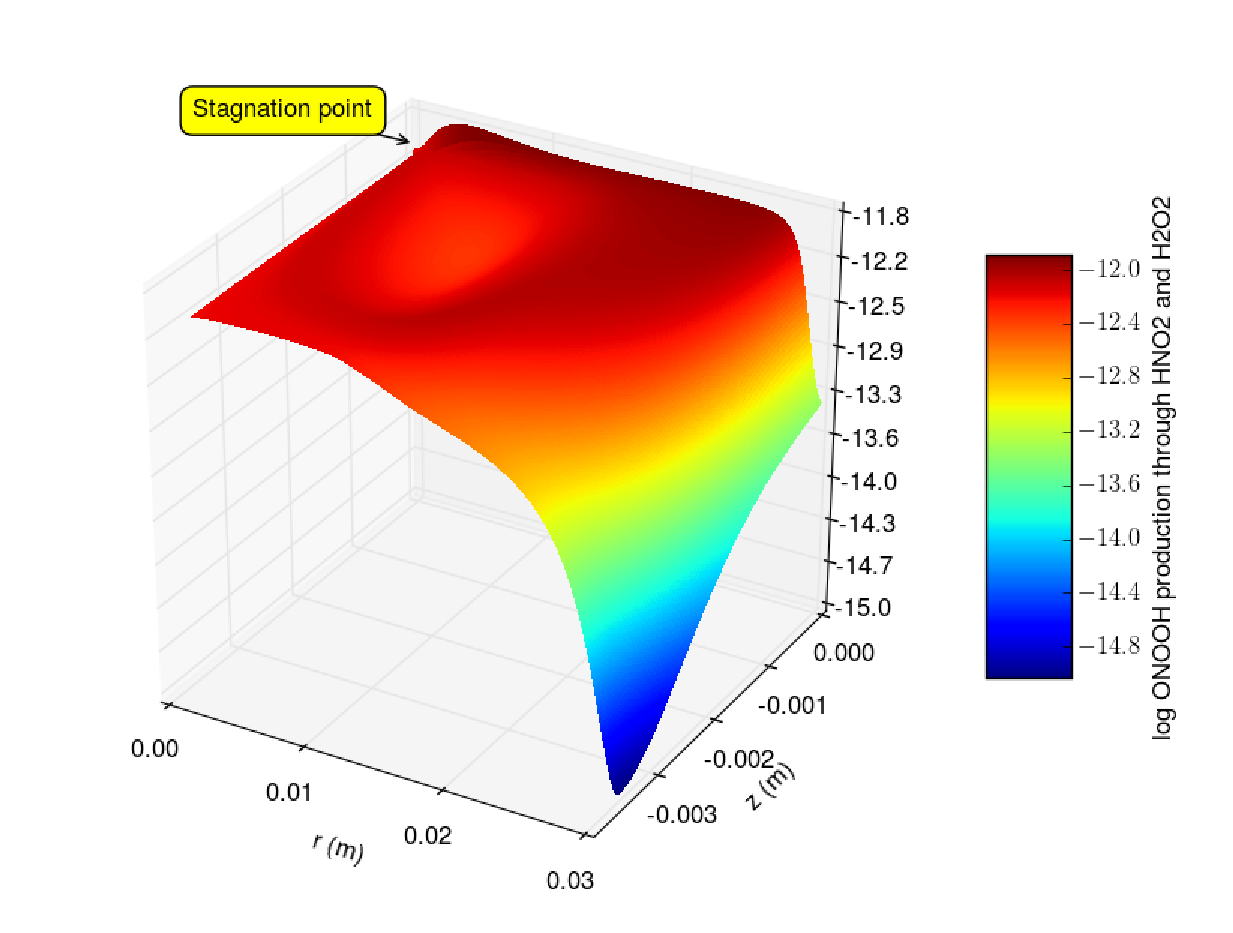
\includegraphics[width=\textwidth]{logONOOHproduced.eps}
    \caption{3D plot of the base 10 logarithm of the producation rate of ONOOH through reaction \ONOOHlong{} listed in table \ref{tab:rxns}. Because of the relative uniformity in the distribution of H$^+$, H$_2$O$_2$, and NO$_2^-$, the production of ONOOH through reaction \ONOOHlong{} is much more uniform than the overall concentration profile of ONOOH. Note that the r and z axes have different scales.}
    \label{fig:log_ONOOH_prod_rate}
\end{figure}

The results presented here suggest two different regimes of activity in the solution: surface and bulk. When the discharge is on, reactivity in the form of OH is confined almost entirely to the plasma-liquid interface. Bulk solution concentrations of OH are several orders of magnitude lower than the surface concentration. This is also true of other potentially biologically important and highly reactive reagents such as NO and NO$_2$ radicals. Less reactive plasma-generated RONS like H$_2$O$_2$ and NO$_2^-$ have significantly longer lifetimes and can be transported into the bulk solution where they can react and form ONOOH, a precursor to OH and NO$_2$. However, for the model inputs used here, the bulk reactivity generated through H$_2$O$_2$ and NO$_2^-$ precursors is orders of magnitude less on a per unit time scale than the surface reactivity coming from direct fluxes of plasma generated radicals. When the discharge is turned off, generation of reactive species through H$_2$O$_2$ and NO$_2^-$ will persist for a while in the bulk. The results in \cite{Lukes2014b} show a nitrite half-life of 2-3 hours in acidic solution; Traylor et. al. \cite{Traylor2011h} observed anti-bacterial efficacy of PAW, which they attributed to ONOOH and its products, for several days after plasma treatment. If one assumes that every mole of H$_2$O$_2$ present in solution at the conclusion of our simulation reacts over time to form ONOOH and 30\% of ONOOH dissociation creates OH, then the amount of OH coming from this long-term bulk reaction is 32\% less than the amount of OH that comes from surface fluxes while the ``discharge" is on. This comparison suggests that if one is willing to wait many hours or several days, bulk reactivity can approach surface reactivity on an order of magnitude scale. However, if an application demands speed and efficient utilization of plasma generated reactivity, the target must be placed right at the plasma-liquid interface. If the target is removed from the plasma by millimeters or even hundreds of $\mu$m of aqueous solution, its rate of treatment will rely on a serial process: the rate of transport of longer-lived species like H$_2$O$_2$ and NO$_2^-$ through the bulk fluid followed by the rate of formation of peroxynitrous acid chemistry.

It should be noted that aqueous phase specie concentrations will be a function of plasma conditions such as electric field distribution and as previously mentioned, the water vapor concentration in the plasma region. Water vapor concentration will play a large role in determining the gas phase concentrations of species such as OH and H$_2$O$_2$. For a geometric configuration similar to that modelled here, Yagi, et. al. \cite{yagi2015two} showed relative humidity in the vicinity of the plasma increasing from less than 5\% to 90\% as the flow rate was decreased from 1 to 0.05 liters per minute (Lpm). Decreased water vapor content led to a significant reduction in gas phase OH for flow rates as low as 0.3 Lpm, which is comparable to the flow rate in this study. Since the gas phase inputs for the model were taken from a DBD configuration, it seemed prudent to consider whether the likely reduced fluxes of water vapor delivered to the gas-liquid interface in a jet or streamer-type system would affect one of the principal qualitative conclusions of this study: that aqueous bulk concentrations of highly reactive radicals can be orders of magnitude less than their interfacial concentrations.

To study this, we constructed a 1D model of just the liquid phase, neglecting liquid-phase convection (mostly in the radial direction at the interface) and considering only diffusion and reaction. Steady-state interfacial concentrations of OH, NO, NO$_2$, and N$_2$O$_4$ from the full 2D axisymmetric simulation were scaled up by a factor of ten and used as boundary conditions in the 1D liquid model. The scaling in the 1D model is meant to produce conditions more comparable to those in experiments. Using the described boundary conditions, the penetration distances of OH and NO into the bulk solution (defined to be the distance required for a log reduction in concentration) were 5.8 and 4.7 $\mu$m respectively. Another simulation was conducted in which the interfacial concentration of OH was reduced by a factor of 10 to reflect the potential reduction in OH fluxes to the interface for convective discharge systems. Under this scenario, OH and NO penetration distances were both 16$\mu$m. In both simulations, NO$_2$ concentrations fell sharply in the first tens of microns but then displayed a second local concentration maximum around 100 $\mu$m. This second concentration maximum arises from ONOOH dissociation rates outweighing the loss of NO$_2$ through radical reactions; as already stated, two of NO$_2$'s principal reaction partners, NO and OH, are depleted within the first tens of microns. The concentration of NO$_2$ at this second maximum is an order of magnitude less than the interfacial NO concentration and two orders of magnitude less than the interfacial OH concentration for the diluted convective case. If the OH concentration were diluted quite a bit further (which may not be physically realistic), it is conceivable that NO penetration as predicted by our model could approach hundreds of microns or even millimeters. However, the physical conditions that would promote a very low interfacial OH concentration may also promote higher NOx radical interfacial concentrations than those used in our model. NOx radical reaction rate constants are on the same order of magnitude as OH reactions (~1e10 moles/L); consequently one could envision a case in which interfacial OH radical concentrations are very low, but the penetration distance of radical NOx species is still on the order of microns because of self-reactions.

On a related note, the 1D model can be used to analyze the effect of the uniform dilution factor used in the 2D-axisymmetric model on the penetration distance of radicals. From the species mass conservation equations we expect penetration distances to decrease as input concentrations are scaled up since the only non-linear terms are reaction sinks. More precisely, the dimensionless Damkohler number, $Da=\frac{kCL^2}{D}$, for a second-order reaction-diffusion problem shows that the penetration distance will scale like $\frac{1}{\sqrt{C}}$. \cite[p. 55]{deen1998analysis} This hypothesis is confirmed by the 1D model. When the interfacial concentrations from the 2D-axisymmetric model are input directly into the 1D model, OH and NO penetration distances are 18 and 15 microns respectively. These are almost exactly a factor of $\sqrt{10}$ greater than the 5.8 and 4.7 $\mu$m penetration distances seen when the concentration inputs are scaled up by 10. If the concentrations are increased more, the penetration distances are even further reduced, following the scaling of $\frac{1}{\sqrt{C}}$. These analyses of the radical concentration profiles support one of our main arguments: though the amount and type of species present at the plasma-liquid interface may vary between discharge types, most of the plasma generated reactivity will likely lie within a small interfacial region, microns to a couple hundred microns, regardless of the experimental configuration.

Returning to the 2D model, we can introduce a dissolved marker like Tyrosine into solution and observe its degradation via reactive plasma species and predict product formation for potential future validation with experiments. Tyrosine reactions are detailed at the end of \cref{tab:rxns}. \Cref{fig:tyr_conc} shows the concentration profile of tyrosine after fifteen minutes of exposure to reactive plasma species. The origin represents the stagnation point or the point at which the center of the plasma column impinges on the liquid surface. Z = 0 represents the water surface. After treatment, the concentration of tyrosine at the surface has been roughly cut in half. The presence of bulk liquid advection is evident in the decreased tyrosine concentration surrounding a local maximum at roughly (.01, -.0015). We can also look at the volume-averaged concentrations of tyrosine products in \cref{fig:tyr_products}. TyrDot is tyrosine radical, diTyr is dityrosine, TyrNO is tyrosine with an added NO functional group, TyrNO2 has an added NO$_2$ functional group, and TyrOHo and TurOHm are tyrosine with an additional OH functional group at the ortho- and meta- positions respectively. Our model predicts that dityrosine will be the dominant terminal specie with TyrOHm and TyrDot representing important reactive intermediates.

\begin{figure}[htb]
    \centering
    \includegraphics[width=\textwidth]{tyrosine_products.png}
    \caption{Plot vs. time showing the growth of different tyrosine products. The dominant product formed is dityrosine.}
    \label{fig:tyr_products}
\end{figure}

\begin{figure}[htb]
    \centering
    \includegraphics[width=\textwidth]{tyrosine_conc.png}
    \caption{Plot of tyrosine concentration at the end of 15 minutes of reactive species exposure. Concentration is significantly depleted near the liquid surface as well as within the advective re-circulating loop.}
    \label{fig:tyr_conc}
\end{figure}

\begin{figure}[htb]
    \centering
    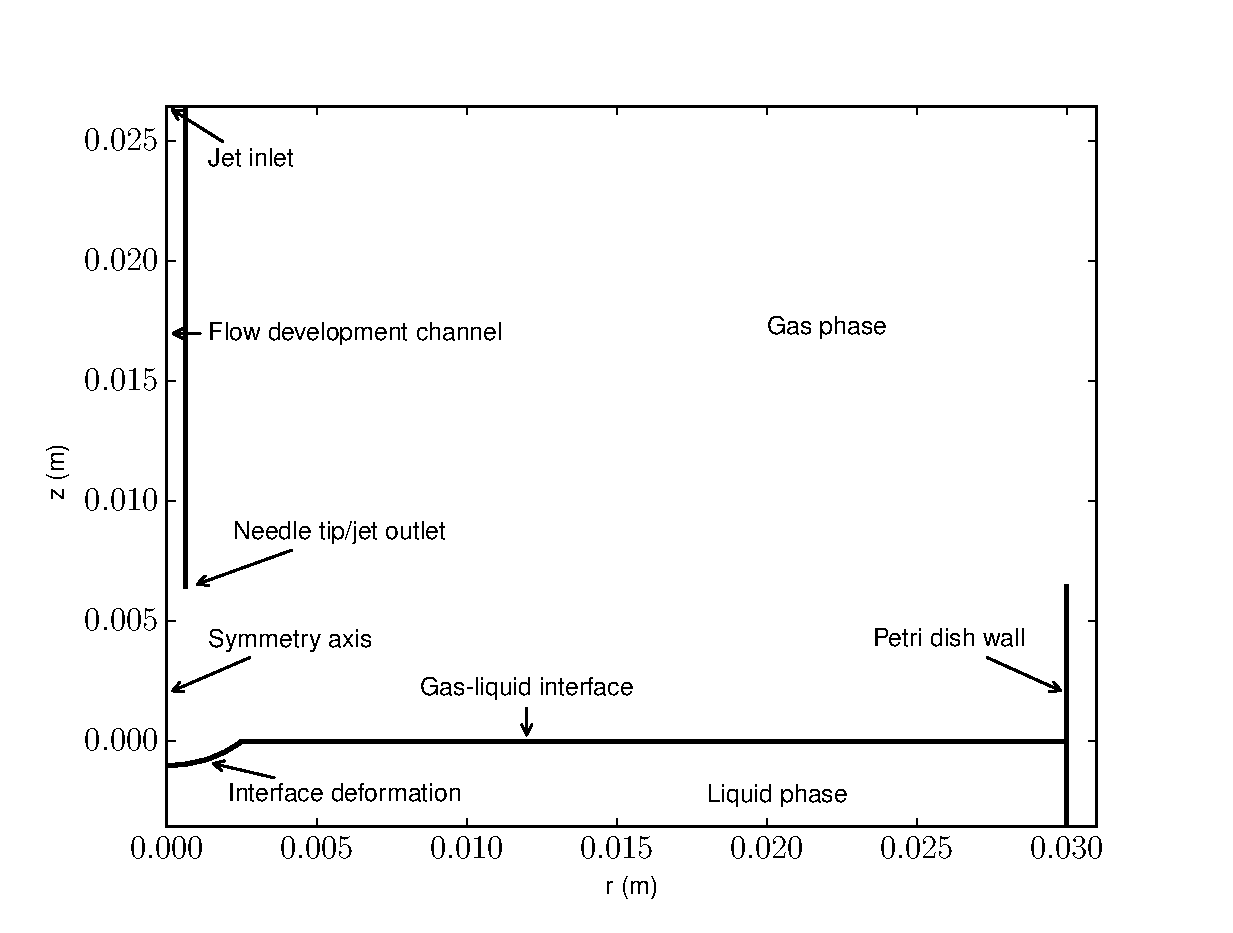
\includegraphics[width=\textwidth]{GeometryDeformed.eps}
    \caption{Geometry for deformed interface simulations.}
    \label{fig:deformed_geom}
\end{figure}

\begin{figure}[htb]
    \centering
    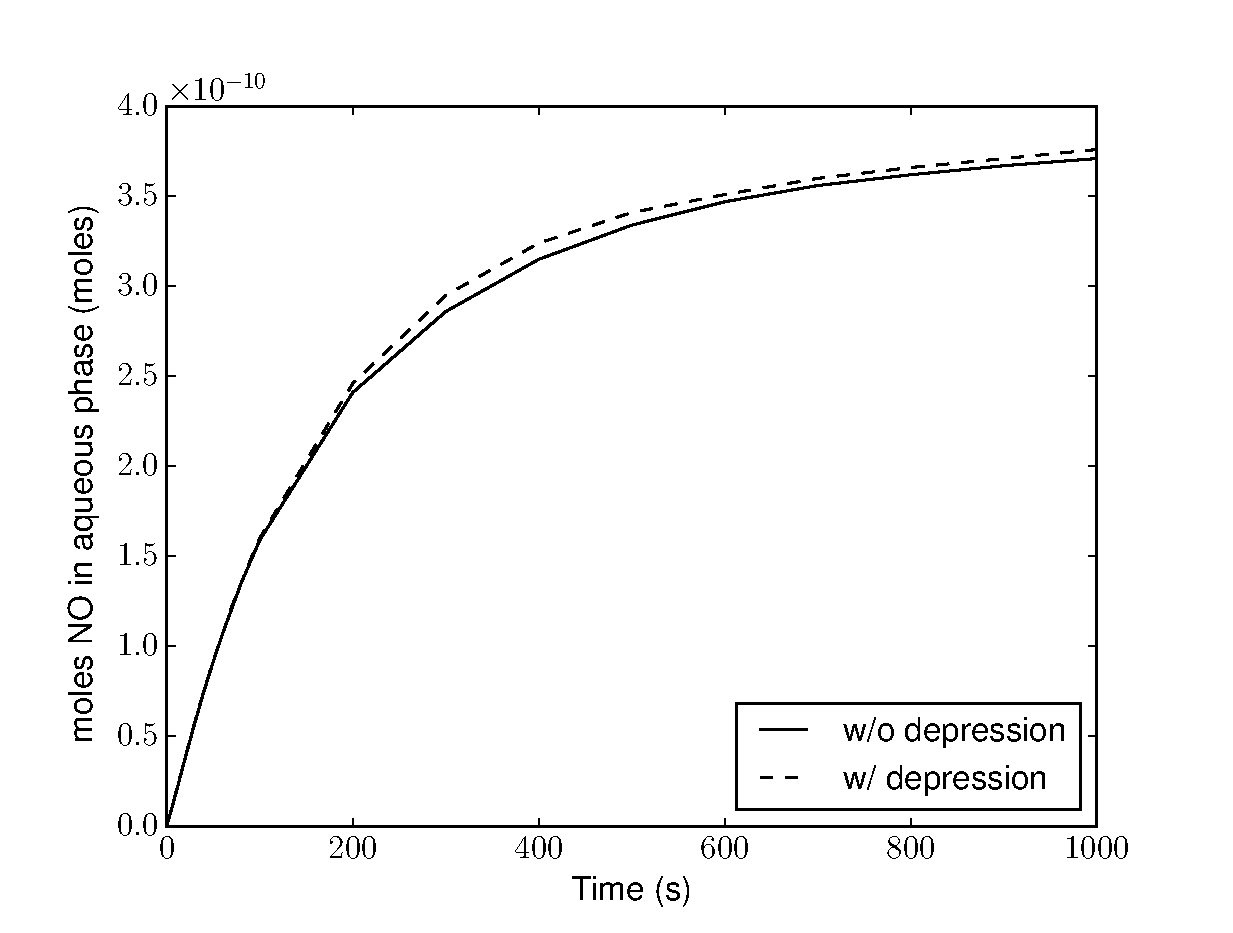
\includegraphics[width=\textwidth]{NO_dimple_plot.eps}
    \caption{Comparison of total NO(aq) uptake as a function of time for cases in which interface deformation is included and not included. As shown in the figure, the interface deformation has very little effect on the macrosocpic NO uptake. The effect for hydrophilic species is expected to be even less}
    \label{fig:NO_deform_compare}
\end{figure}

Before concluding, it is worth touching on the assumption of a flat interface. This work discusses the role gas phase convection plays in determining momentum, heat, and mass transport across a gas-liquid interface and into the bulk liquid. Species uptake is used as the criteria for determining whether to include self-consistent deformation of the interface by the gas flow. To make this determination, the shape of the interface deformation was observed experimentally and the deformation was introduced into the model geometry as shown in figure \ref{fig:deformed_geom}. The depth of the deformation was supported by a calculation balancing gravitational ($\rho$gh) and convective ($\frac{1}{2}\rho$v$^2$) stresses. The fluid flow simulation was then run until it reached stead-state, and then the heat and mass transfer equations were solved. In this way, though the interface deformation was not self-consistently determined, its influence on variables of interest could be analyzed. Shown in \ref{fig:NO_deform_compare} is the effect of the interface deformation on total solution uptake of NO(aq). As can be seen in the figure, the effect is minute. Because of the characteristics shown in Figure \ref{fig:excel}, the effect of the interface deformation on hydrophilic species transport is expected to be even less. Subsequently, for the purpose of this work, the interface deformation can be safely neglected.

Though comprehensive in many respects, the model in this section is not near complete without simulation of plasma discharge physics. Incorporating discharge physics requires changing simulation platforms from Comsol to Zapdos, a highly customizable code built by the authors where near total control over solution of the highly-nonlinear plasma equations is maintained. Zapdos is described in detail in \cref{chap:zapdos}. The 1D simulation effort in \cref{sec:plasliq} are the authors' first foray into self-consistent discharge-liquid modelling. Along with exploring questions about interfacial parameters, the work in \cref{sec:plasliq} is absolutely necessary for extending the work in this section. Combining the two modelling efforts is definitely on the roadmap for future work.

\FloatBarrier

\section{Fully Coupled Simulation of the Plasma Liquid Interface and Interfacial Coefficient Effects}
\label{sec:plasliq}

\subsection{Model Description}
\label{sec:model}
../plasmaliq_paper/model_description.tex
\FloatBarrier

\subsection{Results and Discussion}
\label{sec:plasliq_results}
../plasmaliq_paper/results_discussion.tex

% Figures to add text for:

\begin{figure}[htpb]
  \centering
  \includegraphics[width=.75\textwidth]{dummy_PowerDep_em.eps}
  \caption{Power deposited in electrons near the interface as a function of the interfacial surface loss coefficient}
  \label{fig:powerDep_em_int}
\end{figure}

\Cref{fig:powerDep_em_int} shows the power deposited into electrons from joule heating over the last 100 $\mu$m of the gas domain. It is evident that there is significantly more heating of the electrons for the higher reflection cases. This is almost entirely attributable to the enhanced electric field in the region (\cref{fig:efield_int}) that develops because of the build-up in negative charge density (\cref{fig:charge_dens_int}) from electron reflection. The electron current itself does not change with reflection as evidenced in \cref{fig:currents}.

\begin{figure}[htpb]
  \centering
  \includegraphics[width=.75\textwidth]{InterfacialChargeDensity.eps}
  \caption{Charge density near the interface as a function of the interfacial surface loss coefficient}
  \label{fig:charge_dens_int}
\end{figure}

\begin{figure}[htpb]
  \centering
  \includegraphics[width=.75\textwidth]{ElectronIonPowerDepFullGasDomain.eps}
  \caption{Power deposited in ions and electrons over the whole gas domain for low and high reflection cases}
  \label{fig:powerDep_em_Arp_full}
\end{figure}

Power deposition into both electrons and ions for the cases of $\gamma_{dens}=1$ and $\gamma_{dens}=10^{-4}$ are shown in \cref{fig:powerDep_em_Arp_full}. Ion power deposition profiles are identical between the different reflection cases. As expected for a DC discharge, all of the ion power deposition occurs in the cathode fall where both the electric field and ion current are significantly higher than in the bulk. Electron heating occurs throughout the discharge with local maxima in both the cathode and anode regions.

\begin{figure}[htpb]
  \centering
  \includegraphics[width=.75\textwidth]{RateProcesses.eps}
  \caption{Rate of ionization, excitation, and elastic collisions in the plasma for low and high reflection cases}
  \label{fig:rateProc}
\end{figure}

\Cref{fig:rateProc} shows the rate of elastic, excitation, and ionization collisions in the discharge. Elastic collision rates show an inverse relationship to the electron temperature: in the cathode where the electron temperature peaks, the elastic collision rate crashes; in the anode for the high reflection case ($\gamma_{dens}=10^{-4}$) the elastic collision rate peaks sharply because of the sharp fall in the electron temperature. Excitation collision rates are uniform through the bulk of the discharge for both high and low reflecion cases. Ionization rates peak in the bulk-sheath interface regions where the electron temperature is highest. Both excitation and ionization rates collapse in the cathode where electrons have not had sufficient time to gain energy; for high electron reflection the excitation and ionization rates also collapse in the anode.

\begin{figure}[htpb]
  \centering
  \includegraphics[width=.75\textwidth]{Currents.eps}
  \caption{Plot of specie and total currents in gas and liquid phases for low and high reflection cases}
  \label{fig:currents}
\end{figure}

\Cref{fig:currents} is a somewhat busy figure. It illustrates the currents carried by different species in gas and liquid phases as well as the total current. Dotted lines indicate the total current, solid lines the electron current, and dashed lines the argon and hydroxyl currents in the gas and liquid phases respectively. The curves do not show a strong functional dependence on the surface loss coefficient $\gamma_{dens}$. Current is carried by argon ions in the cathode, transitioning to electrons in the gas bulk and through the gas-liquid interface. As electrons react with water molecules, OH$^-$ becomes the dominant liquid current carrier away from the interface.

\begin{figure}[htpb]
  \centering
  \includegraphics[width=.75\textwidth]{ElectronFluxesBothDomains.eps}
  \caption{Breakdown of electron diffusive and advective fluxes in both domains for low and high reflection cases}
  \label{fig:electron_fluxes}
\end{figure}

Electron total, advective, and diffusive fluxes are illustrated in \cref{fig:electron_fluxes}. Consistent with \cref{fig:currents}, the total electron current rises from zero at the cathode to a constant value that it maintains through the gas bulk to the interface. The total current declines in the liquid phase because of electron reactions with H$_2$O. Advection and diffusion flux profiles are very similar between high and low reflection cases with the exception of the behavior very near the gas-liquid interface. Advective flux builds in the cathode until reaching a peak at the sheath-bulk interface. The advective flux then gradually declines in the bulk because of a gradual decrease in the bulk electric field until plummeting sharply in the anode as the electron density plummets; however, for the high reflection case very near the gas-liquid interface the advective flux rebounds sharply. This counter-acts the very strong leftward diffusive flux that arises from the large build-up in electron concentration. The net effect is that the total electron flux remains constant.

\section{Summary}

This chapter addresses a couple of fundamental questions regarding plasma-liquids. A qualitative study of the momentum, heat, and mass transport in a convective plasma-liquid system has been conducted in \cref{sec:plasfree_model}. Several interesting results were found. Convective flow of water vapor away from the interface leads to a sharp temperature gradient between the bulk gas and liquid phases. This sharp gradient is important for accurately determining temperature-dependent rate coefficients in both the gas and liquid phases. Additionally, convection drives water vapor away from the discharge region except immediately above the liquid surface; this could have important consequences for gas-phase generation of reactive species that depend on water as a precursor. Induced convection in the liquid phase substantially changes the spatial distribution of aqueous species and increases the volume-averaged uptake of hydrophobic species but interestingly has little effect on the volume-averaged uptake of hydrophilic species. This phenomena occurs because the majority of resistance to interfacial transfer is in the gas phase for hydrophilic species and in the liquid phase for hydrophobic species; consequently, decreasing the liquid-phase mass transfer resistance by adding liquid convection has a significant impact for hydrophobic but not for hydrophilic molecules.

Perhaps the most interesting result of the study in \cref{sec:plasfree_model} is the sharp distinction between reactivity at the surface and in the liquid bulk. Though the limited penetration (tens of $\mu$m or less) of reactive neutral radicals is well publicized in prominent biochemistry texts like \cite{Halliwell}, this phenomena has yet to receive significant attention in the plasma-liquid literature with the exception of \cite{Chen2014a}. Concentrations of species of interest for plasma-medicine and other applications (e.g. OH, NO, ONOOH) fall by as many as 9 orders of magnitude within 50 $\mu$m of the interface. In a relatively pure aqueous solution as is modeled here, the process responsible for conveying plasma reactivity to a target may be transport of H$_2$O$_2$ and acidified nitrite followed by a close-proximity reaction to form ONOOH and then OH and NO$_2$. For targets in aqueous biological systems, the conveyors of reactivity may be proteins modified by primary plasma species. What can be stated from the results presented here and in \cite{Chen2014a} is that these conveyors of plasma reactivity are probably not neutral radicals generated directly by the plasma; rather they are likely species generated by secondary reactions in the aqueous medium or more stable compounds like H$_2$O$_2$ and nitrite. To address this problem with even greater precision and detail, future research will involve developing a configuration-specific plasma and electrodynamics model that can be self-consistently coupled to the momentum, heat, and neutral species mass transport presented in this study.

The latter half of the chapter explores the fully self-consistent coupling of discharge physics with the liquid phase. The effects of varying unknown interfacial coefficients like $\gamma_{dens}$ and $\gamma_{en}$ are investigated. It is found that varying these parameters within reason can lead to interfacial gas-phase electron densities varying by orders of magnitude. The interfacial electron energy is also a very sensitive function of the interfacial parameters. This variation of electron density and energy could have significant impacts on both gas and liquid phase chemistry, thus our work motivates future studies to accurately determine the interfacial parameters. It is noteworthy that the overall potential drop and total current are relatively unaffected by changing gas-liquid interfacial parameters.

Self-consistently coupling the liquid domain to the highly non-linear plasma discharge equations as is done for \cref{sec:plasliq} requires an efficient multi-physics code. Comsol, the package used for the simulations in the first half of \cref{chap:basic_science}, has typically struggled to efficiently solve plasma problems. Thus a new code, named Zapdos, was built on top of the MOOSE framework for the express purpose of plasma-liquid simulations (although the highly modular nature of the code makes it easily extensible to other low-temperature plasma problems). The structure of Zapdos is the subject of \cref{chap:zapdos}.

\chapter{ZAPDOS: A TOOL FOR FULLY COUPLED MODELLING OF PLASMA-LIQUID SYSTEMS}
\label{chap:zapdos}

In \cref{chap:basic_science} we introduced two models addressing various aspects of plasma-liquids. In \cref{sec:plasfree_model}, we addressed momentum, heat, and neutral species transport using a 2D-axisymmetric model without explicity simulating the plasma discharge. In \cref{sec:plasliq} we examined the discharge physics coupled to the liquid phase in one dimension. The former model was created with the commercially available multi-physics package Comsol. However, efficient solution of the discharge governing equations coupled with liquid phase required creation of a novel plasma-simulation code, Zapdos, based on top of the Multiphysics Object-Oriented Simulation Environment (MOOSE). Creation of the fully-coupled plasma-liquid simulation environment is detailed in this chapter. In \cref{sec:zapdos} we describe Zapdos, the application physics code. In \cref{sec:moose} we detail changes implemented in the MOOSE framework allowing physics coupling across domains like that encountered in plasma-liquids.

\section{Zapdos Code}
\label{sec:zapdos}

\subsection{Zapdos Intro}
\label{sec:zapdos_intro}

It is perhaps prudent to warn the reader that the following subsection contains an overview of a lot of mathematics. We feel that this overview is worthwhile, however, for a couple of reasons. Firstly, the MOOSE application programmer principally responsible for providing two functions in his code: residuals and Jacobians. The following overview defines the meaning and importance of residuals and Jacobians in a physics simulation context. Secondly, the overview should give the reader an idea of the stunning level of control available to the MOOSE application programmer as he assembles and solves his physical simulation. We do not see it this way, but the high degree of control can be regarded as a two-edged sword. Building an accurate and efficient physical simulation on top of the MOOSE framework demands a level of understanding of the underlying mathematics well beyond that of a user of commercial multi-physics software. A minimum of a few months is required before acquiring the knowledge needed to achieve any interesting modelling results. However, once the developer has invested the requisite time and effort, the return is substantial as hopefully demonstrated in \cref{sec:plasliq} and in the exciting possibilities for future research (\cref{chap:conclusion}).

Zapdos is built on top of the MOOSE \cite{mooseSite} and libMesh \cite{libmeshSite} codes. MOOSE employs finite element methods (FEM), either Continuous Galerkin, Discontinuous Galerkin, or a combination, to solve fully coupled systems of partial differential equations (PDEs). Physics may also be segregated using the MOOSE multi-app system. After using FEM to discretize the governing equations, MOOSE interfaces with the code PetSc \cite{petscSite} to solve the non-linear or linear system of algebraic equations, $\vec{F}(\vec{u})$, via some form of Newton's method, where $\vec{F}$ is the residual vector and $\vec{u}$ is the vector of unknowns. A block diagram showing the interplay between Zapdos, MOOSE, libMesh, PetSc, as well as meshing and visualization packages (discussed more in \cref{sec:zap_meshing,sec:zap_post}) is shown in \cref{fig:diagram_workflow}. We will outline briefly the concept of forming the residual in the context of the finite element method. Let us consider the following differential equation:

\begin{equation}
  \nabla\cdot-D\nabla u = s(\vec{r})
  \label{eq:example}
\end{equation}

where diffusion of species $u$ is balanced by a source term $s(\vec{r})$. We refer to \cref{eq:example} as the strong form of our reaction-diffusion example problem. For FEM we convert the problem to what is known as the weak form by multiplying by a test function $\psi_i$ and integrating over the whole domain. We also move all terms to the left-hand side (LHS) of the equation such that the right-hand side (RHS) becomes 0. Our problem now becomes:

\begin{equation}
  \int_{\Omega}\psi_i\nabla\cdot-D\nabla u\,dV - \int_{\Omega}\psi_is(x)\,dV = 0
  \label{eq:example_weak}
\end{equation}

where $\Omega$ represents the extent of the domain. The first term is then integrated by parts to gives us:

\begin{equation}
  \int_{\Omega}\nabla\psi_i\cdot D\nabla u\,dV - \int_{\partial\Omega}\psi_iD\nabla u \cdot \vec{n}\,dS -\int_{\Omega}\psi_is(x)\,dV = 0
  \label{eq:example_weak_parts}
\end{equation}

where $\partial\Omega$ represents the domain boundaries. Integrals over the domain, e.g. terms 1 and 3 in \cref{eq:example_weak_parts}, are written in Zapdos and MOOSE as kernel class objects. Integrals over domain boundaries are written as boundary condition class objects. We will discuss Zapdos class objects more shortly. To continue our development of FEM, we must discretize the problem, or in other words convert our integral-differential equation into an algebraic equation. We accomplish this by dividing the domain volume into individual elements and associating basis functions with different geometric aspects of the discretization. Division of the domain into elements is also referred to as meshing. An example of a two-dimensional mesh is shown in \cref{fig:mesh}, where the domain has been sub-divided into triangular elements. For a two-dimensional domain, basis functions can be associated with mesh elements, edges, or vertices; in three-dimensions: elements, faces, edges, and vertices. Most commonly, Zapdos uses a linear basis associated with mesh vertices; these basis functions are commonly referred to as linear Lagrange. We construct a basis function $\phi_j(x,y,z)$ for each vertex that exists on the mesh (j = 1, 2, ..., N where N is the number of vertices in the domain). The function $\phi_j$ has these important properties: it is equal to one on vertex $j$ with coordinates $(x_j,y_j,z_j)$ and zero on all other vertices. This is illustrated in \cref{fig:basis_function} for a vertex sitting at the intersection of four two-dimensional triangular elements.

\begin{figure}[htbp]
  \centering
  \includegraphics[width=\maxwidth{\textwidth}]{test.png}
  \caption{Block-diagram laying out simulation work-flow}
  \label{fig:diagram_workflow}
\end{figure}

\begin{figure}[htbp]
  \centering
  \includegraphics[width=\maxwidth{\textwidth}]{2d_mesh.png}
  \caption{An example two-dimensional mesh. The domain is sub-divided into triangular elements.}
  \label{fig:mesh}
\end{figure}

\begin{figure}[htbp]
  \centering
  \includegraphics{basis_function.png}
  \caption{Basis function $\phi_1$ associated with vertex one. Vertex one sits at the intersection of four triangular two-dimensional elements. Note that $\phi_1$ equals unity at $(x_1,y_1)$ and zero at all other vertices. Illustration taken from \cite{FlahertyFEA}}
  \label{fig:basis_function}
\end{figure}

The dependent variable $u$ is obtained by summing over the whole basis:

\begin{equation}
  u = \sum_{j=1}^Nu_j\phi_j(x,y,z)
  \label{eq:basis_sum}
\end{equation}

where $u_j$ is the value of u at vertex $j$. The set of $u_j's$ represent the degrees of freedom or the quantities to be solved for. It is worthwhile to note that in Galerkin FEM, which is the only method used in Zapdos, the following relationship exists between basis and test functions: $\phi_k=\psi_k$ for k = 1, 2, ..., N. Substitution of \cref{eq:basis_sum} into \cref{eq:example_weak_parts} yields

\begin{equation}
  \int_{\Omega}\nabla\psi_i\cdot D\nabla \sum_{j=1}^Nu_j\phi_j(x,y,z)\,dV - \int_{\partial\Omega}\psi_iD\nabla \sum_{j=1}^Nu_j\phi_j(x,y,z) \cdot \vec{n}\,dS -\int_{\Omega}\psi_is(x)\,dV = R_i \approx 0
  \label{eq:example_weak_final}
\end{equation}

where we have introduced the idea that our governing equations form residual statements ($R_i$) that we hope to eventually drive to zero. The first and second terms of \cref{eq:example_weak_final} arising from diffusion can be analytically integrated. To complete the transformation of \cref{eq:example_weak_final} into an algebraic equation, the source term integral is computed with numerical quadrature. MOOSE employs Guassian quadrature, which for a general integrand s(x), can be written as:

\begin{equation}
  \int_a^bs(x)\,dx = \frac{b-a}{2}\sum_{i=1}^nw_is\left(\frac{b-a}{2}x_i+\frac{a+b}{2}\right)
  \label{eq:quad}
\end{equation}

where the $w_i's$ and $x_i's$ are the quadrature weights and points respectively. Details of calculation of $w_i$ and $x_i$ are not important to our purpose here; it is enough to know the concept of how a general integral is converted into an algebraic expression. After numericall integrating \cref{eq:example_weak_final}, the resulting algebraic expression can be evaluated using an initial guess for the $u_j's$. This results in the initial residual, with the residual essentially representing how close the $u_j's$ are to satisfying the governing equations; a residual of zero would represent a numerically perfect solution. In practice, the initial guess may be far from the actual solution. To rectify this, Zapdos, through MOOSE's interface with PetSc, uses Newton's method to iterate the solution vector $\vec{u}$ towards the true solution. Newton's method derives from a Taylor expansion: \cite{knoll2004jacobian}:

\begin{equation}
  \vec{R}(\vec{u}_{k+1}) = \vec{R}(\vec{u}_k) + \tilde{R'}(\vec{u}_k)(\vec{u}_{k+1}-\vec{u}_k)+\text{higher-order terms}
  \label{eq:Newton_step1_deriv}
\end{equation}

where in our case $\vec{R}$ is the residual vector of length N and $\vec{u}$ is the solution vector, also of length N where N in our example problem is equal to the number of mesh vertices as well as the number of basis functions. The index $k$ denotes the $k^{th}$ iteration of the Newton solve. In a more general case we may be solving for multiple fields, e.g. in addition to a concentration variable $u$ we may be solving for a temperature variable $T$. In this more general case (still limiting ourselves to a linear Lagrange discretization), $\vec{R}$ and $\vec{u}$ will have dimension equal to the \# of mesh vertices times the \# of field variables with $\vec{u}$ comprised of $T_j's$ and $u_j's$. (Indices $j$ and $k$ should not be confused; $u_j$ is one scalar element of the solution vector $\vec{u}$; $\vec{u}_k$ is the $k^{th}$ iterate of the solution vector computed during the Newton solve.) Returning to \cref{eq:Newton_step1_deriv}, if we set the left-hand side to zero (our goal is always to drive $\vec{R}_{k+1}$ to zero) and neglect the higher-order terms we reproduce the strict Newton method:

\begin{equation}
  \tilde{J}(\vec{u}_k)\vec{\delta u}_k = -\vec{R}(\vec{u}_k)
  \label{eq:Newton}
\end{equation}
\begin{equation}
  \vec{u}_{k+1} = \vec{u}_k + \vec{\delta u}_k
  \label{eq:strict_Newton}
\end{equation}

where $\tilde{J}$ is the Jacobian matrix formed by taking the derivatives of the residual vector with respect to the solution vector (equivalent to $\tilde{R'}$ in \cref{eq:Newton_step1_deriv}).\cite{knoll2004jacobian}  We iterate with \cref{eq:Newton,eq:strict_Newton} until the norm of $\vec{R}$ is below some user-defined tolerance. Strict Newton is known to have locally quadratic convergence; e.g. if the initial guess is relatively close to the solution, Newton's method will converge quickly and with ease. \cite{dennis1996numerical} In practice, however, the initial guess may not be close the solution. In this case a globalization method is used to increase the rate of convergence. Line search and trust region methods are the most common techniques for globalization. The default globalization in MOOSE applications is a line search with cubic backtracking. In a line search, \cref{eq:strict_Newton} is modified by simply inserting a multiplicative factor $\lambda$ in front of $\vec{\delta u}_k$ as shown in \cref{eq:line_search}.

\begin{equation}
  \vec{u}_{k+1} = \vec{u}_k + \lambda\vec{\delta u}_k
  \label{eq:line_search}
\end{equation}

Determining $\lambda$ is the realm of the particular line search technique chosen. The cubic backtracking technique for chosing $\lambda$ that is used in all Zapdos simulations is described in detail in \cite{dennis1996numerical}. We will give a short summary here. For simplicity, let us consider minimizing the residual $R$ of one nonlinear equation with one degree of freedom, $u$. We use the index $k$ to denote the $k^{th}$ Newton iteration and we introduce the index $l$ to denote the $l^{th}$ attempt to select a good value for $\lambda$. Since Newton's method displays exceptional convergence when $u_k$ is sufficiently close to the true solution, the zeroth guess for $\lambda$ is always $\lambda_0 = 1$. If $\lambda_0$ does not yield a desirable result (see \cref{eq:stopping}, then $\lambda_1$ is determined through quadratic backtracking (for details see \cite{dennis1996numerical}). If $\lambda_1$ also fails, the line search algorithm has sufficient information to perform a cubic backtrack. Cubic backtracking has the benefit over quadratic backtracking of being able to minimize $R$ when $R$ has negative curvature in the vicinity of $u_k$. Cubic backtracking minimizes the equation:

\begin{equation}
  m_{cu}(\lambda_l) = a\lambda_l^3+b\lambda_l^2+J(u_k)\delta u_k\lambda_l+R(u_k)
  \label{eq:bt}
\end{equation}

where J is our one-dimensional Jacobian equal to $\frac{\partial R}{\partial u}$ and $\delta u_k$ is the full Newton step determined from \cref{eq:Newton}; $a$ and $b$ are given by: \cite{dennis1996numerical}

\begin{equation}
  \begin{bmatrix} a \\ b \end{bmatrix} = \frac{1}{\lambda_{l-1}-\lambda_{l-2}} \begin{bmatrix} \frac{1}{\lambda_{l-1}^2} & \frac{-1}{\lambda_{l-2}^2} \\ \frac{-\lambda_{l-2}}{\lambda_{l-1}^2} & \frac{\lambda_{l-1}}{\lambda_{l-2}^2} \end{bmatrix} \begin{bmatrix} R(u_k+\lambda_{l-1}\delta u_k) - R(u_k) - J(u_k)\delta u_k\lambda_{l-1} \\ R(u_k+\lambda_{l-2}\delta u_k) - R(u_k) - J(u_k)\delta u_k\lambda_{l-2} \end{bmatrix}
  \label{eq:dets_bt}
\end{equation}

The stopping criterion used for $\lambda$ is: \cite{dennis1996numerical}

\begin{equation}
  R(u_k+\lambda_l\delta u_k) \leq R(u_k) + \alpha\lambda_lJ(u_k)\delta u_k
  \label{eq:stopping}
\end{equation}

with $\alpha$ chosen to be some value between 0 and 1; the default in PetSc is $\alpha=10^{-4}$. When the criterion of \cref{eq:stopping} is met, then the solution $u$ is updated through \cref{eq:line_search}. \Cref{eq:stopping} essentially requires that the average rate of decrease in R when moving from from $u_k$ to $u_k+\lambda_l\delta u_k$ be some fraction of the initial rate of decrease in that direction. The combination of \cref{eq:Newton,eq:line_search} is properly called a quasi-Newton method since the full Newton step is not necessarily used to update the solution vector at each iteration. However, since a globalization method like the line search described above is always combined with \cref{eq:Newton} in Zapdos simulations and any other practical Newton implentation, we will drop the quasi- prefix for the remainder of this discussion.

The linear problem for determining $\delta u_k$, \Cref{eq:Newton}, may be solved through either direct or iterative methods. The details of these methods are not critical to understanding the work in this dissertation, so we will give only a brief summary of them here. A direct method like lower-upper decomposition works well for relatively small problems. However, larger problems, particularly problems in three dimensions, require iterative Krylov subspace methods to be feasible. \cite{heil2008solvers} The most common Krylov technique and the one used by default in Zapdos is the generalized minimum residual method (GMRES) with restart. GMRES is an Arnoldi-based method; its algorithm is given in \cite{saad1986gmres}. The option to restart the GMRES algorithm prevents the inherent problem that as the number of linear iterations $k$ increases, the number of multiplications required to solve the linear system increases by $\frac{1}{2}k^2N$ where N denotes the number of degrees of freedom being solved for. \cite{saad1986gmres} The GMRES algorithm only requires knowledge of matrix vector products to complete the iteration, e.g. the Jacobian solution vector product on the LHS of \cref{eq:Newton}, as opposed to individual elements of the matrix. \cite{knoll2004jacobian} This makes GMRES conducive for a class of methods known as Jacobian-free Newton-Krylov (JFNK) methods, which will be discussed more shortly. Convergence of iterative methods like GMRES tends to improve as the condition number of the matrix $\tilde{A}$ in the equation $\tilde{A}\vec{x} = \vec{b}$ decreases. The condition number can be decreased through a process called preconditioning. Right preconditioning solves the new problem: $\tilde{A}\tilde{P}^{-1}\tilde{P}\vec{x} = \vec{b}$; left preconditioning solves problem $\tilde{P}^{-1}(\tilde{A}\vec{x} - \vec{b}) = 0$. The preconditioning matrix $\tilde{P}$ is usually based on the matrix $\tilde{A}$ or in our case the Jacobian matrix $\tilde{J}=\tilde{A}$. In creating $\tilde{P}$, there is a balance to strike between the degree of conditioning and the computational cost of applying the preconditioner. Choosing $\tilde{P}=\tilde{J}$ results in a conditioned matrix $\tilde{P}^{-1}\tilde{J}=\tilde{I}$ with an optimal condition number of one; solving the resulting conditioned system will take only one iteration to converge. However, the cost of applying the preconditioner is at a maximum. In practice, $\tilde{P}$ is much more sparse than $\tilde{J}$ and can be formed through a variety of techniques. The default serial preconditioning method for iterative linear solutions with Zapdos is incomplete lower-upper factorization which is described in detail in \cite{dupont1968approximate} and \cite{saad1996iterative}. Other preconditioning techniques are more parallelizable including block-Jacobi, which only fills the diagonal elements of the preconditioning matrix; \cite{saad1996iterative} the domain decomposition technique, additive Schwarz, which operates under the principle of divide and conquer; \cite{saad1996iterative} and multi-grid methods that rely on mesh restriction and prolongation operators. \cite{knoll2004jacobian} We recommend consulting this passage's references for more details on the mentioned preconditioning techniques.

When analytic calculation of Jacobian elements becomes either impossible or impractical, the property that GMRES only requires knowledge of matrix-vector products as opposed to individual matrix elements becomes very useful. It allows the modeller to implement the Jacobian-free approximation: \cite{knoll2004jacobian}

\begin{equation}
  \tilde{J}\vec{v} \approx \frac{\vec{R}(\vec{u}+\epsilon\vec{v})-vec{R}(\vec{u})}{\epsilon}
  \label{eq:jacob_free}
\end{equation}

where $\epsilon$ is a finite-differencing parameter chosen by the modeller. Using this approximation, the elements of the Jacobian matrix are never explicitly formed, giving the algorithm its ``Jacobian-free'' moniker. Using JFNK, one achieves Newton-like nonlinear convergence without the need for computing or storing the true Jacobian. \cite{knoll2004jacobian} Through finite differencing of the residual, JFNK feels out the true Jacobian, generally giving better convergence than if a Newton-Krylov method is used in conjunction with an incomplete or incorrect user-provided Jacobian matrix. Although JFNK methods are sometimes referred to as ``matrix-free'' methods, this is somewhat of a misnomer. In practice JFNK almost always involves forming a preconditioning matrix since the linear solve is intrinsically iterative.

In the precending section, we have hopefully illustrated the generation and importance of residual and Jacobian statements in simulating our physical system. To summarize, residual statements are pieces of the physical governing equations cast in the weak form and discretized with the finite element method. The Jacobian matrix $\tilde{J}$ is composed of derivatives of the residuals with respect to the solution vector $\vec{u}$. A maximally efficient application code in terms of computational time will have a complete and correct set of Jacobian statements and will employ a Newton method globalized with a line search. Small problems with accurate Jacobians can be solved directly, via lower-upper factorization for example; however, higher-dimensional problems may require a preconditioned iterative method to solve the linear system in \cref{eq:Newton}. If developer time is at a premium or some residual derivatives cannot be computed analytically, some Jacobian statements can be omitted and the Jacobian-Free approximation of \cref{eq:jacob_free} can be used. While still efficient, this method displays slower convergence than if a fully analytic and accurate Jacobian is supplied. Thus, the low-temperature plasma application Zapdos supplies complete and correct Jacobian statements wherever ot can. As new physics are introduced into Zapdos, newly coded analytical Jacobians are compared against PetSc Jacobians formed through finite differencing of the residual statements to ensure accuracy. The one-dimensional simulations run in \cref{sec:plasliq} featured fully accurate Jacobians; as a result, Newton's method combined with a direct solve of the linear system displayed the best rate of convergence. New 2-D axisymmetric simulations not reported in this work feature boundary condition residuals with non-local integrals. The coding infrastructure required to implement the corresponding Jacobian functions does not currently exist in MOOSE. Since the Jacobian is not completely accurate in this case, direct Newton and preconditioned JFNK display comparable rates of convergence.

Having given an overview of the mathematics that Zapdos relies on, we will turn to its coding implementation. Zapdos partitions governing equation terms into individual pieces called kernels. Each kernel contains the residual and the corresponding Jacobian statements. Recall our diffusion-reaction example from \cref{eq:example,eq:example_weak,eq:example_weak_parts,eq:example_weak_final}. Let us consider the first term in \cref{eq:example_weak_parts}; the corresponding Zapdos code looks like:

\begin{lstlisting}[language=C++,caption = Example of residual and Jacobian function definitions, label = code:resid_jacob]
Real
CoeffDiffusionLin::computeQpResidual()
{
  // Computes the residual
  return -_diffusivity[_qp] * _grad_u[_qp] * _r_units * -_grad_test[_i][_qp] * _r_units;
}

Real
CoeffDiffusionLin::computeQpJacobian()
{
  // Computes the Jacobian
  return -_diffusivity[_qp] * _grad_phi[_j][_qp] * _r_units * -_grad_test[_i][_qp] * _r_units;
}
\end{lstlisting}

where \_diffusivity is the diffusion coefficient, \_u is our solution variable, \_phi and \_test represent the shape and test functions that we introduced above, and \_qp represent the positions of quadrature points used for numerical integration. By splitting governing equations in this way into individual terms/kernels, code reproduction is kept at a minimum; analagous terms can be used in many different settings, e.g. a ``diffusion'' term has the exact same mathematical form as a ``conduction'' or ``viscosity'' term and so the same kernel code can be used for all three physics cases. Material properties like mobilty and diffusivity are defined in a materials file separated from the kernel code. Material properties can be defined as constants, as functions of the solution variables, or as properties to be read from look-up tables. Through MOOSE, Zapdos provides an interface for linear, bilinear, and spline interpolation of material properties. Boundary conditions are available in ``Nodal'' and ``Integrated'' flavors. Nodal boundary conditions are dirichlet like conditions that are enforced strongly. Integrated boundary conditions are cast in the weak form and often arise from performing integration by parts on divergence terms in the governing equations.

As of commit f74bad6, Zapdos has the necessary kernels and boundary conditions for solving gas phase DC discharge fluid models as well as conventional convection-diffusion-reaction equations for dilute species in a fluid. (Zapdos uses the software ``git'' for version control. The commit ``hash'' f74bad6 is essentially a version number.) Another student is working on implementing RF plasma simulation capabilities (for capacitively coupled plasmas this will only require slight modification of some boundary conditions; inductively coupled plasmas will require a little more work). These efforts will be detailed further in \cref{chap:conclusion}.

Zapdos solutions are output to an exodus file by default, although MOOSE provides varying levels of support for some other output file formats (including full support for simple CSV). Exodus files are a file type developed at Sandia National Lab designed specifically for storing and retrieving finite element data. \cite{schoof1994exodus} These exodus files are most commonly viewed graphically with either of the open source packages Visit or Paraview. For users more programatically inclined, Paraview provides python tools that enable the user to directly read the exodus file and create publication level plots in MatPlotLib with a single script (as is done for a lot of figures in this dissertation). For transient simulations, results for any solution or auxiliary variable can be viewed while the calculation is on-line. Results are also not lost if a solve is cancelled for any reason. These features enable quick convergence debugging of a failing or failed solve.

Another feature of Zapdos is the adaptive mesh refinement inherited from MOOSE. The user can choose from several different indicators, including the jump in a solution gradient or laplacian between elements, for determing where mesh refinement should take place. Figures \ref{fig:step15} and \ref{fig:step49} show the results of an advection-diffusion simulation for temperature in which a pressure difference between the left and right ends of the domain induce bulk flow from left to right. The effective mobility of the temperature is specified to be greater in the bottom half of the domain, resulting in faster temperature flow in the bottom half. Note that the mesh is refined at the head of the temperature flow where numerical instabilities are more likely to occur; once the temperature front has passed the mesh is coarsened to reduce computational expense. This feature can be incredibly useful when trying to track ionization bullets (\cref{fig:bullets}) or similar phenomena.

\begin{figure}[htbp]
  \centering
  \includegraphics[width=.4\textwidth]{Time_step_15.eps}
  \caption{Propagating front. Time step 15. Note how the mesh is fine around the solution gradients and coarse elsewhere.}
  \label{fig:step15}
\end{figure}

\begin{figure}[htbp]
  \centering
  \includegraphics[width=.4\textwidth]{Time_step_49.eps}
  \caption{Propagating front. Time step 49. Note how the mesh is fine around the solution gradients and coarse elsewhere.}
  \label{fig:step49}
\end{figure}

\begin{figure}[htbp]
  \centering
  \includegraphics[width=\textwidth]{Ionization_bullets.png}
  \caption{Ionization bullets simulated with Zapdos. Mesh adaptivity is used to follow their propagation.}
  \label{fig:bullets}
\end{figure}

\subsection{Zapdos Kernels}
\label{sec:zap_kernels}

As mentioned in the introductory section, Zapdos takes each term in a governing equation and casts that term as a class with methods for computing the residual and Jacobian. These governing equation term classes are called kernels. As of commit f74bad6, Zapdos has 77 kernels. However, not all of these have utility, e.g. one kernel may have been re-cast as a new class without the old class being removed from the kernel directory. The most important kernels, e.g. the ones actively being used for physics and engineering research, are enumerated below. An important feature of Zapdos is the option to cast concentration or density variables in a logarithmic form, e.g. $N_k = \ln\left(n_k\right)$ where $N_k$ is the logarithmic variable representation of the density and $n_k$ is the true physical density. This is done for the modelling studies presented in \cref{sec:plasliq}. The advantage of the logarithmic casting is that it prevents the true concentration from ever becoming negative. Negative concentrations can be a product of and contribute to numerical instabilities. Negative concentrations can cause source terms to become sink terms and visa versa, thus it is advantageous to avoid them if possible.

Also for all the simulations described in \cref{sec:plasliq}, it is the logarithm of the \textit{product} of the electron density and mean energy that is a solution variable as opposed to simply the logarithm of the mean energy. Thus for the simplest plasma discharge simulation, there are four solution variables:

\begin{gather}\label{eq:soln_vars}
  N_i = \ln n_i\\
  N_e = \ln n_e\\
  E_n = \ln\left(n_e\epsilon\right)\\
  V = V
\end{gather}

where n$_i$ and n$_e$ are the physical ion and electron densities respectively, $\epsilon$ is the mean electron energy, and V is the potential. Anywhere that $n_i$ exists in the governing equations, it is replaced with $e^{N_i}$; $n_e$ is replaced with $e^{N_e}$; the product of $n_e$ and $\epsilon$ is replaced with $e^{E_n}$. Whatever units are used for the original variables are retained by their replacement expressions, e.g. if $n_e$ has units of \#/m$^3$ then the expression $e^{N_e}$ has units of \#/m$^3$. While the choice to use the product of n$_e$ and $\epsilon$ simplifies some parts of the governing equation, it complicates others. In particular the electron transport and Townsend coefficients that are functions of the mean electron energy become functions of two solution variables, N$_e$ and E$_n$, as opposed to just one. Thus residual/governing equation terms that involve electron transport or Townsend coefficients must include Jacobian contributions from both N$_e$ and E$_n$.

In order to improve conditioning of the Jacobian, Zapdos provides the user options for unit scaling. The potential can either be cast in units of volts or kilovolts (this will be made even more flexible in the future). This choice is made in the GlobalParams block of the Zapdos input file, by specifying $potential\_units = V$ or $potential\_units = kV$. The length units can also be scaled. In the coupled plasma-liquid simulations described in \cref{sec:plasliq}, the plasma domain length is 1 mm, whereas the water domain length is 100 nm. Thus at the beginning of the input file, in order to scale closer to unity, we specify $dom0scale = 1e-3$ and $dom1scale = 1e-7$. The values of $dom0Scale$ and $dom1Scale$ can then be accessed using the syntax, \$\{\}. \cite{GetPot} Thus for any kernel or boundary condition that contains a gradient term, we specify the parameter: $position\_units = \$\{dom0Scale\}$ or $position\_units = \$\{dom1Scale\}$ depending on whether the kernel or boundary condition is acting in the gas or liquid phase. Unlike the $potential\_units$ parameter which must be a string equal to $V$ or $kV$, the $position\_units$ parameter can be set to any real number. The length scaling is represented in \cref{tab:zap_kernels} as the symbol $l_c$ where $l_c$ is actually equal to $1/position\_units$; the potential scaling is represented by $V_c$ where $V_c=1000$ if $potential\_units=kV$ else $V_c=1$ if $potential\_units=V$.

Zapdos tries to be as generic and modular as possible in the formulation of its kernels, e.g. a diffusion kernel code should be as applicable to the diffusion of Argon ions in the gas phase as it is to neutral OH radicals in the liquid phase. However, advection-diffusion-reaction (ADR) terms for electrons in the plasma typically have to have their own kernels because the transport and Townsend coefficients are allowed to be functions of the mean electron energy as opposed to constants. In this case Jacobian terms must be provided for the coefficient functional dependence on both N$_e$ and E$_N$. This functional dependence does not exist when the coefficients are constant as in the cases where we are modelling transport of heavy ions and neutrals, thus those kernels can be completely generic. For generic kernels, the solution variable is denoted by $u$ in \cref{tab:zap_kernels}; a coupled solution variable is denoted by $v$. Note that the kernel residuals/governing equation terms are cast in the weak form, i.e. each term in the governing equation is multiplied by a test function $\psi_i$ where $i$ denotes the $i^{th}$ shape function. Divergence terms, e.g. flux terms, are integrated by parts to produce both a volumetric kernel term and a surface boundary condition term (or surface discontinuous Galerkin term if a discontinuous Galerkin discretization is used). $\mu$ is the mobility of the species the kernel is acting on, $D_k$ is the diffusivity, $l_c$ is the characteristic length defined in the paragraph above, $\alpha_{iz}$, $\alpha_{ex}$, and $\alpha_{el}$ are the Townsend ionization, excitation, and elastic collision coefficients respectively, $sgn(q)$ is the charge sign, $k$ is used to generally represent reaction coefficients, $N_A$ is Avogadro's number, and $e$ is the Coulombic charge equal to $1.6x10^{-19}$ C. All other symbols should be defined in their corresponding table entry.

\begin{ThreePartTable}
  \begin{TableNotes}
    %% \footnotesize
    \item [a] \(\displaystyle \vec{\Gamma_e} = \mu_e(N_e,E_n) \nabla V l_c e^{N_e} - D_e(N_e,E_n) e^{N_e} \nabla N_e l_c\)
  \end{TableNotes}

  \begin{longtable}{>{\centering}m{2.25in}| >{\centering}m{1.75in}| >{\raggedright\arraybackslash}m{1.5in}}
    \caption{Kernels in Zapdos used for simulations presented in \cref{sec:plasliq}} \label{tab:zap_kernels} \\\toprule
    \textbf{Kernel Name} & \textbf{Governing Eqn. Term}\tnote{a} & \textbf{Description}\\\hline\hline
    \endfirsthead
    \caption{Continued} \\\toprule
    \textbf{Kernel Name} & \textbf{Governing Eqn. Term}\tnote{a} & \textbf{Description}\\\hline\hline
    \endhead
    \endfoot
    \endlastfoot

    ElectronTimeDerivative & \(\displaystyle \psi_i e^u\frac{\partial u}{\partial t}\) & Generic accumulation term\\\hline
    EFieldAdvectionElectrons & \(\displaystyle -\nabla\psi_i \mu_e(N_e,E_n) e^{N_e}\nabla V /l_c^2\) & Electron specific electric field driven advection term\\\hline
    CoeffDiffusionElectons & \(\displaystyle \nabla\psi_i D_e(N_e,E_n) e^{N_e} \nabla N_e /l_c^2\) & Electron specific diffusion term\\\hline
    ElectronsFromIonization & \(\displaystyle -\psi_i \alpha_{iz}(E_n,N_e) \lvert\vec{\Gamma_e}\rvert\) & Rate of production of electrons from ionization\\\hline
    LogStabilizationMoles & \(\displaystyle -\psi_i e^{-(b+u)}\) & Kernel stabilizes solution variable $u$ in places where $u\rightarrow 0$; $b$ is the offset value specified by the user. A typical value for $b$ is 20.\\\hline
    EFieldAdvection & \(\displaystyle -\nabla \psi_i \mu\sgn(q) e^u \cdot -\nabla V /l_c^2\) & Generic electric field driven advection term\\\hline
    CoeffDiffusion & \(\displaystyle -\nabla \psi_i -D_e e^u \nabla u /l_c^2\) & Generic diffusion term\\\hline
    ReactantFirstOrderRxn & \(\displaystyle \psi_i k e^u\) & Generic first order reaction sink term for $u$ ($u$ is the reactant); $k$ is the reaction rate coefficient\\\hline
    ReactantAARxn & \(\displaystyle 2 \psi_i k e^{2u}\) & Generic second order reaction sink term for $u$ in which two molecules of $u$ are consumed\\\hline
    CoeffDiffusionLin & \(\displaystyle -\nabla \psi_i \cdot -D \nabla u /l_c^2\) & Generic \textit{linear} diffusion term, e.g. this is a diffusion term for solution variables \textit{not} cast in a logarithmic form\\\hline
    ChargeSourceMoles\_KV & \(\displaystyle \frac{-\psi_i e \sgn(q) N_A e^v}{V_c}\) & Used for adding charged sources to Poisson's equation; $e^v$ represents the charged particle density of species $v$. This kernel assumes that densities are measured in units of mol/volume as opposed to \#/volume.\\\hline
    IonsFromIonization & \(\displaystyle -\psi_i \alpha_{iz}(E_n,N_e) \lvert\vec{\Gamma_e}\rvert\) & Same governing term/residual as ElectronsFromIonization; however, the Jacobian structure is different. $\frac{\partial R_i}{\partial N_e}$ will be on-diagonal for ElectronsFromIonization and off-diagonal for IonsFromIonization\\\hline
    ProductFirstOrderRxn & \(\displaystyle -\psi_i k e^v\) & Generic first order reaction source term for $u$ ($v$ is the reactant)\\\hline
    ProductAABBRxn & \(\displaystyle -2\psi_i k e^{2v}\) & Generic second order reaction source term in which two molecules of $v$ are produced from two molecules of $u$\\\hline
    EFieldAdvectionEnergy & \(\displaystyle -\nabla \psi_i \mu_{\epsilon}(N_e,E_n) e^{E_n} \cdot \nabla V /l_c^2\) & Electron energy specific electric field driven advection term\\\hline
    CoeffDiffusionEnergy & \(\displaystyle -\nabla \psi_i \cdot -D_{\epsilon}(N_e,E_n) e^{E_n}\nabla E_n /l_c^2\) & Electron energy specific diffusion term\\\hline
    JouleHeating & \(\displaystyle -\psi_i \nabla V V_c /l_c \cdot \vec{\Gamma_e}\) & Joule heating term for electrons\\\hline
    ElectronEnergyLossFromIonization & \(\displaystyle \psi_i \alpha_{iz}(N_e,E_n)\lvert\vec{\Gamma_e}\rvert E_{iz}\) & Electron energy loss term for inelastic ionization collisions; $E_{iz}$ is the energy lost in Volts in a single ionization collision\\\hline
    ElectronEnergyLossFromExcitation & \(\displaystyle \psi_i \alpha_{ex}(N_e,E_n)\lvert\vec{\Gamma_e}\rvert E_{ex}\) & Electron energy loss term for inelastic excitation collisions; $E_{ex}$ is the energy lost in Volts in a single excitation collision\\\hline
    ElectronEnergyLossFromElastic & \(\displaystyle \psi_i \alpha_{el}(N_e,E_n)\lvert\vec{\Gamma_e}\rvert \frac{3m_eT_e}{m_n}\) & Electron energy loss term for elastic collisions. $\alpha_{el}$ is the elastic Townsend coefficient; $m_e$ is the electron mass; $m_n$ is the mass of the neutral background gas; $T_e = \frac{2\epsilon}{3}$ is the electron temperature\\\hline
    \insertTableNotes
  \end{longtable}
\end{ThreePartTable}

\subsection{Zapdos Auxiliary Kernels}
\label{sec:zap_aux}

Zapdos implements a variety of auxiliary kernels that, while not essential to the solve, are important for visualizing and understanding the plasma-liquid physics. The auxiliary kernels that are employed for the simulations in \cref{sec:plasliq} are outlined in \cref{tab:aux_kernels}.

\begin{ThreePartTable}
  \begin{TableNotes}
    %% \footnotesize
    %% \item [a]
  \end{TableNotes}

  \begin{longtable}{>{\centering}m{2in}| >{\centering}m{2in}| >{\raggedright\arraybackslash}m{1.5in}}
    \caption{AuxKernels in Zapdos used for visualization of simulation results described in \cref{sec:plasliq}}\label{tab:aux_kernels}\\\toprule
    \textbf{AuxKernel Name} & \textbf{Expression} & \textbf{Description}\\\hline\hline
    \endfirsthead
    \caption{Continued}\\\toprule
    \textbf{AuxKernel Name} & \textbf{Expression} & \textbf{Description}\\\hline\hline
    \endhead
    \endfoot
    \endlastfoot

    PowerDep & \(\displaystyle \sgn(q)e N_A\cdot(\sgn(q)\mu\cdot-\nabla V e^{N_k} - D e^{N_k} \nabla N_k) \cdot -\nabla V V_c/l_c^2\) & Amount of power deposited into a user specified specie by Joule Heating\\\hline
    ProcRate & \(\displaystyle N_A \cdot \abs{-\mu_e\cdot-\nabla V e^{N_e} - D_e e^{N_e} \nabla N_e} \cdot \alpha /l_c\) & Reaction rate for electron impact collisions in units of $\frac{\#}{m^3s}$. User can pass choice of elastic, excitation, or ionization\\\hline
    ElectronTemperature & \(\displaystyle \frac{2}{3}e^{E_n-N_e}\) & The electron temperature\\\hline
    Position & \(\displaystyle x l_c\) & Produces an elemental auxiliary variable useful for plotting against other elemental auxiliary variables. Mesh points automatically output by Zapdos only work for plotting nodal variables. Since almost all auxiliary variables are elemental, this AuxKernel is very important.\\\hline
    Density & \(\displaystyle e^{N_k} N_A\) & Returns physical densities in units of $\frac{\#}{m^3}$\\\hline
    Efield & \(\displaystyle -\nabla V / l_c\) & Returns the x-component of the electric field (only relevant component for 1-D simulations)\\\hline
    Current & \(\displaystyle \sgn(q_k) e N_A \cdot(\sgn(q)\mu_k\cdot-\nabla V e^{N_k} / l_c - D_k e^{N_k} \nabla N_k / l_c)\) & Returns the electric current associated with the flux of species $k$\\\hline
    EFieldAdvAux & \(\displaystyle \sgn(q_k)\mu_k e^{N_k} \cdot -\nabla V N_A / l_c\) & Returns the electric field driven advective flux of species $k$\\\hline
    DiffusiveFlux & \(\displaystyle -D_k e^{N_k} \nabla N_k N_A / l_c\) & Returns the diffusive flux of species $k$\\\hline
  \end{longtable}
\end{ThreePartTable}

\subsection{Zapdos Interface Kernels}
\label{sec:zap_interface}

Critical to fully coupling the plasma and liquid phase simulations are the conditions at the interface. Initially, it was not possible to create interfacial conditions in Zapdos because the capability did not exist in the MOOSE framework. However, as described in \cref{sec:moose}, we were able to add the capability to the framework, and thus it is now possible to create interfacial conditions in Zapdos. A couple important ones that are used in mean\_en.i (see \cref{sec:zap_input}) are described in \cref{tab:interface}.

\begin{ThreePartTable}

  \begin{TableNotes}
  \end{TableNotes}

  \begin{longtable}{>{\centering}m{2in}| >{\centering}m{1.75in}| >{\raggedright\arraybackslash}m{1.75in}}
    \caption{Important InterfaceKernels in Zapdos} \label{tab:interface} \\\toprule
    \textbf{InterfaceKernel Name} & \textbf{Expression} & \textbf{Description}\\\hline\hline
    \endfirsthead
    \caption{Continued}\\\toprule
    \textbf{InterfaceKernel Name} & \textbf{Expression} & \textbf{Description}\\\hline\hline
    \endhead
    \endfoot
    \endlastfoot

    InterfaceAdvection & \(\displaystyle -\psi_{i,el}\mu_{k,n}\sgn(q_k) e^{N_{k,n}}\nabla V_n \cdot \vec{n} / (l_{c,n}l_{c,el})\) & Used to include the electric field driven advective flux of species $k$ into or out of a neighboring subdomain. The subscript $el$ denotes the subdomain to which the InterfaceAdvection residual is being added. The subscript $n$ denotes the neighboring subdomain. Currently this interface kernel is specific to electrons because the transport coefficients are assumed to be a function of the mean electron energy. A generic interface kernel with constant transport coefficients will have a much simpler Jacobian\\\hline
    InterfaceLogDiffusionElectrons & \(\displaystyle -\psi_{i,el} D_{k,n} e^{N_{k,n}} \nabla N_{k,n} \cdot \vec{n} / (l_{c,n}l_{c,el})\) & Used to include the diffusive flux of species $k$ into or out of a neighboring subdomain. Also currently specific to electrons.\\\hline
  \end{longtable}
\end{ThreePartTable}

\subsection{Zapdos Boundary Conditions}
\label{sec:zap_bcs}

Zapdos boundary conditions at the cathode are based on the work in \cite{hagelaar2000boundary} and \cite{sakiyama2007nonthermal}. For ions, electrons, and the electron energy, the most commonly used conditions are respectively (in strong form and without scaling factors):

\begin{equation}
  \vec{\Gamma_i}\cdot\vec{n} = \frac{1-r_i}{1+r_i}\left(\left(2a_i-1\right)\mu_i\vec{E}\cdot\vec{n}n_i + \frac{1}{2}v_{th,i}n_i\right)
  \label{eq:ion_bc_3}
\end{equation}
\begin{equation}
    \vec{\Gamma_e}\cdot\vec{n} = \frac{1-r_{dens}}{1+r_{dens}}\left(-\left(2a_e-1\right)\mu_e\vec{E}\cdot\vec{n}\left(n_e-n_{\gamma}\right) + \frac{1}{2}v_{th,e}\left(n_e-n_{\gamma}\right)\right) - \left(1-a_e\right)\gamma_p\vec{\Gamma_p}\cdot\vec{n}
  \label{eq:electron_bc_3}
\end{equation}
\begin{equation}
    \vec{\Gamma_{\epsilon}}\cdot\vec{n} = \frac{1-r_{en}}{1+r_{en}}\left(-\left(2a_e-1\right)\frac{5}{3}\mu_e\vec{E}\cdot\vec{n}\left(n_e\epsilon-n_{\gamma}\epsilon_{\gamma}\right) + \frac{5}{6}v_{th,e}\left(n_e\epsilon-n_{\gamma}\epsilon_{\gamma}\right)\right) - \frac{5}{3}\epsilon_{\gamma}\left(1-a_e\right)\gamma_p\vec{\Gamma_p}\cdot\vec{n}
  \label{eq:energy_bc_3}
\end{equation}

where $r_i$, $r_{dens}$, $r_{en}$ are the boundary reflection coefficients for ions, electrons, and electron energy respectively (more discussion on $r_{en}$ shortly), $\gamma_p$ is the secondary electron emission coefficient, $\epsilon_{\gamma}$ is the energy of the secondary electrons, $\vec{n}$ is the outward facing normal vector, and:

\begin{equation}
  a_k =
    \begin{cases}
      1, & sgn_k\mu_k\vec{E}\cdot\vec{n}>0 \\
      0, & sgn_k\mu_k\vec{E}\cdot\vec{n}\leq0
    \end{cases}
  \label{eq:a_3}
\end{equation}
\begin{equation}
  v_{th,k} = \sqrt{\frac{8T_k}{\pi m_k}}
  \label{eq:v_th_3}
\end{equation}
\begin{equation}
  n_{\gamma} = \left(1-a_e\right)\frac{\gamma_p\vec{\Gamma_p}\cdot\vec{n}}{\mu_e\vec{E}\cdot\vec{n}}
  \label{eq:n_gamma_3}
\end{equation}

where $v_{th,k}$ is the thermal velocity of species $k$ and $n_{\gamma}$ is the density of secondary electrons. A thermodynamic interfacial condition is also available:

\begin{equation}
  Hn_{e,g} = n_{e,l}
  \label{eq:electron_bc_thermo_3}
\end{equation}

For ions and electrons in the liquid phase, depending on the polarity of the discharge, a simple outflow BC is used at the counter electrode at the bottom of the liquid. Its strong form is:

\begin{equation}
  \vec{\Gamma_k}\cdot\vec{n} = -a_k \mu_k \sgn(q_k) e^{N_k} \nabla V \cdot \vec{n}
  \label{eq:outflow_3}
\end{equation}

For potential conditions, grounding is done using a DirichletBC class inherited from MOOSE. The other boundary condition incorporates an external ballast resistor:

\begin{equation}
  V_{source} + V_{cathode} = \left(e\vec{\Gamma_i} - e\vec{\Gamma_e}\right)AR
  \label{eq:cathode_3}
\end{equation}

A summary of the important boundary condition classes that Zapdos defines are summarized in \cref{tab:bcs}.

\begin{ThreePartTable}

  \begin{TableNotes}
  \end{TableNotes}

  \begin{longtable}{>{\centering}m{2in}| >{\centering}m{2in}| >{\raggedright\arraybackslash}m{1.5in}}
    \caption{Important BoundaryConditions defined by Zapdos} \label{tab:bcs}\\\toprule
    \textbf{BoundaryCondition Name} & \textbf{Expression (strong form and without scaling factors)} & \textbf{Description}\\\hline\hline
    \endfirsthead
    \caption{Continued}\\\toprule
    \textbf{BoundaryCondition Name} & \textbf{Expression (strong form and without scaling factors)} & \textbf{Description}\\\hline\hline
    \endhead
    \endfoot
    \endlastfoot

    HagelaarIonAdvectionBC & First parenthetical term in \cref{eq:ion_bc_3} & Kinetic advective ion boundary condition\\\hline
    HagelaarIonDiffusionBC & Second parenthetical term in \cref{eq:ion_bc_3} & Kinetic diffusive ion boundary condition\\\hline
    HagelaarElectronBC & \cref{eq:electron_bc_3} & Kinetic electron boundary condition\\\hline
    HagelaarEnergyBC & \cref{eq:energy_bc_3} & Kinetic electron energy boundary condition\\\hline
    DCIonBC & \cref{eq:outflow_3} & Electric field driven outflow boundary condition\\\hline
    NeumannCircuitVoltageMoles\_KV & \cref{eq:cathode_3} & Circuit boundary condition for potential\\\hline
    MatchedValueLogBC & \cref{eq:electron_bc_thermo_3} & Henry's Law like thermodynamic boundary condition for specifying a specie concentration ratio at the gas-liquid interface\\\hline
  \end{longtable}
\end{ThreePartTable}

\subsection{Zapdos Materials}
\label{sec:zap_materials}

Transport, rate, and other properties are defined in class files in the materials directory of Zapdos. Gas properties (whether argon, air, etc.) are defined in the class file Gas.C. Aqueous solute properties are defined in the class file Water.C. In the gas phase, electron transport and Townsend rate coeffiecients are functions of the electron mean energy (or alternatively they can be functions of the local electric field). As shown in \cref{code:read_in}, this data is read in from a whitespace-delimited look-up table from a text input file. The look-up table data is parsed into interpolation objects. There are several interpolation types that MOOSE application developers can choose from; we have chosen to use a spline interpolator. Because a spline interpolator provides C$^2$ continuity, there are no derivative jumps with respect to the mean energy. This in turn makes for continuous Jacobian functions, leading to markedly improved convergence over a linear interpolator for example.

\begin{lstlisting}[language=C++, caption = Code for reading in electron transport and Townsend coefficient data from a lookup table in a text file, label = code:read_in]
  // Define path to look-up table
  std::string tdPath = "/src/materials/td_argon_mean_en.txt";
  std::string path = zapDir + tdPath;
  const char *charPath = path.c_str();

  // Create input file stream: myfile
  std::ifstream myfile (charPath);
  Real value;

  if (myfile.is_open())
  {
    // As long we haven't reached the end of file, read entries from the look-up table into respective data arrays
    while ( myfile >> value )
    {
      // Get mean energy values that Townsend and transport coefficients are a function of
      actual_mean_energy.push_back(value);
      myfile >> value;
      // Townsend ionization coefficient
      alpha.push_back(value);
      myfile >> value;
      // Townsend excitation coefficient
      alphaEx.push_back(value);
      myfile >> value;
      // Townsend elastic collision coefficient
      alphaEl.push_back(value);
      myfile >> value;
      // Electron mobility
      mu.push_back(value);
      myfile >> value;
      // Electron diffusivity
      diff.push_back(value);
    }
    myfile.close();
  }

  else std::cerr << "Unable to open file" << std::endl;

  // Create interpolation functions for Townsend and transport coefficients that depend on the mean energy
  _alpha_interpolation.setData(actual_mean_energy, alpha);
  _alphaEx_interpolation.setData(actual_mean_energy, alphaEx);
  _alphaEl_interpolation.setData(actual_mean_energy, alphaEl);
  _mu_interpolation.setData(actual_mean_energy, mu);
  _diff_interpolation.setData(actual_mean_energy, diff);
\end{lstlisting}

\Cref{code:mat_def} shows definition of both constant material properties and solution variable-dependent properties. In this particular codeblock the code tests whether the user wants the electron mobility and diffusivity to be functions of the mean energy. If so, the interpolator \textbf{sample} method is called to retrieve the property at the corresponding value for the mean energy (recall that $\epsilon$ is a function of $E_n$ and $N_e$; see \cref{eq:soln_vars}). In addition the interpolator's \textbf{sampleDerivative} method is also called; its returned value is used in the Jacobian methods of any kernels or boundary conditions that rely on the corresponding material property. If the user does not want to interpolate the transport coefficients, then they are set to some constant sane values. The code block also shows how the properties are scaled depending on the choice of potential units.

\begin{lstlisting}[language=C++, caption = Material property definition, label = code:mat_def]
  // Check whether user wants to interpolate transport coefficients as a function of mean energy, or just use constants
  if (_interp_trans_coeffs) {
    // Get value for mobility
    _muem[_qp] = _mu_interpolation.sample(std::exp(_mean_en[_qp]-_em[_qp])) * _voltage_scaling;
    // Get derivative of mobility with respect to the mean energy. Used in Jacobian computations
    _d_muem_d_actual_mean_en[_qp] = _mu_interpolation.sampleDerivative(std::exp(_mean_en[_qp]-_em[_qp])) * _voltage_scaling;
    // Get value for diffusivity
    _diffem[_qp] = _diff_interpolation.sample(std::exp(_mean_en[_qp]-_em[_qp]));
    // Get derivative of diffusivity with respect to the mean energy. Used in Jacobian computations
    _d_diffem_d_actual_mean_en[_qp] = _diff_interpolation.sampleDerivative(std::exp(_mean_en[_qp]-_em[_qp]));
  }
  else {
    // From bolos at atmospheric pressure and an EField of 2e5 V/m
    _muem[_qp] = 0.0352103411399 * _voltage_scaling; // units of m^2/(kV*s) if _voltage_scaling = 1000
    // No functional dependence on mean energy if transport coefficients are constant
    _d_muem_d_actual_mean_en[_qp] = 0.0;
    _diffem[_qp] = 0.297951680159;
    _d_diffem_d_actual_mean_en[_qp] = 0.0;
  }
\end{lstlisting}


\subsection{Meshing for Zapdos}
\label{sec:zap_meshing}

Meshes required for Zapdos input files are generated using the program Gmsh. \cite{geuzaine2009gmsh} An example Gmsh input file is shown in \cref{code:gmsh}. The scaling used in the mesh input file is the inverse of the scaling used in the Zapdos input file, e.g. $dom0Mult = 1/dom0Scale$. For typical plasma simulations, the characteristic length of the mesh is much finer in the boundary regions than in the plasma bulk. For the input file below, which is representative of the meshes used for \cref{sec:plasliq}, the characteristic length of the mesh is 2 nm at the cathode and 1 nm at the plasma-liquid interface with the mesh characteristic length peaking at 50 $\mu$m in the center of the discharge. In the liquid phase, the characteristic length in the bulk is 10 nm.

\begin{lstlisting}[language=C++, caption=Gmsh input file used to create plasma and liquid domains for simulations in \cref{sec:plasliq}, label=code:gmsh]
/* In this example we have chosen to scale the mesh to improve Jacobian conditioning */
dom0Mult = 1e3;
dom1Mult = 1e7;

/* We would comment the above two lines and uncomment the two lines below if we did not want to scale the mesh */
// dom0Mult = 1;
// dom1Mult = 1;

// Specify a 2 nm characteristic length at the left edge of the plasma
Point(1) = {0, 0, 0, 2e-9 * dom0Mult};

// 50 micron characteristic length in plasma center
Point(3) = {.5e-3 * dom0Mult, 0, 0, 50e-6 * dom0Mult};
Line(2) = {1,3};

// 1 nm characteristic at gas-liquid interface
Point(8) = {1e-3 * dom0Mult, 0, 0, 1e-9 * dom0Mult};
Line(7) = {3,8};

// 10 nm characteristics at liquid domain center and right edge
Point(9) = {1e-3 * dom0Mult + 50e-9 * dom1Mult, 0, 0, 10e-9 * dom1Mult};
Line(8) = {8,9};
Point(10) = {1e-3 * dom0Mult + 100e-9 * dom1Mult, 0, 0, 10e-9 * dom1Mult};
Line(9) = {9,10};

// Create physical mesh objects that will be recognized by Zapdos
Physical Line(0) = {2,7};
Physical Line(1) = {8,9};
\end{lstlisting}

\subsection{Postprocessing Zapdos results}
\label{sec:zap_post}

Zapdos by default outputs results to an exodus file. Our preferred tool for processing these results is the open-source application Paraview. \cite{paraview} Paraview offers both a GUI as well as python modules for processing data in a variety of formats, including exodus. Using the python interface, we can script creation of Paraview readers and write data for specific time steps as well as perform many other functions. In the case where we are simulating to steady-state a DC discharge from some arbitrary initial state, solution data from the last time point are mostly what we care about. Using Paraview's CSV writer from within python, we write the data to a csv file, from which we can then load the data into numpy data arrays. These steps are achieved in a single python method that we developed; it is shown in \cref{code:load_data}. Once nodal and elemental variables have been loaded into numpy arrays, python's matplotlib package can be used to render publication-quality figures. This is automated using generic figure scripts shown in \cref{code:elem_plot,code:nodal_plot}.


\section{Modifying the MOOSE Framework}
\label{sec:moose}

Essential to the simulation of plasma-liquid systems is the ability to couple the physics of the two domains across their interface. Somewhat surprisingly for a framework used for very mature multi-physics application codes, when first starting to investigate simulation of plasma-liquids, MOOSE lacked a straightforward way to interface physics across domains. E.g. one could not set the flux of a specie A on the domain 0 side of an interface equal to the flux of a specie B on the domain 1 side of the interface. If one wanted to ensure continuity of a species flux across an interface, he had no choice but to use the same variable on both domains, which has the unfortunate side-effect for a Continuous Galerkin formulation of also requiring continuity of the species concentration across the interface as well. This condition is of course physically unrealistic in almost all cases; as two examples, hydrophilic H$_2$O$_2$ has six orders of magnitude higher concentration on the liquid side of an interface and hydrophobic NO has two orders of magnitude higher concentration on the gas side of the interface. Thus in order to solve the plasma-liquid equations in a code built on top of MOOSE, the MOOSE framework itself had to be altered to allow creation of residual and Jacobian statements for interfacial conditions like continuity of flux.

MOOSE has several ``systems''; before modification by the author, the systems directly responsible for computing residual contributions from pieces of user governing equations were Kernels (including a few closely related variants like Nodal Kernels and Dirac Kernels), DGKernels (for discontinuous Galerkin computations), constraints, and boundary conditions. The MOOSE constraints system could potentially have been used in a somewhat inelegant way to impose interfacial conditions; however, this would have required at a minimum purchase of an expensive and proprietary commercial meshing package. Instead the author chose to code a brand new MOOSE system called ``Interface Kernels.'' At the time of writing, the implementation of Interface Kernels has required modification or creation of 40 framework files, encompassing the addition or modification of 1,400 lines of code.

As described in \cref{sec:zapdos}, at the core of MOOSE and any application like Zapdos built on top of it is the computation of residual and Jacobian statements (see \cref{eq:Newton}). Adding a new system requires supplying all the code necessary to route the MOOSE framework core residual and Jacobian compute threads to the user provided residual and Jacobian statements. In order to add the new InterfaceKernel system, intelligent decisions about the user interface had to be made. InterfaceKernels resemble most strongly a cross between DGKernels and Integrated Boundary Conditions (IntegratedBCs). DGKernels operate on internal sides of subdomains, providing the user access to solution variable values and gradients at surface interfaces between elements; IntegratedBC's require the user to provide a boundary (or boundaries) to restrict the condition to. InterfaceKernels make use of both of these features: the InterfaceKernel inherits from the DGKernel class, providing InterfaceKernel objects with the ability to access variables on either side of element interfaces, and the BoundaryRestrictable class, allowing the user to specify the internal surfaces on the mesh where the interfacial conditions will live.

After deciding on the user interface for the InterfaceKernel class, the author had to program the MOOSE core residual and Jacobian compute threads to call the respective InterfaceKernel member functions. The partial stack trace shown in \cref{code:stack} shows the architecture for how InterfaceKernel residuals get called. Full stack traces trace function calls from the main program to the function under investigation; they are very useful for determining how large programs like MOOSE are structured. In \cref{code:stack} we show the parts of the stack trace that are important for the newly implemented interface kernel system. We describe each function in the stack trace with a comment; at the end of each comment we indicate whether the function described is newly implemented by us or whether it already existed in the framework. Shown as item \# 4 in \cref{code:stack}, the ThreadedElementLoopBase::operator method is used to loop over elements; it can call both residual and Jacobian threads. \Cref{code:ThreadedElementLoopBase} shows the calls to different geometric objects. The call to onElement computes kernel methods that exist in element volumes; onBoundary calls integrated boundary condition methods that exist on the external sides of the domain; onInternalSide calls discontinuous Galerkin kernels that exist on element sides internal to the domain; finally, the last object call, onInterface, is the call implemented by the author that calls methods for element sides that lie along an interface between subdomains. Both the ComputeResidualThread and ComputeJacobianThread classes are children of the ThreadedElementLoopBase class and must implement the onInterface method that is called by their parent.

\begin{lstlisting}[language=C++, caption = Stack trace showing the architecture for how InterfaceKernel residuals get called, label = code:stack]
    /* Call residual functions specific to application physics. In this case we are calling InterfaceAdvection which takes the advective flow of electrons out of the gas domain and creates an advective flow of electrons into the liquid domain. (New capability) */
#0  InterfaceAdvection::computeQpResidual (this=0xf72bf0, type=Moose::Element) at /home/lindsayad/projects/zapdos/src/interfacekernels/InterfaceAdvection.C:56

    /* This function tests to see whether we are on the master or slave side of the interface. If we are on the master side we use the test functions associated with the master side and visa versa for the slave side. This function is also responsible for adding the residual to the correct residual block, e.g. if we are on the master side, the residual should be added to the residual block for the master variable. This function calls child classes computeQpResidual functions like that of InterfaceAdvection above (New capability) */
#1  0x00007ffff69beae9 in InterfaceKernel::computeElemNeighResidual (this=0xf72bf0, type=Moose::Element) at /home/lindsayad/moose/framework/src/interfacekernels/InterfaceKernel.C:57

    /* A simple function that calls InterfaceKernel::computeElemNeighResidual twice. The first time it tells the InterfaceKernel class to compute the master side residual. The second time it tells InterfaceKernel to compute the slave side residual (Pre-existing capability) */
#2  0x00007ffff64463b6 in DGKernel::computeResidual (this=0xf72bf0) at /home/lindsayad/moose/framework/src/dgkernels/DGKernel.C:134

    /* Function that sweeps through all existing InterfaceKernel child objects and calls their compute residual threads; e.g. example thread is ComputeResidualThread::onInterface -> DGKernel::computeResidual -> InterfaceKernel::computeElemNeighResidual -> InterfaceAdvection::computeQpResidual (New capability) */
#3  0x00007ffff67dbd69 in ComputeResidualThread::onInterface (this=0x7fffffffc810, elem=0xd3c570, side=0, bnd_id=2) at /home/lindsayad/moose/framework/src/base/ComputeResidualThread.C:162

    /* Function that iterates through both residual threads like the thread described immediately above and Jacobian threads like ComputeJacobianThread::onInterface -> ComputeFullJacobianThread::computeInternalInterFaceJacobian -> InterfaceKernel::computeOffDiagJacobian -> InterfaceKernel::computeOffDiagElemNeighJacobian -> InterfaceAdvection::computeQpOffDiagJacobian (Some new capability) */
#4  0x00007ffff64b8903 in ThreadedElementLoopBase<libMesh::StoredRange<libMesh::MeshBase::const_element_iterator, libMesh::Elem const*> >::operator() (this=0x7fffffffc810, range=..., bypass_threading=false) at /home/lindsayad/moose/framework/include/base/ThreadedElementLoopBase.h:180
\end{lstlisting}

\begin{lstlisting}[language = C++, caption = Snapshot of different geometric object calls in ThreadedElementLoopBase::operator, label = code:ThreadedElementLoopBase]
      // Call residual and Jacobian functions of objects associated with volumetric elements. These are Kernel objects
      onElement(elem);

      for (unsigned int side=0; side<elem->n_sides(); side++)
      {
        // Get IDs of mesh boundaries where boundary conditions are defined
        std::vector<BoundaryID> boundary_ids = _mesh.getBoundaryIDs(elem, side);

        if (boundary_ids.size() > 0)
          // Loop over boundary IDs
          for (std::vector<BoundaryID>::iterator it = boundary_ids.begin(); it != boundary_ids.end(); ++it)
            // Call residual and Jacobian functions associated with boundaries. These are IntegratedBC objects
            onBoundary(elem, side, *it);

        if (elem->neighbor(side) != NULL)
        {
          // Call residual and Jacobian functions associated with mesh internal sides. These are DGKernel objects
          onInternalSide(elem, side);
          if (boundary_ids.size() > 0)
            for (std::vector<BoundaryID>::iterator it = boundary_ids.begin(); it != boundary_ids.end(); ++it)
              // Call residual and Jacobian functions associated with interfaces between subdomains. These are the newly implemented InterfaceKernel objects
              onInterface(elem, side, *it);
        }
      } // sides
\end{lstlisting}

\Cref{code:ComputeResidualThread} shows the implementation of the onInterface method in the ComputeResidualThread class. The method takes as arguments the current element, one of the element's sides, and a boundary ID (bnd\_id). The method first checks whether any \_interface\_kernels exist and are active on the boundary specified by bnd\_id. The initialization of \_interface\_kernels will be discussed later. The element's neighbor is accessed using its neighbor method. Currently, the interface kernel system does not support mesh adaptivity; this is checked by comparing neighbor->level() and elem->level() (the level method returns the level of element refinement). After checking whether the neighboring element is active (relevant for transient simulations), a reinitialization of the element face and neighboring face materials is performed. In the most important lines of the method, all of the \_interface\_kernels active on bnd\_id are iterated over, and their individual computeResidual methods are called. The logic for the onInterface method implemented in the ComputeJacobianThread class is very similar to that of ComputeResidualThread.

\begin{lstlisting}[language = C++, caption = ComputeResidualThread::onInterface method. The logic is much the same for the ComputeJacobianThread::onInterface method. , label = code:ComputeResidualThread]
void
ComputeResidualThread::onInterface(const Elem *elem, unsigned int side, BoundaryID bnd_id)
{
  // Check whether any interface kernels are active on the provided boundary ID
  if (_interface_kernels.hasActiveBoundaryObjects(bnd_id, _tid))
  {

    // Pointer to the neighbor we are currently working on.
    const Elem * neighbor = elem->neighbor(side);

    if (!(neighbor->level() == elem->level()))
      mooseError("Sorry, interface kernels do not work with mesh adaptivity");

    // Check whether neighboring element is active. E.g. some transient simulations may not simulate all of the subdomains for all time steps
    if (neighbor->active())
    {
      _fe_problem.reinitNeighbor(elem, side, _tid);

      // Make sure material properties are up-to-date
      _fe_problem.reinitMaterialsFace(elem->subdomain_id(), _tid);
      _fe_problem.reinitMaterialsNeighbor(neighbor->subdomain_id(), _tid);

      const std::vector<MooseSharedPointer<InterfaceKernel> > & int_ks = _interface_kernels.getActiveBoundaryObjects(bnd_id, _tid);
      // Iterate over all interface kernels active on the provided boundary ID and compute the corresponding residuals
      for (std::vector<MooseSharedPointer<InterfaceKernel> >::const_iterator it = int_ks.begin(); it != int_ks.end(); ++it)
        (*it)->computeResidual();

      _fe_problem.swapBackMaterialsFace(_tid);
      _fe_problem.swapBackMaterialsNeighbor(_tid);

      {
        Threads::spin_mutex::scoped_lock lock(Threads::spin_mtx);
        _fe_problem.addResidualNeighbor(_tid);
      }
    }
  }
}
\end{lstlisting}

The computeResidual method called from ComputeResidualThread :: onInterface is inherited from the DGKernel class. It calls in succession InterfaceKernel :: computeElemNeighResidual(Moose::Element) and InterfacKernel :: computeElemNeighResidual(Moose::Neighbor). The InterfaceKernel :: computeElemNeighResidual method is shown below in \cref{code:InterfaceKernel}. Depending on whether Moose::Element or Moose::Neighbor is passed as the method argument, the space of test functions is taken from the focused element or the neighboring element respectively. The correct residual block, either for \_var in the focused element or \_neighbor\_var in the neighboring element, is similarly determined from the method argument. At the end of the method, we loop over all the quadrature points in the element and add \_JxW[\_qp] * \_coord[\_qp] * computeQpResidual(type) to the i$^{th}$ residual. Here \_JxW represents the quadrature weight, \_coord is a scaling factor for converting from Cartesian to other coordinate systems (e.g. cylindrical or spherical), and computeQpResidual is the residual computed at the quadrature points by the current InterfaceKernel child class.

\begin{lstlisting}[language = C++, caption = The InterfaceKernel :: computeElemNeighResidual method responsible for calling compueQpResidual methods implemented in the various children of the InterfaceKernel class, label = code:InterfaceKernel]
void
InterfaceKernel::computeElemNeighResidual(Moose::DGResidualType type)
{
  bool is_elem;
  // If type == Moose::Element, we are on the master side of the interface, which through MOOSE convention we also call the ``element'' side
  if (type == Moose::Element)
    is_elem = true;
  else
    is_elem = false;

  // Get the test functions matching the side of the interface we are on
  const VariableTestValue & test_space = is_elem ? _test : _test_neighbor;

  // Make sure residual is going towards the correct variable
  DenseVector<Number> & re = is_elem ? _assembly.residualBlock(_var.number()) :
                                       _assembly.residualBlockNeighbor(_neighbor_var.number());

  // Loop over quadrature points and test functions and add residual contributions
  for (_qp = 0; _qp < _qrule->n_points(); _qp++)
    for (_i = 0; _i < test_space.size(); _i++)
      re(_i) += _JxW[_qp] * _coord[_qp] * computeQpResidual(type);

}
\end{lstlisting}

An example of a computeQpResidual method implemented in a child class of InterfaceKernel is taken from the InterfaceAdvection class defined in Zapdos. It is shown in \cref{code:computeQpResidual}. The InterfaceAdvection class ensures that all the species being advected from one subdomain flow into the neighboring subdomain. It represents an interfacial condition acting only on the variable living on the focused element; as can be seen from the switch and case logic, no residual contribution is given for the variable living on the neighboring element. Although not relevant for describing the InterfaceKernel system, note that \_r\_units is a data member controlled by the user enabling mesh scaling and improved Jacobian conditioning. As noted previously, species concentration variables are in a logarithmic form such that std::exp(\_neighbor\_value) actually represents the physical concentration of the neighboring specie; \_mu\_neighbor is the mobility of the neighboring species, \_sgn\_neighbor is the charge sign of the neighboring speices, and \_grad\_potential\_neighbor is the gradient of the potential on the neighboring side of the interface.

\begin{lstlisting}[language = C++, caption = InterfaceAdvection::computeQpResidual method, label = code:computeQpResidual]
Real
InterfaceAdvection::computeQpResidual(Moose::DGResidualType type)
{
  Real r = 0;

  switch (type)
  {
  case Moose::Element:
    // Add the flux of electrons from the neighboring subdomain to the balance equation for electrons in the current subdomain
    r = _mu_neighbor[_qp] * _sgn_neighbor[_qp] * -_grad_potential_neighbor[_qp] * _r_neighbor_units * std::exp(_neighbor_value[_qp]) * _normals[_qp] * _test[_i][_qp] * _r_units;
    break;

  case Moose::Neighbor:
    // This condition is only imposed on the master side of the interface, thus we do not add any residual contribution to the neighboring side
    r = 0.;
    break;
  }

  return r;
}
\end{lstlisting}

Interface kernels are read from their own input block in a MOOSE application's input file. An example is shown in \cref{code:interface_input}. The act method in the AddInterfaceKernelAction class calls FEProblem :: addInterfacerKernel which in turn calls NonlinearSystem :: addInterfaceKernel. NonlinearSystem :: addInterfaceKernel adds the interface kernels from the input file to the protected \_interface\_kernels data member which are then accessible to the ComputeResidualThread and ComputeJacobianThread classes through the public accessor method, getInterfaceKernelWarehouse. The details of this initialization process can be found in the source code at \cite{mooseSite}. An important thing to note about interface kernels is that they are uniquely assigned to elements on one side of the interface. Without unique assignment, there could be no organized residual definitions like that shown in \cref{code:computeQpResidual}. Unique assignment is achieved by using libMesh's sideset objects. The block used to create the sideset 'master1\_interface' that is then used to uniquely define the interface kernel of \cref{code:interface_input} is shown in \cref{code:sideset}. Using the built-in SideSetsBetweenSubdomains class, the new sideset is constructed on the block 1 side of the interface.

\begin{lstlisting}[language=C++, caption = Example of input block for an interface kernel (InterfaceAdvection in this case), label = code:interface_input]
[InterfaceKernels]
  // This condition adds the advective flux of electrons coming from the gas phase to the balance equation of electrons in the liquid phase
  [./em_advection]
    type = InterfaceAdvection
    // ``mean_en''  is the gas phase electron energy. There is no electron energy variable in the liquid phase
    mean_en_neighbor = mean_en
    // The ``potential'' variable spans both gas and liquid phases since it is continuous at the interface
    potential_neighbor = potential
    // ``em'' is the gas phase electron density. It is the slave variable corresponding to the ``emliq'' master variable
    neighbor_var = em
    // ``emliq'' is the liquid phase electron density and is the master variable for this InterfaceAdvection object
    variable = emliq
    // This interfacial condition is imposed on the liquid side of the interface. ``1'' denotes the liquid subdomain. ``0'' denotes the plasma subdomain
    boundary = master1_interface
    // Following two lines specify the mesh scaling for both liquid and plasma subdomains respectively
    position_units = ${dom1Scale}
    neighbor_position_units = ${dom0Scale}
  [../]
[]
\end{lstlisting}

\begin{lstlisting}[language = C++, caption = Example of how to create a sideset\, in this case 'master1\_interface'\, that can then be used in definition of an interface kernel, label = code:sideset]
[MeshModifiers]
  [./interface_again]
    type = SideSetsBetweenSubdomains
    // ``1'' denotes the liquid subdomain.
    master_block = '1'
    // ``0'' denotes the plasma subdomain.
    paired_block = '0'
    // This new boundary will be a sideset tied to the liquid subdomain
    new_boundary = 'master1_interface'
  [../]
[]
\end{lstlisting}

Addition of the interface kernel system to the MOOSE framework enables the interfacing of plasma and liquid domains required to obtain the results in \cref{sec:plasliq}. Moreover, the system should be applicable to many other scientific and engineering applications that inherit from the MOOSE framework. In the words of MOOSE founder Derek Gaston: ``Thanks for all this work! To my best knowledge I think this is the first time an external contributor has added a whole new "System" in MOOSE! Definitely a landmark occasion! This is a good one too... LOTS of people will use this for many years to come (including myself!).''

\chapter{EXPERIMENTAL OPTIMIZATION OF PLASMA-LIQUID INTERACTIONS: VHF SOURCE}
\label{chap:expt_opt}

\Cref{chap:basic_science} outlines fundamental modeling efforts aimed at describing the physical and chemical phenomena that occur in plasma-liquid systems. \Cref{chap:zapdos} outlines the tool we created in order to better conduct our modeling efforts. To date modeling has been used to gain a better qualitative understanding of transport processes in convective plasma-liquid systems (\cref{sec:plasfree_model}) and to explore the effects of key interfacial parameters on plasma properties (\cref{sec:plasliq}). Model geometries have been based on relatively simple experimental set-ups (point-to-plane corona discharge for \cref{sec:plasfree_model}) or simplified to one dimension as in \cref{sec:plasliq}. However, the groundwork has been laid to model more complex plasma-liquid geometries and exotic electromagnetic fields. Such models will be used to describe the physiochemical properties observed in the complex experimental configurations described in this chapter. This chapter outlines plasma-liquid geometries that exhibit increasing degrees of plasma-liquid contact. In \cref{sec:base} we describe our base experimental configuration: a very high frequency (VHF) atmospheric plasma source that is pointed down into a reservoir of water such that the end of the plasma column is in direct contact with the water surface. In \cref{sec:spray} we discuss spraying water droplets directly through the plasma. After discussing the typical electrodes used on the VHF source in \cref{sec:electrodes}, we introduce in \cref{sec:water_electrodes} a completely novel design where the VHF source is pointed upward and water is pumped through the center of the inner conductor to form a water layer on top of the powered electrode. Finally, in \cref{sec:aq_chem} we show experimental measurements of aqueous chemistry generated by our plasma-liquid systems. We hope to reproduce our experimental measurements in \cref{sec:aq_chem} using a future combination and extension of the models and code described in \cref{chap:basic_science,chap:zapdos}.

\section{Description of NCSU VHF Source}
\label{sec:VHF}

A detailed description of the NCSU VHF source is given in \cite{byrns2012vhf}; a summary of the design is given below. The source is powered by a 3.5 kW 162 MHz generator (Advanced Energy Ovation 35162). The generator has a termination impedance of 50 $\Omega$ and is connected to the plasma source using a 50 $\Omega$ high-power coaxial cable. A directional coupler located at the output of the generator is used to track forward and reflected power. Source impedance matching is achieved using tuned stub matching. At the connection of the RF power cable and the plasma source, the RF signal is split towards load and ground terminations (see \cref{fig:batch_scheme}), the input and terminations are joined by a coaxial transmission line formed by aluminum inner and outer conductors. The inner diameter of the source coax is 2.25 cm and the outer diameter is 5.25 cm. With air as the feed gas, the coaxial structure's characteristic impedance is 51.7 $\Omega$. The length of the load and ground terminations are both variable, giving two degrees of freedom for matching. The last 3.8 cm of the inner conductor at the load termination is flared to a 3.5 cm diameter to assist in plasma ignition; the flared conductor piece is often hereafter referred to as the powered electrode. After ignition, a plasma column is observed in front of the powered electrode. It is speculated that the high driving frequency of the discharge creates a ballasting effect that prevents thermal arcing of the discharge. Ballasting occurs because increasing electron density actually increases the bulk plasma resistance, creating a negative feedback loop that tends to stabilize the glow discharge. \cite{byrns2012vhf}

\section{Base Set-up for Water Treatment}
\label{sec:base}

The experimental set-up shown in \cref{fig:batch_scheme} is known as the ``batch'' set-up. It was the first plasma-water configuration explored by the group. Originally it was intended for degradation of perfluorinated compounds like perfluorooctanesulfonic acid (PFOS) and perfluorootanoic acid (PFOA). It turned out that the batch configuration was unable to degrade these persistent chemicals; however, in the process it was discovered that the configuration generated large amounts of NO$_x$, mostly NO$_3^-$, in the aqueous phase. Generation of nitrogen and oxygen species (RONS) in solution by plasmas is now a well-known phenomenon in the plasma-liquid community; however, at the time it was a novel discovery for our group. Recognizing that aqueous nitrogen, specifically NO$_3^-$, is a key component in fertilizer, we were motivated to begin a study in collaboration with the horticulture department of plant fertilization using plasma activated water (PAW). This study is outlined in \cref{sec:fertigation}. Later, the batch configuration was used in exploration of dioxane degradation; this is discussed in \cref{sec:dioxane}.

Depending on the application, delivered power to the plasma for the batch configuration ranges between 350 and 1000 W. Many different gases are used, including air, argon, helium, nitrogen, and carbon dioxide. Gas flow rates range from 2-5 standard cubic feet per minute. The gap distance between the powered electrode and the water surface range from a few milimeters to a couple centimeters, with larger gap distances typically used in combination with larger gas flow rates in order to avoid splashing of the electrode and extinguishing of the plasma. Water treatment volumes typically span 100-500 mL for persistent chemical studies up to several liters for PAW generation in the fertigation experiments.

\begin{figure}[htbp]
  \centering
  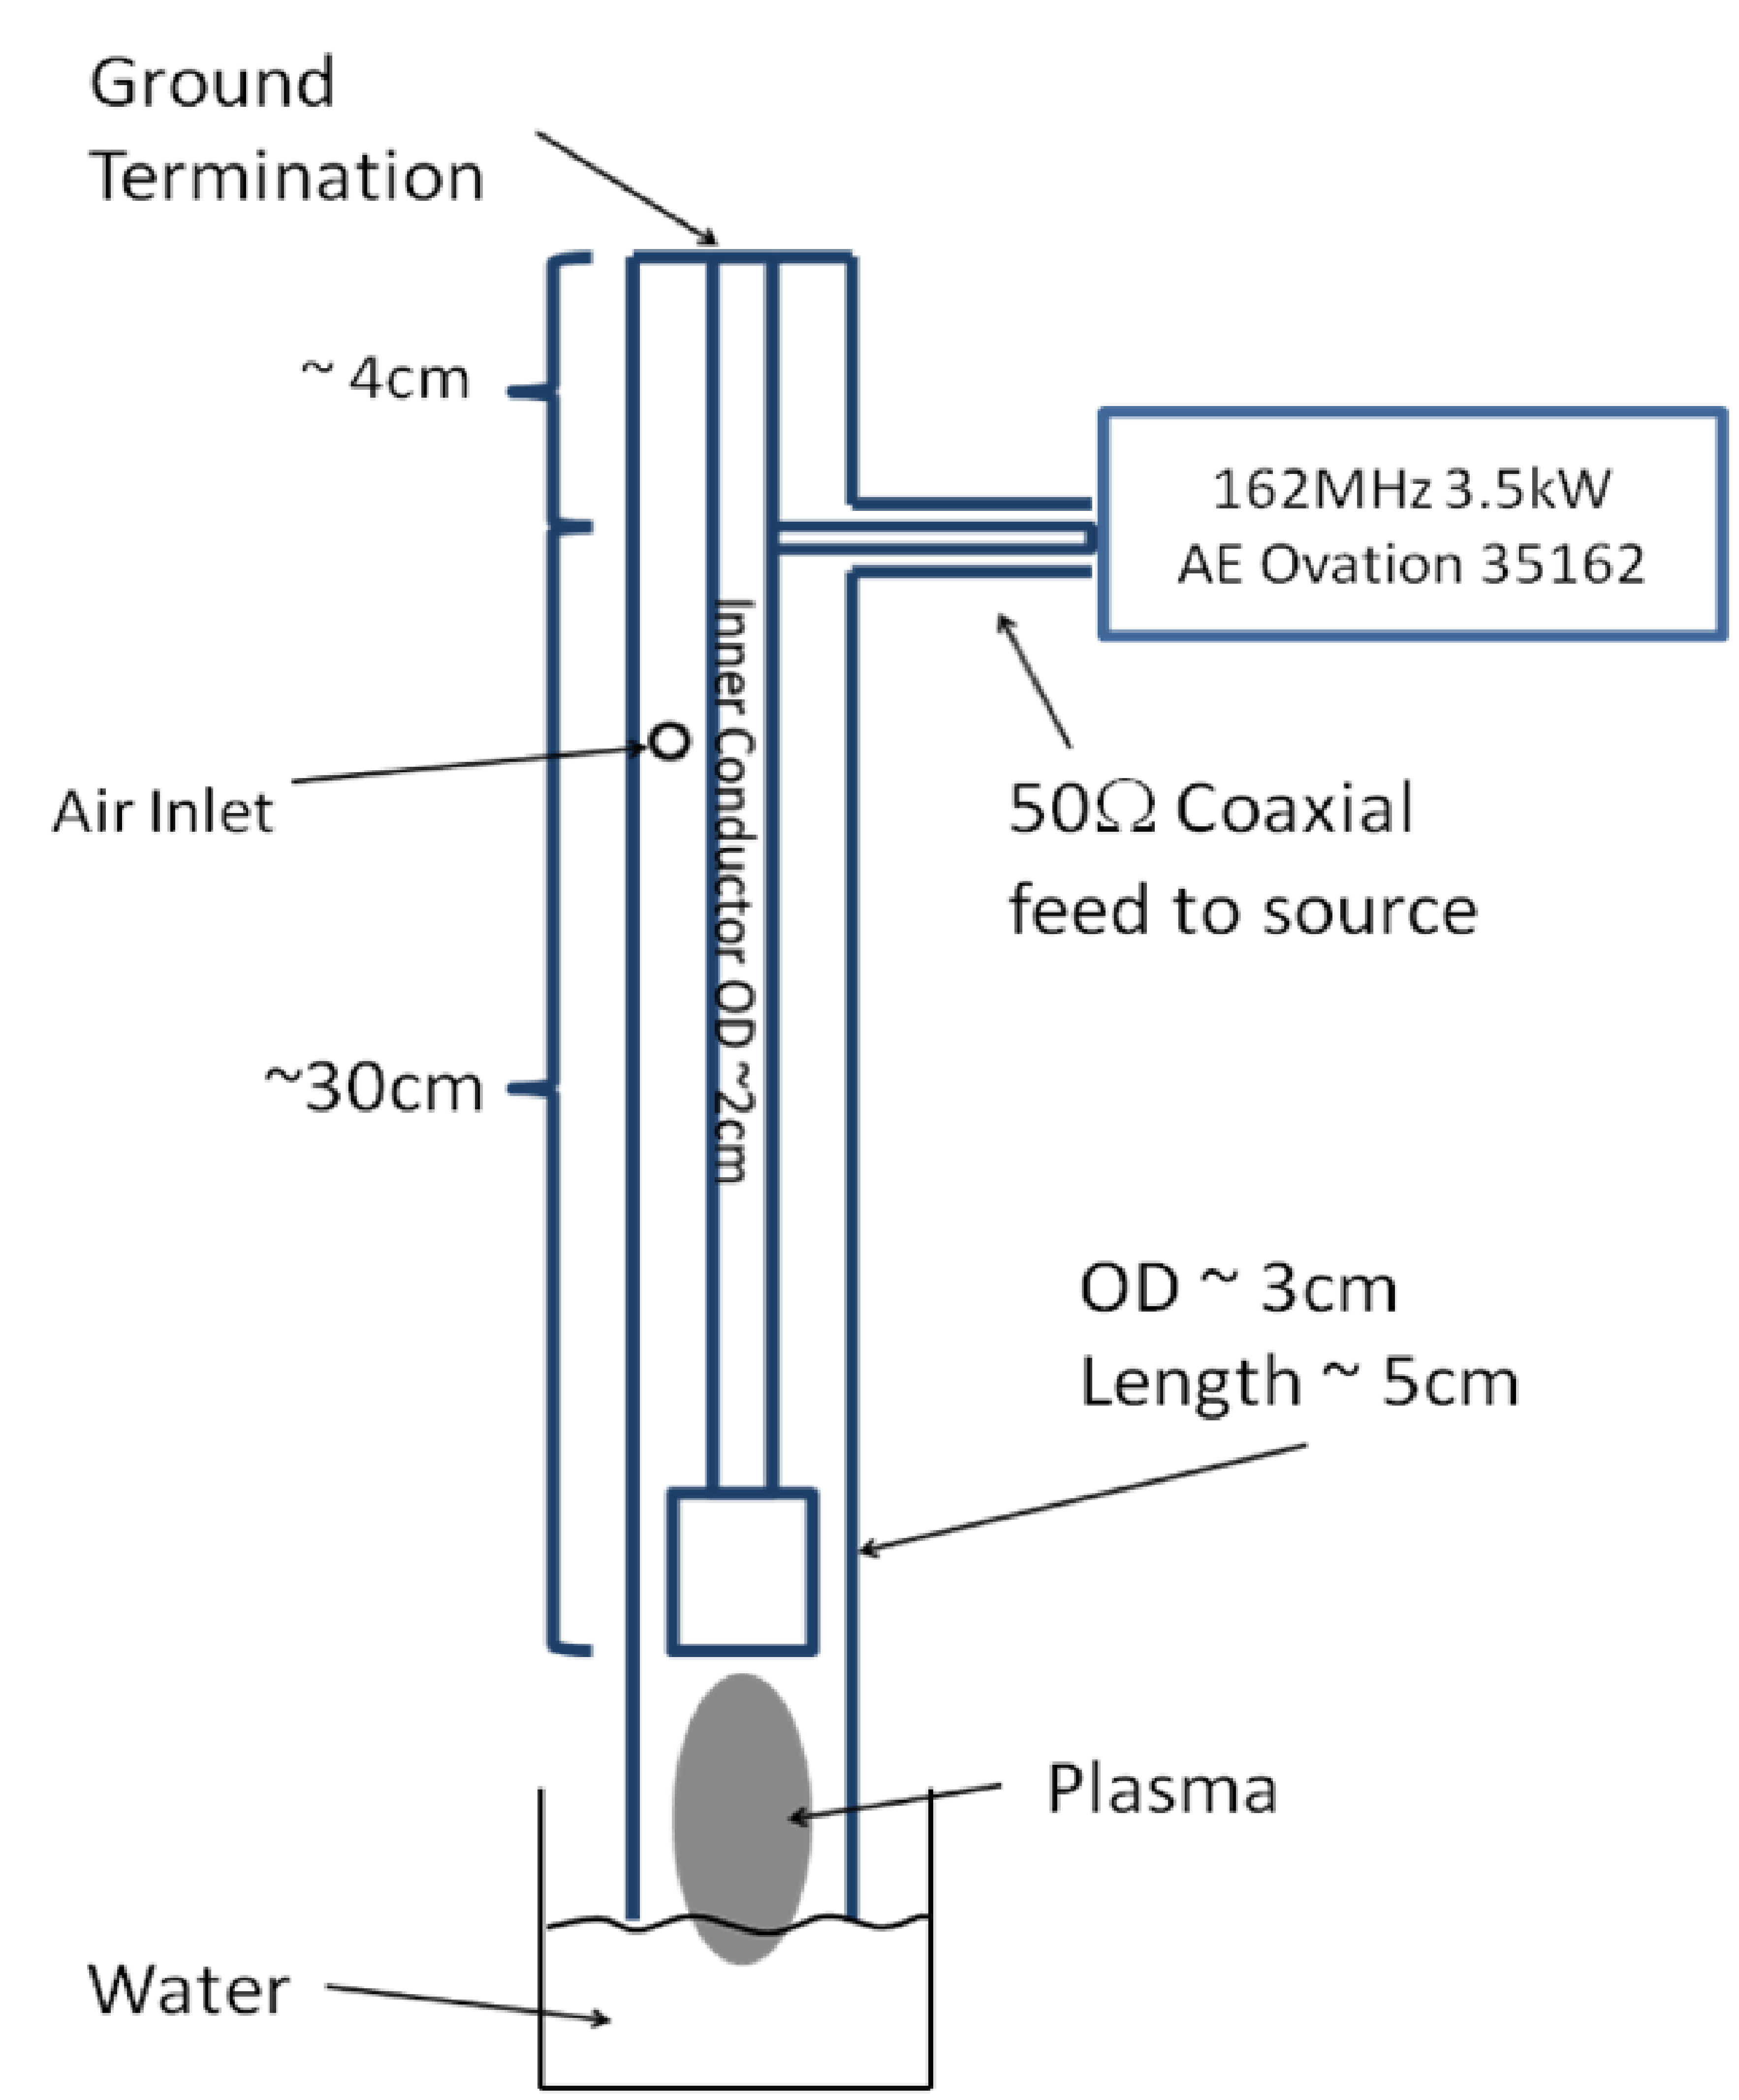
\includegraphics[width=0.9\textwidth]{Figure1_word.pdf}
  \caption{Schematic of the atmospheric plasma source and batch water treatment set-up}
  \label{fig:batch_scheme}
\end{figure}

\section{Spray-through Design}
\label{sec:spray}

One way thought to increase plasma-water interaction is to directly introduce water droplets into the active plasma region. We hypothesize that there are two good reasons for doing this. Firstly, it is reasoned that water droplets passing through the core of the plasma as opposed to the edge or afterglow are exposed to greater densities of electrons, ions, and reactive radical species. Secondly, by breaking the water volume into droplets, the surface-to-volume ratio is increased, increasing the rate of mass transfer of plasma species into the aqueous phase. Two different configurations are used to explore these concepts; they are outlined in the following subsections.

\subsection{Spray Bottle}
\label{sec:spray_bottle}

The easiest way to achieve a droplet configuration is to take the batch set-up (see \cref{fig:batch_scheme}) and remove the beaker of water under the coaxial plasma source. Then after turning the plasma on, a greenhouse sprayer is used to pass droplets radially through the plasma; a beaker is used to catch the droplets after passage through the plasma. A summary of the configuration is shown in \cref{fig:spray_scheme}.

\begin{figure}[htbp]
  \centering
  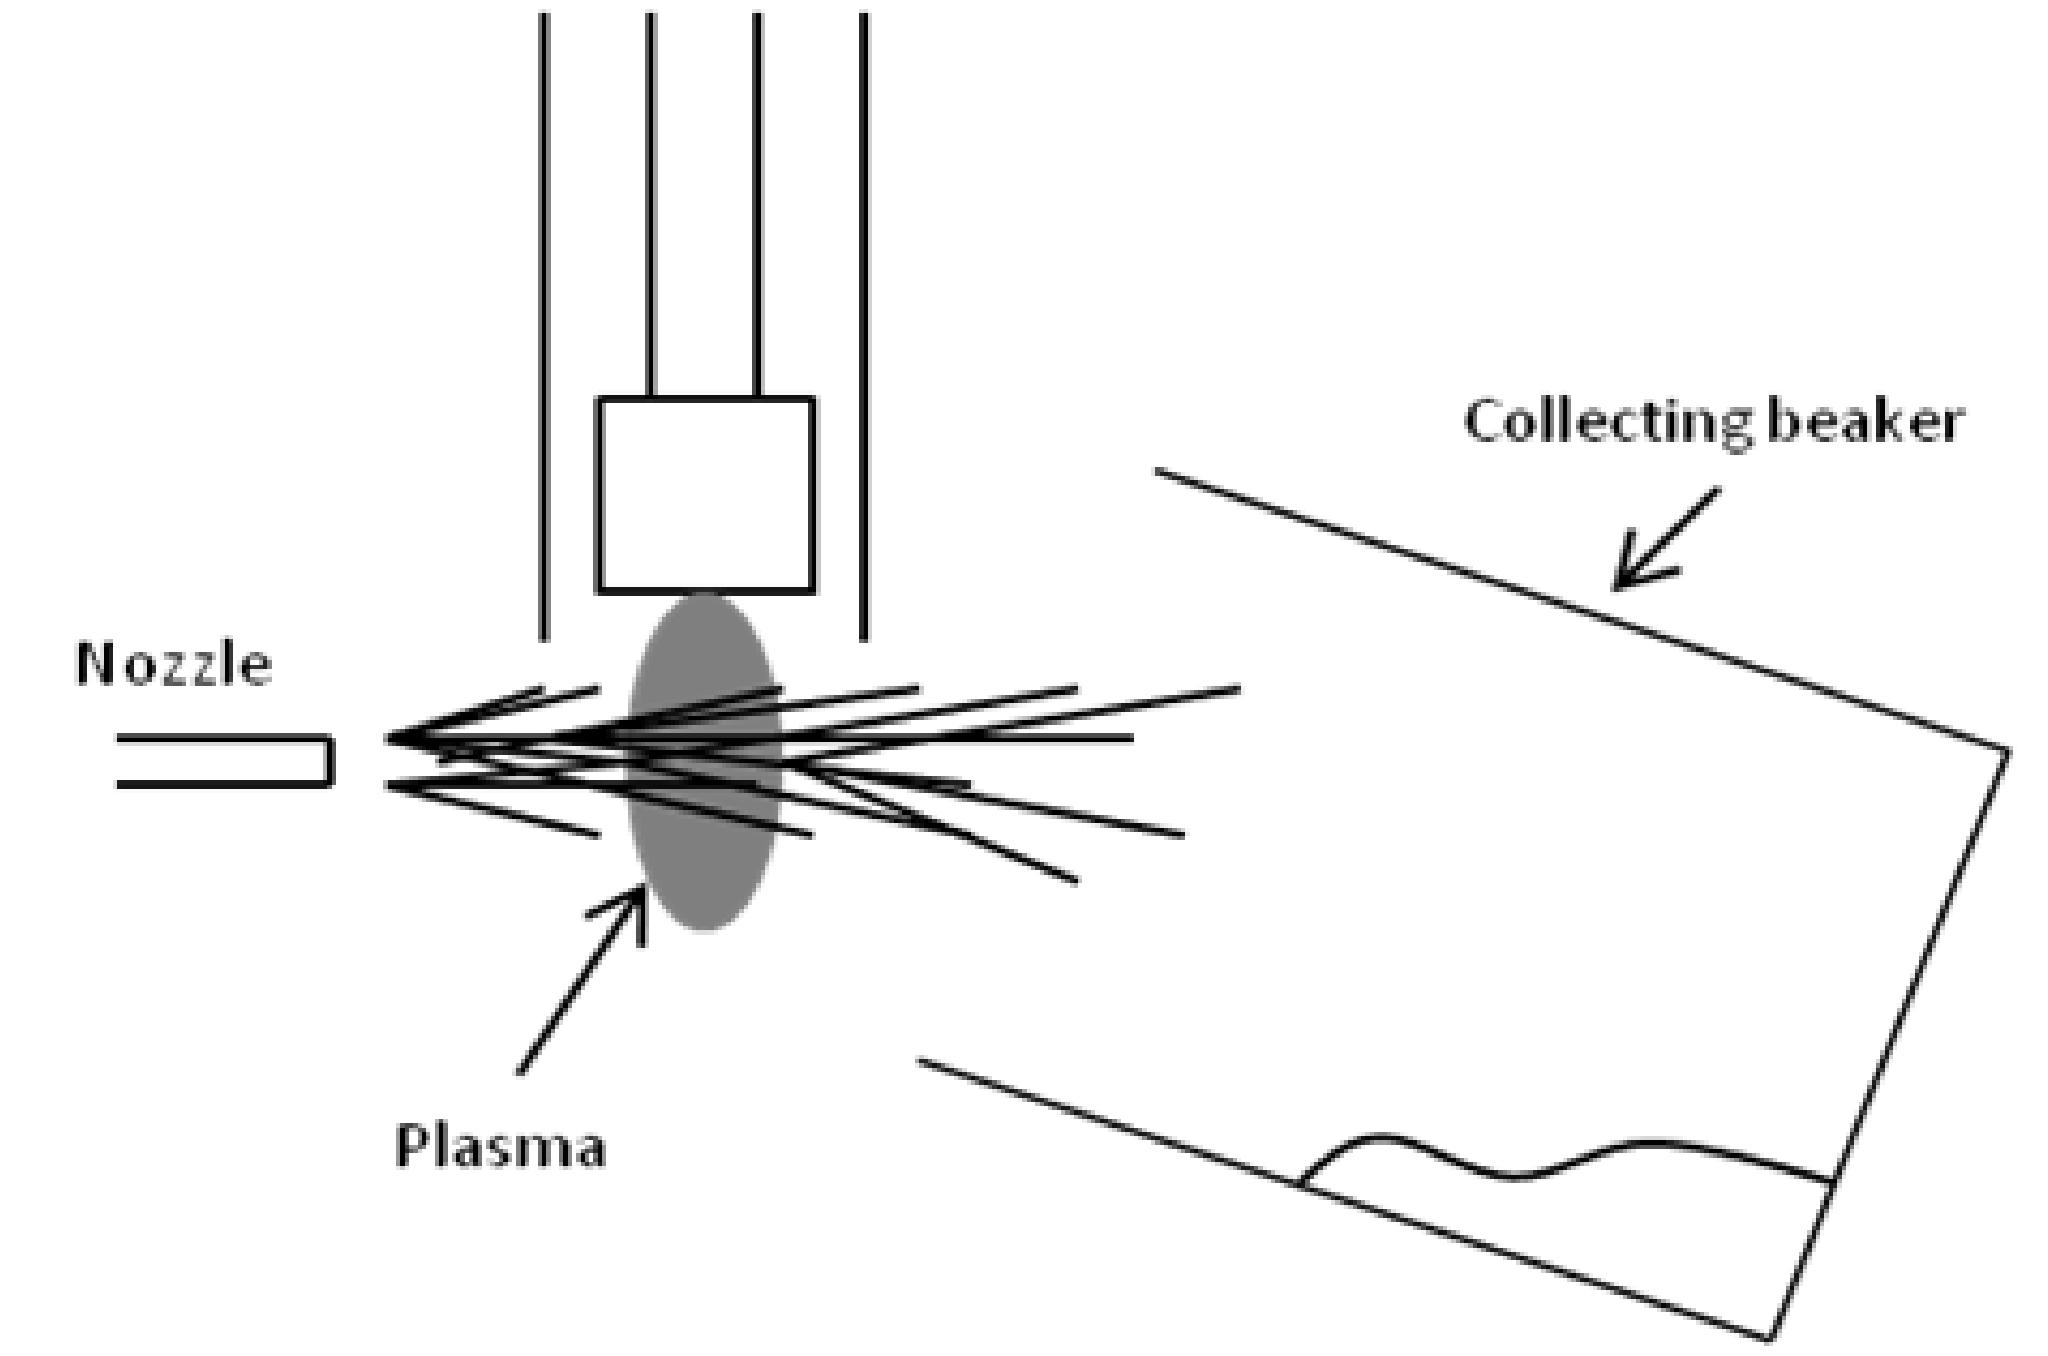
\includegraphics[width=0.9\textwidth]{Figure6_word.jpg}
  \caption{Set-up for introducing water directly into the active plasma region.  A greenhouse sprayer injects water from the side of the plasma source; water is collected in a beaker on the other side}
  \label{fig:spray_scheme}
\end{figure}

A comparison of batch and greenhouse sprayer configurations for generation of nitrate in solution per unit energy is shown in \cref{fig:nitro_compare_power_design}. It is found that in general the greenhouse sprayer configuration performs more favorably than the batch treatment design. This is especially clear at higher powers. Moreover, the performance of the greenhouse sprayer configuration appears to improve with increasing power delivered to the plasma. However, increasing plasma power also has some negative effects. One is an increased rate of erosion of the powered electrode. A second negative consequence is increased reflected power back to the generator during plasma instabilitiesarising from the water droplets. Both of these effects decrease the lifetime of the design; decreasing the lifetime of the generator is particularly undesirable because of its cost.

\begin{figure}[htbp]
  \centering
  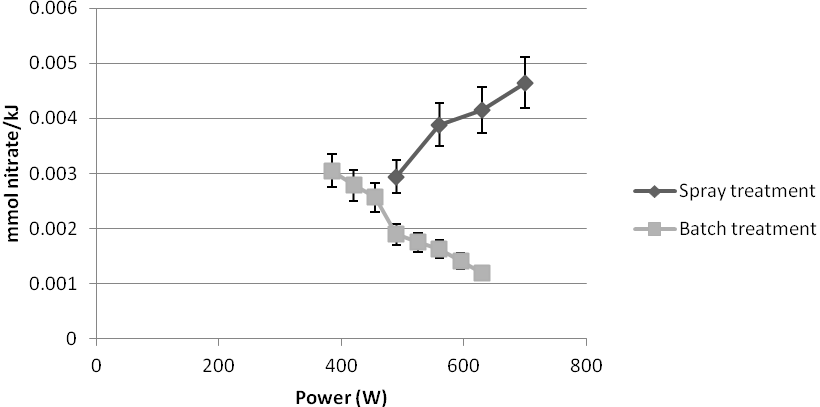
\includegraphics{Figure22_word.png}
  \caption{Comparison between batch and spray treatment methods using mmol of nitrate generated per kJ of electrical energy as the figure of merit.  For lower powers batch treatment is more energetically efficient for nitrate generation.  For higher powers, spray treatment is more efficient.}
  \label{fig:nitro_compare_power_design}
\end{figure}

What ultimately curtails further investigation of the spray-through design is the instability of the plasma. The sprayer must be placed such that droplets do not touch the surface of the powered electrode or else the plasma is immediately extinguished. Moreoever, even if the sprayer is properly placed and the electrode is not wetted, the plasma actively trys to avoid the droplet stream. This may occur for several reasons. Firstly, a much higher electric field must be applied to a dense liquid as opposed to a gas to create or sustain a discharge. Secondly, highly oxidative species like OH and OH$_2$ originating from the liquid phase can scavenge electrons. Typically even in the most optimized sprayer set-up, the plasma extinguishes after a few tens of seconds. Compare this with the batch set-up in which water can be treated continuously for multiple hours.

\subsection{Built-in Nozzle}

\begin{figure}[htbp]
  \centering
  \includegraphics{nozzle_diagram.png}
  \caption{Schematic of the nozzle electrode spray-through configuration}
  \label{fig:nozzle}
\end{figure}

\Cref{fig:nozzle} shows a schematic of the nozzle electrode experimental design. In terms of plasma-liquid contact, the concept is very similar to \cref{fig:spray_scheme} except the droplets are introduced vertically through the VHF source's inner conductor. Unfortunately, the nozzle electrode design suffers from the same pitfall as the greenhouse sprayer design. During operation, the plasma actively avoids the water droplets, moving with the cyclonic flow of the gas feed around the outside of the droplet stream. It is speculated that the droplet stream may form a partial Faraday cage inhibiting the discharge. Additionally, electronegative species like OH and OH$_2$ originating from the liquid phase may scavenge electrons in a manner analogous to the spray-through configuration of \cref{sec:spray_bottle}. On top of plasma instability originating from liquid interactions, the surface non-uniformity introduced by the nozzle on the electrode leads to faster surface erosion.

\section{Base electrode designs}
\label{sec:electrodes}

As mentioned in \cref{sec:spray_bottle}, plasma erosion of the source's powered electrode can occur, especially at higher powers. Evidence of this erosion can be seen both with the naked eye and in the optical emission spectrum of the discharge. \Cref{fig:OES_alum_damage} shows the presence of an atomic aluminum line at 395 nm and several AlO bands between 425 and 575 nm. Visually, this emission manifests itself as an intense bright blue. \Cref{fig:alum_damage_full} shows plasma color during normal operation, plasma color during aluminum damage, and the resulting appearance of the electrode after significant erosion.

\begin{figure}[htbp]
  \centering
  \includegraphics{damaged_aluminum_OES_spectrum.png}
  \caption{OES spectrum of plasma damaged aluminum electrode}
  \label{fig:OES_alum_damage}
\end{figure}

\begin{figure}[htbp]
  \centering
  \begin{subfigure}{.3\textwidth}
    \centering
    \includegraphics[width=\textwidth]{happy_plasma.jpg}
    \caption{Normal plasma color}
  \end{subfigure}
  \begin{subfigure}{.3\textwidth}
    \centering
    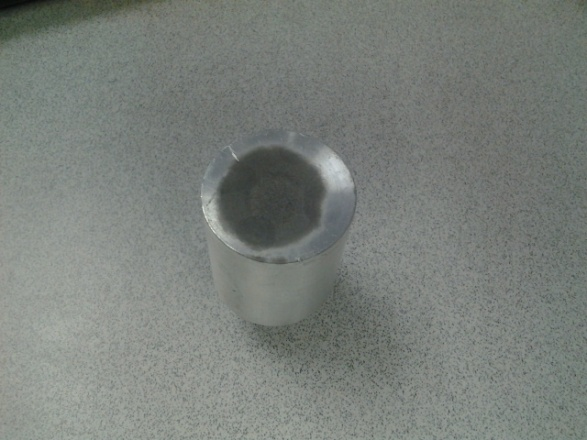
\includegraphics[width=\textwidth]{full_size_alum_electrode_damage.jpg}
    \caption{Image of aluminum electrode after plasma erosion}
  \end{subfigure}
  \begin{subfigure}{.3\textwidth}
    \centering
    \includegraphics[width=\textwidth]{argon_plasma_treating_dioxane.png}
    \caption{Plasma color during aluminum pitting}
  \end{subfigure}
  \caption{Normal vs. abnormal plasma glows}
  \label{fig:alum_damage_full}
\end{figure}

The plasma damage to the electrode can be investigated more closely using Secondary Electron Microscopy (SEM) and Energy Dispersive X-ray Spectroscopy (EDS). Even with a 1mm zoom (\cref{fig:alum_damage_1mm}), the growth of a damage layer is evident. Taking an EDS measurement of the clean aluminum yields the spectrum shown in \cref{fig:EDS_clean_alum}. Unsurprisingly, the spectrum shows almost pure aluminum with a trace of magnesium. An EDS scan of the damaged aluminum portion, however, reveals the growth of substantial carbon and oxygen peaks (\cref{fig:EDS_damaged_alum}). The oxidation is unsurprising considering the flow gas is often compressed air and the ambient environment is also air (also consistent with the OES spectrum (\cref{fig:OES_alum_damage})). The carbon could be coming from oils/hydrocarbons present in the compressed air feed.

\begin{figure}[htbp]
  \centering
  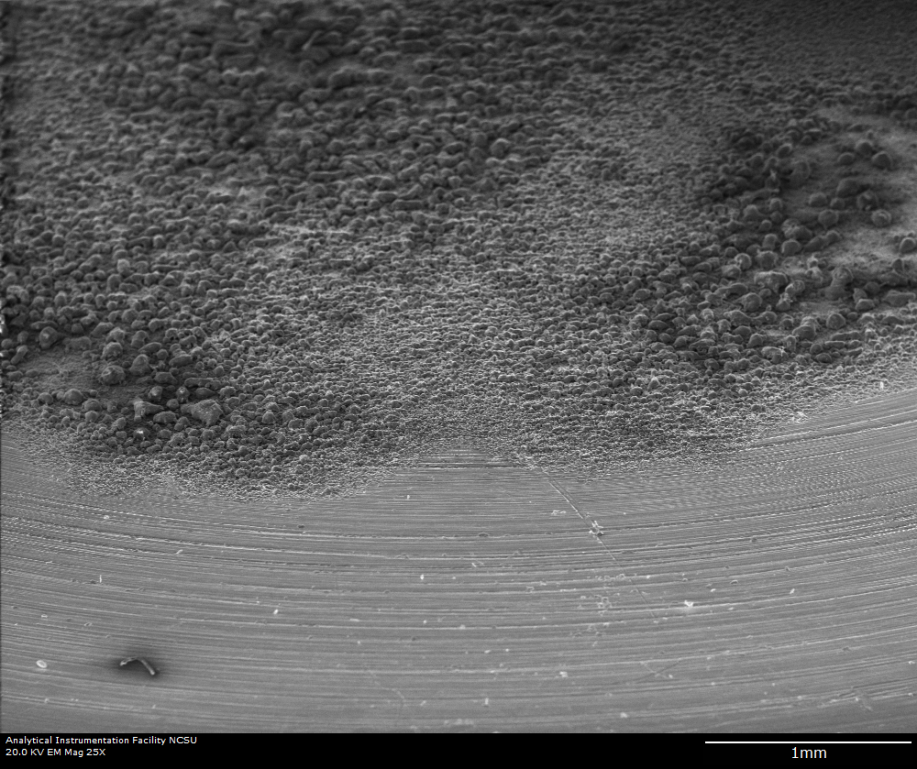
\includegraphics{1mm_zoom_tilt_alum_electrode_damage.png}
  \caption{SEM image of aluminum electrode after plasma erosion. 1mm zoom. 45 degree tilt.}
  \label{fig:alum_damage_1mm}
\end{figure}

\begin{figure}[htbp]
  \centering
  \includegraphics[width=0.9\textwidth, height=0.9\textheight, keepaspectratio]{clean_alum_eds.png}
  \caption{Energy dispersive X-ray spec (EDS) for clean aluminum electrode}
  \label{fig:EDS_clean_alum}
\end{figure}

\begin{figure}[htbp]
  \centering
  \includegraphics[width=0.9\textwidth, height=0.9\textheight, keepaspectratio]{damaged_alum_eds.png}
  \caption{Energy dispersive X-ray spec (EDS) for plasma eroded aluminum electrode}
  \label{fig:EDS_damaged_alum}
\end{figure}

In an attempt to prolong the lifetime of the powered electrode, metals other than aluminum are considered. A relatively inexpensive choice is brass. Overall, brass performs much better than aluminum. Between 300-700 W, there is no plasma-metal interactions observed with OES or presence of pitting when the plasma is turned off. Typically aluminum begins to erode around 560 W. When the brass electrode is run between 700-1000 W, plasma-metal interactions are evinced by a plasma color change as well as an increase in the intensity of the emitted light. A comparison of the plasma OES with and without metal interactions is shown in \cref{fig:OES_brass_damage}. The 560 W spectrum shows a more or less normal air plasma spectrum: NO bands between 230 and 290 nm (along with their 2x peaks around 500nm) and an OH band around 310 nm. However, the 945 W spectrum is dominated by sharp copper and zinc atomic lines. Despite the presence of copper and zinc in the discharge emission, no visual damage appears on the electrode surface when operated between 700 and 1000 W. However, if the power is raised too much over 1000 W, surface pitting and scarring analagous to the damage on the aluminum electrode are observed (see \cref{fig:brass_damage_full}).

\begin{figure}[htbp]
  \centering
  \includegraphics[width=0.9\textwidth]{damaged_brass.jpg}
  \caption{Image of brass electrode after plasma erosion}
  \label{fig:brass_damage_full}
\end{figure}

\begin{figure}[htbp]
  \centering
  \includegraphics{damaged_brass_OES_spectrum.png}
  \caption{Top OES spectrum shows plasma emissions during normal operation with the brass electrode. The bottom spectrum shows emissions that occur during brass damage}
  \label{fig:OES_brass_damage}
\end{figure}

\section{Water Electrodes}
\label{sec:water_electrodes}

An ideal plasma-liquid geometry has to provide both maximum interfacial contact between reactive plasma species and the liquid phase as well as system components that are resistent to plasma corrosion. Unfortunately, none of our previous configurations realize this goal. However, by utilizing the unique nature of the VHF source and recognizing that the entire coaxial structure is DC grounded, we can do something rather novel. We can apply a liquid layer to the surface of the powered electrode without worry of causing a short circuit. With this configuration, shown in \cref{fig:water_electrode_scheme}, the treated water is exposed to the most reactive part of the plasma. Both ion and electron fluxes to the water surface are anticipated to be much higher than in the batch configuration. Additionally, powered plasma-facing solid surfaces are completely eliminated from the geometry. The liquid surface is forever renewable and does not erode. This reduces system cost as well as experimental down-time.

\begin{figure}[htbp]
  \centering
  \includegraphics[width=0.9\textwidth]{water_electrode_geometry.png}
  \caption{Representative experimental set-up for using a ``water'' electrode}
  \label{fig:water_electrode_scheme}
\end{figure}

The actual design of the water electrode can be seen in \cref{fig:water_electrodes_image}. The electrode of most utility, the ``pure'' water electrode, is shown on the right. The pure water electrode has no powered metal surfaces facing the plasma; the powered plasma-facing surface is 100\% water. If some plasma-metal contact is desired, for instance if the contact favorably modifies some plasma or liquid application variable, then the ``annular'' electrode shown on the left can be used.

\begin{figure}[htbp]
  \centering
  \includegraphics[width=0.9\textwidth]{water_and_annular_electrodes.jpg}
  \caption{Image of the two versions of ``water'' electrodes. The ``annular'' version still allows a small metallic area of plasma contact. In the ``pure'' version, the plasma has no metallic content with the powered electrode. The powered surface is entirely composed of water.}
  \label{fig:water_electrodes_image}
\end{figure}

\subsection{Circuit Analysis}
\label{sec:circuit}

In order to better understand the coupling of the RF power to the plasma-liquid system, it is useful to construct a circuit model. The first question the circuit model should answer is whether conduction current coming from the inner conductor propagates along the water electrode surface or the underlying aluminum. This is done by comparing the relative resistances presented by the water and aluminum surfaces, treating both as conductors. The resistance is calculated using the relationship:

\begin{equation}
  R = \frac{L\rho}{A}
  \label{eq:skin_R}
\end{equation}

where $R$ is the resistance, $L$ is the length of the conducting surface, $\rho$ is the resistivity of the medium, and $A$ is the cross-sectional area through which the conduction current can flow. For current propagation across the top face of the cylindrical electrode, we approximate $L$ by the radius $r$ of the electrode, and $A$ by the product of the skin depth $\delta$ and the radius $r$. The skin depth $\delta$ is calculated using:

\begin{equation}
  \delta = \sqrt{\frac{2\rho}{\omega\mu_B}}
  \label{eq:skin_depth}
\end{equation}

where $\omega$ is the driving frequency in radians/s and $\mu_B$ is the material permeability, set equal to $\mu_0=4\pi\times10^{-7}$. For aluminum, $\rho$ is set equal to its literature value at 20$^{circ}$ Celsius, $2.82\times10^{-8}\Omega m$. A typical tap water conductivity of 50 mS/m is used to calculate the resistivity of water, $\rho = \frac{1}{\sigma}$. The corresponding skin depth for water at 162 MHz is .18 m, which is significantly larger than the milimeter depth of the water layer. As a consequence, $A$ for \cref{eq:skin_R} is calculated with $\delta$ = 1 mm. With these definitions,tThe resistance of the water surface to conduction current is calculated to be 20 thousand $\Omega$ at 162 MHz. The skin depth of aluminum at 162 MHz is 6 $\mu$m. The corresponding resistance to conduction current is 4 m$\Omega$ at 162 MHz. One can ask whether plasma modification of the water surface might substantially decrease the water resistance; however, because the mobility of electrons in water is so much lower than their gaseous mobility, the effect of the plasma is nowhere near enough to overcome the seven order of magnitude difference in resistance between water and aluminum. This analysis suggests that all of the conduction current coming from the feed line propagates along the underlying aluminum electrode as opposed to the water surface. A frequency analysis shown in \cref{fig:surf_propag} demonstrates that conduction current will likely flow through the underlying aluminum regardless of the device operating frequency.

\begin{figure}[htbp]
  \centering
  \includegraphics[width=0.9\textwidth]{alum_vs_water_propagation.eps}
  \caption{Resistance to flow of conduction current for aluminum and water for a range of frequencies. Vertical, black, dotted line indicates the 162 MHz operating frequency of the NCSU source. Aluminum is orders of magnitude less resistive for all frequencies considered; consequently the current propagating along the feed line is likely to prefer the underlying aluminum electrode over the water surface.}
   \label{fig:surf_propag}
\end{figure}

The demonstration that conduction current likely does not propagate along the water \textit{surface} means that current, most likely in the form of displacement current, must pass through the water \textit{volume}. The question then becomes: what is the relative split in dissipated power between the water and plasma? Where is the potential drop occuring? These are answered by treating the water volume and plasma as lossy dielectrics. We define the medium dielectric constant by:

\begin{equation}
  \epsilon = \epsilon_r\epsilon_0\left(1 - \frac{\omega_c^2}{\omega\left(\omega - \nu j\right)}\right)
  \label{eq:epsilon}
\end{equation}

where $\epsilon_r$ is the relative dielectric constant, $\epsilon_0$ is the permittivity of free space, $\omega_c$ is the characteristic frequency coming from oscillatios of free charges in the medium, $\omega$ is again the driving frequency, $\nu$ is the rate of collisions of charges with background molecules, and j is the imaginary number $\sqrt{-1}$. For the plasma, $\epsilon_r=1$; for the water, $\epsilon_r=80$. Because the free electrons are much lighter than their corresponding ions, $\omega_c$ in the plasma is essentially equal to the plasma electron frequency $\omega_{pe}$. In the water, $\omega_c$ is calculated assuming sodium and chloride charge carriers. $\omega_c$ in both plasma and water is calculated using the equation:

\begin{equation}
  \omega_c = \sqrt{\frac{e^2n_0}{\epsilon_0 m}}
  \label{eq:omega_c}
\end{equation}

where $e$ is the Coulombic charge, $n_0$ is the number density, and $m$ is the particle mass. For the plasma, $\nu$ is calculated using:

\begin{equation}
  \nu = n_g\sqrt{\frac{\pi \alpha e^2}{m_e\epsilon_0}}
  \label{eq:nu_plasma}
\end{equation}

where $n_g$ is the background gas density and $\alpha$ is the polarizability equal to $2.1\times10^{-29}m^3$ for air. For the water, $\nu$ is determined via

\begin{equation}
  \nu = \frac{e}{\mu m}
  \label{eq:nu_water}
\end{equation}

where $\mu$ is the mobility calculated with Einstein's relation

\begin{equation}
  \mu = \frac{D e}{k_b T}
  \label{eq:einstein}
\end{equation}

where D is the diffusivity of sodium and chloride ions, equal to $2\times10^{-9}m^2s^{-1}$ \cite{morrow2006time}, $k_b$ is Boltzmann's constant, and T is the temperature of the water (assumed equal to 300 K). Once the medium dielectric constant $\epsilon$ is calculated, the medium admittance is computed using the approximation of a parallel plate capacitor:

\begin{equation}
  Y = \frac{\omega \epsilon A j}{d}
  \label{eq:admittance}
\end{equation}

Finally, the impedance $Z$ is computed using the simple relation, $Z = \frac{1}{Y}$. For a lossy dielectric, the impedance $Z$ is complex, e.g. $Z = R + Xj$ with R the resistance and X the reactance. \Cref{fig:resist_compare} compares the plasma and water resistance over a wide range of frequencies. Over the entire range of frequencies presented the water resistance is < 1\% of the plasma resistance. At the operating frequency of the VHF source, the water resistance is close to six orders of magnitude less than the plasma resistance, suggesting that virtually all of the RF power is dissipated in the plasma.

\begin{figure}[htbp]
  \centering
  \includegraphics[width=0.9\textwidth]{Plasma_vs_water_resistance.eps}
  \caption{Comparison of plasma and water resistances over a range of operating frequencies. Over the whole domain, the water resistance is < 1\% the plasma resistance. At 162 MHz they differ by six orders of magnitude, suggesting that all of the RF power is dissipated in the plasma as opposed to the water.}
  \label{fig:resist_compare}
\end{figure}

\Cref{fig:react_compare} compares the magnitude of the plasma and water reactance as a function of frequency. For both mediums, the reactance is negative for all frequencies, consistent with capacitive behavior. (Lower gas pressures lead to more inductive behavior.) For frequencies < 1 MHz, the plasma and water reactance are roughly equivalent. Beyond 1 MHz, the magnitude of the water reactance decreases while the magnitude of the plasma reactance continues to increase until roughly 80 MHz beyond which it begins to decline. \Cref{fig:imped_mag} compares the magnitude of the impedance ($|Z| = \sqrt{R^2 + X^2}$) for plasma and water for a range of frequencies. The impedance magnitude for water is determined primarily by its resistive component below 1 MHz and by its reactive component above 1 MHz. The behavior for the plasma is similar except the transition occurs around 30 MHz. The result is that the plasma impedance magnitude is always a couple of magnitudes larger than the water impedance magnitude for all frequencies, ensuring that the majority of the potential drop always occurs across the plasma as opposed to the water.

\begin{figure}[htbp]
  \centering
  \includegraphics[width=0.9\textwidth]{Plasma_vs_water_reactance.eps}
  \caption{Comparison of plasma and water reactance magnitude for a range of frequencies. Magnitudes are roughly equivalent up to 1 MHz, where water reactance magnitude begins to decline. Plasma knee occurs around 80 MHz.}
  \label{fig:react_compare}
\end{figure}

\begin{figure}[htbp]
  \centering
  \includegraphics[width=0.9\textwidth]{Plasma_vs_water_impedance_mag.eps}
  \caption{Impedance magnitudes for plasma and water as a function of frequency. Plasma impedance magnitude is significantly larger over the whole frequency domain.}
  \label{fig:imped_mag}
\end{figure}

\subsection{Optical Emission}
\label{sec:OES}

\Cref{fig:annular_vs_water_oes} compares typical OES spectra obtained for annular and pure water electrodes running at 700 W. Evidence of plasma-metal contact with the annular electrode is evident in the presence of aluminum atomic lines and AlO molecular bands. Additionally, there is a sodium line from sputtering of the tap water. The pure water electrode spectrum is much less intense and consists only of OH bands.

\begin{figure}[htbp]
  \centering
  \includegraphics{annular_vs_water_electrode_oes.png}
  \caption{Comparison of OES spectra for annular and pure water electrodes}
  \label{fig:annular_vs_water_oes}
\end{figure}

\Cref{fig:pow_sweep_water} shows the effect of increasing power on the optical emission spectrum with the pure water electrode. Because the plasma is in immediate contact with the water surface and not any solid surfaces, the device can be operated at much higher powers. Whereas with a metal electrode the source cannot be run at powers much greater than 700 W without significant damage to the electrode, the pure water electrode can be run up to 1155 W. The only reason that the device cannot be operated at even higher powers is because of the increased difficulty in matching impedances using the main and stub lines; reflected power becomes high enough to potentially damage the generator.

Up above 1000 W, aluminum atomic lines and AlO bands become apparent (\cref{fig:pow_sweep_water}). The presence of the aluminum associated emissions is interesting because the metal is removed from the gaseous discharge region by the few milimeter thick water layer; this probably explains why the intensities are significantly below that of discharges with direct plasma-metal contact (see \cref{fig:annular_vs_water_oes}). However, the existence of any aluminum lines at all implies that the discharge is penetrating the aqueous phase to reach the metal. This is perhaps indirect evidence of high charged particle fluxes to the water electrode surface, suggesting that the pure water electrode design is a good one for maximizing interactions between the plasma and aqueous phases.

\begin{figure}[htbp]
  \centering
  \includegraphics{water_electrode_power_sweep_oes.png}
  \caption{OES spectra showing power sweep with pure water electrode. Relatively small aluminum peaks grow in at very high powers. Cause of aluminum peak deformations unknown, but speculation is that it could be signal attenuation by the water layer}
  \label{fig:pow_sweep_water}
\end{figure}

% Note that there is a lot of OH rotational measurement as well as nitrite and nitrate concentration measurements for the water electrodes that are in my ICOPS 2014 presentation. I think the data looks like a bunch of garbage with no clear trends so I'm omitting it for now. However, if I need more material, I can perhaps come back to it.

\subsection{Absorption Work}
\label{sec:absorption}

Some idea of the magnitude of OH produced by the water electrode geometry can be gained by performing absorption spectroscopy. A picture of the experimental set-up is shown in \cref{fig:expt_abs}. The diameter of the plasma column is approximately 2 cm. We pass a broadbeam light source through slits cut in the outer conductor of the VHF shource. Mirrors on each slit side can be used to route the light beam through the plasma column for a total of up to 4 passes and a path-length up to 8 cm. After passing through the plasma, the beam enters an optical fiber connected to a high resolution spectrometer. The spectrum of the broadband light source in the absence of plasma is presented as series ``no-plasma'' in \cref{fig:raw_abs}. When the plasma is turned on, there is significant attenuation of the broadband signal in the region of the OH X-A electronic transition with just a single pass through the plasma as shown in \cref{fig:raw_abs}. The y-axis data for \cref{fig:net_abs} is calculated using:

\begin{equation}
  1 - \frac{I-I_p}{I_0}
  \label{eq:absorp}
\end{equation}

where $I$ is the spectrum taken with both the broadband light source and plasma, $I_p$ is the spectrum of plasma only, and $I_0$ is the spectrum of just the broadband light source. The fingerprint of the OH X-A transition is evident.

\begin{figure}[htbp]
  \centering
  \includegraphics[width=\textwidth]{abs_setup.png}
  \caption{Expermental set-up for absorption spectroscopy with the water electrode.}
  \label{fig:expt_abs}
\end{figure}

\begin{figure}[htbp]
  \centering
  \includegraphics[width=\textwidth]{raw_absorption_spec.png}
  \caption{Raw optical spectra in the OH wavelength region for different plasma powers and a path length of 2 cm (single pass). The series ``No plasma'' shows the light intensity of just the broadband light source. The other series clearly show the absorption of light by gaseous OH radicals. Highlighted region shows the area of integration for later calculation of OH densities}
  \label{fig:raw_abs}
\end{figure}

\begin{figure}[htbp]
  \centering
  \includegraphics[width=\textwidth]{net_absorption_spec.png}
  \caption{Net results obtained by subtracting plasma absorption spectra from broadband light source spectrum and normalizing. Obvious OH X-A transition fingerprint. Highlighted region shows the area of integration for later calculation of OH densities}
  \label{fig:net_abs}
\end{figure}

We can approximately calculate the density of ground-state OH in the plasma using Beer-Lambert's law:

\begin{equation}
  \frac{I-I_p}{I_0} = exp\left(-\sigma(\lambda) L N\right)
  \label{eq:beer-lambert}
\end{equation}

where $\sigma$ here is the cross section in units of area for absorption of light of wavelength $\lambda$, $L$ is the path length for absorption, and $N$ is the density of the absorbing species, OH in this case. Because the OH(X-A) transition is spread over a variety of vibrational and rotational states, one can choose a wavelength range to integrate over. As indicated by the highlight in \cref{fig:raw_abs,fig:net_abs}, the wavelengths spanning the P branch, roughly 309-309.5 nm, are chosen for integration. When performing the integration,

\begin{equation}
  \int_{309}^{309.5} \left(1 - \frac{I-I_p}{I_0}\right)d\lambda = \int_{309}^{309.5}\left(1 - exp\left(-\sigma(\lambda) L N\right)\right)d\lambda
  \label{eq:int_unsimplified}
\end{equation}

the integrand on the RHS can be simplified because the argument of the exponential is small, allowing the approximation $exp(-x)\approx 1 - x$. After performing this substitution, the concentration of OH can be calculated using:

\begin{equation}
  N = \frac{\int_{309}^{309.5}\left(1 - frac{I-I_p}{I_0}\right)d\lambda}{L\int_{309}^{309.5}\sigma(\lambda)d\lambda}
  \label{eq:int_simp}
\end{equation}

\Cref{fig:OH_dist} shows the density of OH as a function of distance from the powered electrode for powers of 455, 560, and 665 W. OH densities are on the order of 10$^{15}$ cm$^{-3}$. The density decreases monotonically with increasing distance from the powered electrode.

\begin{figure}[htbp]
  \centering
  \includegraphics[width=\textwidth]{distance_vs_OH_density.png}
  \caption{OH density versus position from the powered electrode for a variety of powers}
  \label{fig:OH_dist}
\end{figure}

\Cref{fig:OH_pow} shows the OH density as a function of power at a distance of 8 cm from the powered electrode. From 455 to 700 W the OH density increases linearly from a minimum value of 2x10$^{14}$ cm$^{-3}$ to a maximum value of 1.2x10$^{15}$ cm$^{-3}$. These high OH densities could be valuable in applications requiring a high degree of oxidative stress, such as in various fields of plasma medicine and pollutant degradation. Concentrated OH could be a key player in the degradation of persistent chemicals like dioxane and PFOS, as described in \cref{sec:pollutant}.

\begin{figure}[htbp]
  \centering
  \includegraphics[width=\textwidth]{OH_dens_vs_power.png}
  \caption{OH density versus power 8 cm from the powered electrode. Clear increasing trend of OH density with power}
  \label{fig:OH_pow}
\end{figure}

\section{Exploring Aqueous Chemistry Generated by Plasma-Liquid Interactions}
\label{sec:aq_chem}

In addition to plasma characterization with OES and absorption spectroscopy, additional research has focused on optimizing and understanding generation of nitrates and nitrites in aqueous solution.  Several variables have been explored, including power supplied by the 162 MHz generator, flow rate of the feed gas, type of interface between the plasma and water phases, and the effect of aqueous impurities, particularly basic species. The majority of experiments were performed using the experimental set-up shown in \cref{fig:batch_scheme}.  However, the greenhouse sprayer scheme shown in \cref{fig:spray_scheme} was also employed.  The number of impurities and basic species in water were controlled in two manners.  The first was the choice between distilled and tap water, with the former containing negligible impurities and the latter containing impurities found in Raleigh's municipal water supply; these impurities are summarized in \cref{tab:tap_water}.  The most relevant item in \cref{tab:tap_water} is the alkalinity, which comes primarily from the carbonate system.  At a pH of 8.4, it is reasonable to assume that the tap water alkalinity is completely due to bicarbonate. \cite{benjamin2014water} Using this assumption, the concentration of bicarbonate in tap water is .50 mmol/L.  The concentration of bicarbonate can also be directly controlled by adding measured amounts of NaHCO$_3$.   NaHCO$_3$ can be added pre- or post-exposure depending on the experiment.  The motivation for adding basic species like NaHCO$_3$ to solution is that they are known to react with dissolved NO and NO$_2$ to form nitrite. \cite{greenwood1984chemistry} Thus basic species concentrations can be a control knob for adjusting the nitrogen chemistry in PAW.

\begin{table}[htpb]
  \begin{center}
    \begin{tabular}{|c |c |}
      \hline
      pH & 8.4 \\\hline
      Free CO$_2$ & .23 \\\hline
      Total alkalinity (mg/L as CaCO$_3$) & 24.8 \\\hline
      Total hardness (mg/L as CaCO$_3$) & 24.4 \\\hline
      Total dissolved solids (mg/L) & 150 \\\hline
      Specific conductivity ($\mu$S/cm) & 225 \\\hline
      Iron (mg/L) & .01 \\\hline
      Manganese (mg/L) & .02 \\\hline
      Fluoride (mg/L) & .78 \\\hline
      Chloride (mg/L) & 13.3 \\\hline
      Silica (mg/L) & 8.12 \\\hline
      Silt density index (SDI) & 5.00 \\
      \hline
    \end{tabular}
  \end{center}
  \caption{Impurities in Raleigh tap water}
  \label{tab:tap_water}
\end{table}

At a gas flow rate of .14 m$^3$/min, an exposure time of 3 minutes, and a treatment volume of 150 mL distilled water, nitrate concentrations were determined for powers ranging from 385 to 630 W and are shown in \cref{fig:nitrogen_vs_energy}.  For a better comparison with spray treatment results shown in \cref{fig:nitrogen_vs_energy_spray}, the horizontal axis is defined in terms of the energy deposited in the plasma per mass of water exposed to the plasma.  The results indicate a general downward trend in nitrate concentration with respect to power and total energy deposition.   To decouple the effects of power and total energy deposition, a second experiment was conducted in which treatment times were varied with power in order to keep the total energy delivered to the plasma constant.  Consequently, whereas the exposure time was 3 minutes for a 420 W plasma, exposure time was only 2 minutes for a 630 W plasma for a constant plasma energy deposition of 75.6 kJ; for comparison with \cref{fig:nitrogen_vs_energy}, the energy deposited in the plasma per mass of exposed water was 504 kJ/kg.  Gas flow was again .14 m$^3$/min and water volumes were 150 mL.  Results from the second experiment are shown in \cref{fig:nitrogen_vs_power}.  Though the plasma energy deposition is constant, nitrate concentrations in both tap and distilled water samples decrease with increasing power, consistent with the trend in \cref{fig:nitrogen_vs_energy}.  Though no nitrite appears in distilled water samples, nitrite concentrations increase in tap water with increasing power.  The total nitrogen anion levels in tap and distilled water samples are within experimental error for powers between 420 and 560 W.

\begin{figure}[htbp]
  \centering
  \includegraphics{Figure17_word.png}
  \caption{Nitrate concentration in distilled water versus energy deposited in the plasma per mass of exposed water. No detectable amount of nitrite generated}
  \label{fig:nitrogen_vs_energy}
\end{figure}

\begin{figure}[htbp]
  \centering
  \includegraphics{Figure18_word.png}
  \caption{Nitrate and nitrite concentrations in tap water versus power.  Treatment times scaled such that for each power setting, total energy deposited in system is constant at 504 kJ/kg H2O}
  \label{fig:nitrogen_vs_power}
\end{figure}

Another variable explored was gas flow rate.  For an exposure of 3 minutes, a treatment volume of 150 mL distilled water, and a plasma power input of 420 W, nitrate concentrations were measured for flow rates of .08, .11, and .14 m$^3$/min and are recorded in \cref{fig:nitrogen_vs_flow}.  A factor of 4.9 improvement in nitrate concentration is observed between .08 and .14 m$^3$/min flow settings.  Again no detectable amount of nitrite was observed.

\begin{figure}[htbp]
  \centering
  \includegraphics{Figure19_word.png}
  \caption{Nitrate concentration in distilled water versus air flow rate. No detectable amount of nitrite generated}
  \label{fig:nitrogen_vs_flow}
\end{figure}

One variable with remarkable effects on nitrogen species concentration is the presence of basic species before plasma exposure and also addition of basic species after plasma exposure.  As mentioned in the experimental section and as will be touched on further in the discussion section, basic species are known to react with dissolved NO and NO$_2$ (which are formed in the plasma) to form nitrite. \cref{tab:bicarb} summarizes a series of experiments in which the effect of adding approximately 6 mmol/L of sodium bicarbonate before or after plasma exposure was observed on tap and distilled water substrates (200 mL volume).  In both distilled and tap water samples, adding sodium bicarbonate before plasma exposure produced significantly more nitrite than when it was added post-exposure, which in turn produced significantly more nitrite than when no bicarbonate was added at all.  For all three treatment schemes, tap water ended with more nitrite than distilled.  Nitrate trends were not as clear.

\begin{table}[htpb]
  \begin{center}
    \begin{tabularx}{\textwidth}{|c |c |c |X |c |}
      \hline
      \textbf{Nitrite (mmol/L)} & \textbf{Nitrate (mmol/L)} & \textbf{pH} & \textbf{Description} & \textbf{Sample reference \#} \\\hline
      .041 & 1.09 & 3.18 & Tap, no NaHCO$_3$ addition & 1 \\\hline
      2.43 & .795 & 7.99 & Tap, 5.71 mmol/L NaHCO$_3$ added pre-exposure & 2 \\\hline
      .617 & .981 & 7.68 & Tap, 6.19 mmol/L NaHCO$_3$ add post-exposure & 3 \\\hline
      .004 & .795 & 2.88 & Distilled, no NaHCO$_3$ addition & 4 \\\hline
      .854 & .273 & 8.02 & Distilled, 5.71 mmol/L NaHCO$_3$ added pre-exposure & 5 \\\hline
      .235 & 1.37 & 7.55 & Distilled, 6.67 mmol/L NaHCO$_3$ added post-exposure & 6 \\\hline
    \end{tabularx}
  \end{center}
  \caption{Dependence of nitrogen ionic species on water type and amount of NaHCO$_3$ in solution.  The sample \#'s are used as references in the discussion section}
  \label{tab:bicarb}
\end{table}

Another variable that was manipulated was the time between plasma exposure and post-exposure addition of NaHCO$_3$. \Cref{fig:nitrogen_vs_time_delay} shows that while the total molar concentration of ionic nitrogen species is a constant, increasing the time between plasma exposure and NaHCO$_3$ addition increases nitrate concentration and decreases nitrite concentration.

\begin{figure}[htbp]
  \centering
  \includegraphics{Figure20_word.png}
  \caption{Effect of time delay between plasma exposure and bicarbonate addition on nitrite and nitrate species concentrations}
  \label{fig:nitrogen_vs_time_delay}
\end{figure}

A fundamental change in the set-up of the system can be realized by removing the stagnant water volume from underneath the electrode and instead spraying the water substrate directly through the active plasma region as described in the experimental section and as shown in \cref{fig:spray_scheme}.  Some difficulty is experienced in maintaining the plasma during water spray operation.  The plasma actively attempts to avoid the region through which the water passes; if the water spray blankets the entire area which the plasma normally occupies, the discharge may extinguish.  However, if the plasma is maintained, the increased biphasic interaction is demonstrated by frequent orange light emission from excited sodium in tap water.  For this alternative geometry the effects of power and gas flow rate on nitrate uptake are in opposition to the trends witnessed for the stationary water phase geometry.   For one pass of distilled water through the active plasma region \cref{fig:nitrogen_vs_energy_spray} shows increasing nitrate uptake with increasing power for a gas flow rate of .11 m$^3$/min (no nitrite formed).  Instead of power on the x-axis, energy per kg of exposed water is used in order to enable a comparison to the results shown in \cref{fig:nitrogen_vs_energy}.  The concentration of nitrate generated in the water is an order of magnitude less in \cref{fig:nitrogen_vs_energy_spray} than it is in \cref{fig:nitrogen_vs_energy}, but the energy usage per kg of exposed water is also an order of magnitude less.  A more obvious comparison between spray and batch treatments can be done by combining \cref{fig:nitrogen_vs_energy,fig:nitrogen_vs_energy_spray} and plotting the amount of nitrate generated per energy usage as a function of power, as is done in \cref{fig:nitro_compare_power}.  The most efficient nitrate generation occurs at 700 W using spray treatment, yielding 4.6 μmols of nitrate per kJ.  However, based on the observed trends, even more efficient nitrate generation may be realized by continuing to increase power with spray treatment or by decreasing power with batch treatment.  \Cref{fig:nitro_vs_flow_spray} shows that spray treatment efficiency may also be improved by decreasing gas flow rate.

\begin{figure}[htbp]
  \centering
  \includegraphics{Figure21_word.png}
  \caption{Dependence of nitrate uptake on plasma energy deposition for water sprayed through the active plasma region.  Compare with results in Figure 17 for batch treatment}
  \label{fig:nitrogen_vs_energy_spray}
\end{figure}

\begin{figure}[htbp]
  \centering
  \includegraphics{Figure22_word.png}
  \caption{Comparison between batch and spray treatment methods using mmol of nitrate generated per kJ of electrical energy as the figure of merit.  For lower powers batch treatment is more energetically efficient for nitrate generation.  For higher powers spray treatment is more efficient.  Further investigation of batch process at lower powers and spray process at higher powers required to determine optimal process for nitrate generation}
  \label{fig:nitro_compare_power}
\end{figure}

\begin{figure}[htbp]
  \centering
  \includegraphics{Figure23_word.png}
  \caption{Dependence of nitrate uptake on gas flow rate for water sprayed through the active plasma region. Power = 560 W.}
  \label{fig:nitro_vs_flow_spray}
\end{figure}

The species concentration trends observed in \cref{fig:nitrogen_vs_energy,fig:nitrogen_vs_power,fig:nitrogen_vs_energy_spray} are believed to result from the dependence of electron density and gas temperature on delivered power and from the dependence of interfacial mass transfer on system configuration.   Consider the trend shown in \cref{fig:nitrogen_vs_energy,fig:nitrogen_vs_power} for the concentration of nitrate as a function of power and energy deposition for the case where the water surface is held stationary directly under the plasma.  As power increases, the amount of nitrate produced decreases.  It is possible that the increase in electron density that occurs simultaneously with increasing power creates a more reductive environment which enables more formation of  nitrite as evidenced in \cref{fig:nitrogen_vs_power} (oxidation state = +3) or other more reduced NOx forms such as NO (+2), NO$_2$ (+4), and N$_2$O (+1)  relative to nitrate (+5).  This analysis, however, is confounded by the trend observed in \cref{fig:nitrogen_vs_energy_spray} in which nitrate uptake increases with increasing power when water is sprayed through the active plasma region.  A tentative explanation is that when the water surface is held stationary below the plasma the outgoing convective flow of the feed gas restricts diffusion of water vapor into the plasma region, a restriction that is not present when water is directly injected into the discharge.  If water vapor is present in the active plasma region, an increase in power should correspond to an increase in hydroxyl radical formation because of an increase in the rate of electron-impact dissociation.  This should increase the oxidizing nature of the plasma and subsequently increase nitrate production; this is observed in \cref{fig:nitrogen_vs_energy_spray} for direct water injection.  While this logic may also extend to the case where the plasma hovers over the stationary water surface, it can be expected to occur to a much more limited degree compared to the direct injection case because the convective wind of the feed gas whisks water vapor away from the active plasma region.  Consequently there is not a sufficiently large increase in the oxidizing character of the plasma to offset the increase in reductive character due to electron density; the nitrate concentration then decreases with power as observed in \cref{fig:nitrogen_vs_energy,fig:nitrogen_vs_power}.

The argument presented in the previous paragraph also supports the trend shown in \cref{fig:nitro_vs_flow_spray}, where nitrate concentration decreases with increasing gas flow rate for the case of direct water injection.  An increase in gas flow rate decreases the residence time of gas molecules in the glow region, decreasing the gas temperature.  Decreasing gas temperature decreases the vaporization rate of liquid droplets, leading to a decreased concentration of hydroxyl in the plasma and a decreased ability to oxidize gaseous nitrogen species to nitrate.  This theory, however, contradicts the trend seen in \cref{fig:nitrogen_vs_flow} for stationary water where nitrate increases with flow rate.  One explanation is that the decreased transit time between plasma and water phases results in a decreased radical species recombination rate capable of offsetting the proposed decrease in hydroxyl concentration in the plasma region.

In addition to arguing that increasing hydroxyl concentration in the plasma region should increase the oxidizing nature of the discharge and subsequently increase nitrate concentrations, a stoichiometric outlook suggests that introducing another source of elemental oxygen increases the ratio of oxygen to nitrogen in the discharge, allowing greater formation of high O:N ratio species like NO$_3^-$.  This theory could be explored more in future experiments with varying feed ratios of N$_2$ and O$_2$.

\begin{figure}[htbp]
  \centering
  \includegraphics{H2O2_measurement.png}
  \caption{Hydrogen peroxide concentration in solution as a function of plasma power}
  \label{fig:H2O2}
\end{figure}

In order to address the last variable considered in the study, the effect of basic aqueous species on nitrogen ion concentrations, it is worthwhile to summarize some of the potentially important reaction mechanisms involving reactive nitrogen and oxygen species in solution.   Aside from nitrite and nitrate ions, hydrogen peroxide is known to be a prevailing species in solution following plasma treatment \cite{traylor2011long}; this is confirmed by colorimetric analysis in \cref{fig:H2O2}.  Moreover, volatile NO$_x$ species like NO and NO$_2$ may also be present and may be responsible for the observation in \cite{traylor2011long} of a spectroscopic peak at 262 nm when samples are sealed; when samples are left unsealed, the 262 nm peak is not observed.  Relevant redox reactions involving these species are taken from \cite{brisset2012peroxynitrite}  and \cite{greenwood1984chemistry} and presented in Table 7.

\begin{table}[htpb]
  \begin{center}
    \begin{tabular}{|l |c |}
      \hline
      \textbf{Reaction Description} & \textbf{Reaction reference \#} \\\hline
      $4NO + O_2 + 2H_2O \rightarrow 4H^+ + 4NO_2^-$ & 1 \\\hline
      $H_2O_2 + NO_2^- \rightarrow ONOO^- + H_2O$ & 2 \\\hline
      $ONOOH \rightarrow H^+ + NO_3^-$ & 3 \\\hline
      $3HNO_2 \rightarrow 2NO + NO_3^- + H^+ + H_2O$ & 4 \\\hline
      $NO + NO_2 + 2A^- + H_2O \rightarrow 2NO_2^- + 2HA$ & 5 \\\hline
      $2NO + O_2 \rightarrow NO_2$ & 6 \\\hline
      $3NO_2 + H_2O \rightarrow 2H^+ + 2NO_3^- + NO$ & 7 \\\hline
      $4NO_2\,(or\,2N_2O_4) + O_2 + 2H_2O \rightarrow 4HNO_3$ & 8 \\\hline
    \end{tabular}
  \end{center}
  \caption{Important reactions between nitrogen and oxygen species which may occur in the aqueous phase}
  \label{tab:reactions}
\end{table}

References \cite{greenwood1984chemistry} and \cite{Lukes2014b} illustrate that peroxynitrous acid (ONOOH) is formed as an unstable intermediate during the oxidation of acidified aqueous solutions of nitrites to nitrates using H$_2$O$_2$, and that such solutions are more highly oxidizing than either H$_2$O$_2$ or HNO$_2$ alone.  Because the conditions of the former statement are satisfied in PAW, it is reasonable to assume that peroxynitrous acid is the intermediate species between nitrite and nitrate as hypothesized in \cite{traylor2011long}.  Moreover, the much greater efficacy of PAW compared to a control mixture of nitric acid and hydrogen peroxide for degrading bacteria \cite{burlica2010bacteria} further suggests the presence of a reactive oxidizing species like peroxynitrous acid.

Applying the equations in \cref{tab:reactions} to the investigation of basic species effects on nitrogen ion formation provides some insight into observed trends in \cref{fig:nitrogen_vs_time_delay}, where the nitrite and nitrate molar concentrations in PAW as a function of time delay between plasma exposure and addition of sodium bicarbonate are shown.  The +3 oxidation state of nitrogen in water, e.g. nitrite/nitrous acid, is unstable at acidic pH.  Following plasma exposure, PAW is acidic and reaction (4) in \cref{tab:reactions} will occur as long as the solution is acidic.  Subsequently, for long time delays between exposure and base addition, the solution has time to convert nearly all aqueous nitrogen species into nitrate.  If base is added immediately following exposure more nitrite will be preserved in solution.  Moreover, if base is added while +2 and +4 oxidation state nitrogen is present in solution, e.g. species such as NO and NO$_2$, reaction (5) may occur.  It is conceivable that reaction (5) is responsible for the nitrite trends witnessed in \cref{tab:bicarb}.  Tap water contains more basic species than distilled water which theoretically contains none other than a 10-7 molar concentration of hydroxide.  Subsequently, tap water contains more A- species that are capable of reacting with NO and NO$_2$ to form nitrite.  Moreover, if a large quantity of additional base is added to solution before plasma exposure, the amount of A- available for reaction (5) increases significantly, leading perhaps to the comparatively large concentration of nitrite observed in sample 2 in Table 6.  This result is not observed to the same degree in the distilled water sample, sample 5, but some effect is still present.  Relative to solutions that received no additions, the increased presence of nitrite following post-treatment basic additions could be a combination of both reaction (4) and (5) effects, with (5) occurring when base is added quickly enough that NO and NO$_2$ are still dissolved in solution.

Much of the theory suggested above needs to be validated by further experiment and by computational models.  Models should include the relevant chemical reactions shown in \cite{moussa2005acidity}, \cite{brisset2012peroxynitrite}, and \cite{greenwood1984chemistry} and must be coupled to reactions and mass transfer from the plasma phase. With the construction of the models in \cref{chap:basic_science} and the flexbility of the code in \cref{chap:zapdos}, exploration of solution chemistry and the theories presented here are well within reach and are on the agenda for future research.

\section{Summary}

\Cref{chap:expt_opt} describes our experimental designs for investigating plasma-liquid interactions. \Cref{sec:base} describes the base configuration where the 162 MHz plasma source is pointed downward into a reservoir of water. \Cref{sec:spray} examines trying to increase the surface area of plasma-liquid interaction by directly introducing water droplets into the plasma dischare. In \cref{sec:electrodes} we discuss the electrodes placed on the end of the VHF source's inner conductor and their tendency for plasma erosion. To increase fluxes of charged plasma species to the water surface and to alleviate electrode damage, we introduce in \cref{sec:water_electrodes} an experimental configuration in which the source is pointed upwards and water is pumped through the inner conductor to form a liquid layer on top of the powered electrode. Finally, in \cref{sec:aq_chem} we measure different aqueous specie concentrations as a function of different system variables and speculate on the observed trends. The need to extend the models presented in \cref{chap:basic_science} to confirm some of the hypotheses in \cref{sec:aq_chem} is noted. Having built and characterized these experimental configurations, it is worthwhile to explore some of the applications of plasma-liquid systems. In \cref{chap:applications} we explore a couple of these applications, including fertilization of plants using plasma activated water and degradation of persistent aqueous contaminants.

\chapter{APPLICATIONS OF PLASMA-LIQUID SYSTEMS}
\label{chap:applications}

\section{Fertigation}
\label{sec:fertigation}

For a published version of much of the fertigation work described below, the author encourages the interested reader to navigate to \cite{Lindsay2014}.

\subsection{Experiment}

\subsubsection{PAW for Plant Treatment}

The glow discharge is generated using a single-stub matched coaxial structure and a 162 MHz power source.  For detailed design and electrical characteristics, see \cite{byrns2012vhf}.   Delivered power to the plasma was held constant at 420 W; the air feed gas was flowed at .11 m3/min.  To generate a single "batch" of PAW, 1.9 L of distilled water was exposed to the air discharge for 72-80 minutes.  The height of the treatment container was controlled such that the discharge was held roughly .5 cm above the water surface for the duration of exposure.  Treatment time was chosen such that the final water pH was 2.7.  PAW batches were stored at acidic pH for two days and then NaHCO3 was added until a plant friendly pH of 6 was achieved. Final nitrate and nitrite concentrations were determined using ion chromatography (IC), and were between 113-120 ppm and 4-6 ppm respectively. A new batch of PAW was created once every two days in order to keep up with plant watering demand.  A representative experimental set-up for exposure of water to the glow discharge can be seen in \cref{fig:batch_scheme}.

\begin{figure}[htbp]
  \centering
  \includegraphics[width=0.9\textwidth]{Figure2_word.jpg}
  \caption{CC group potting arrangement during weeks 1 and 2 (germination phase).  Photo taken at end of week 2. For scale, each pot is 8.9 cm x 8.9 cm x 6.1 cm (length x width x height)}
  \label{fig:cc}
\end{figure}

\begin{figure}[htbp]
  \centering
  \includegraphics[width=0.9\textwidth]{Figure3_word.jpg}
  \caption{CP group potting arrangement during weeks 1 and 2 (germination phase). Photo taken at end of week 2. For scale, each pot is 8.9 cm x 8.9 cm x 6.1 cm (length x width x height)}
  \label{fig:cp}
\end{figure}

\begin{figure}[htbp]
  \centering
  \includegraphics[width=0.9\textwidth]{Figure4_word.jpg}
  \caption{PP group potting arrangement during weeks 1 and 2 (germination phase). Photo taken at end of week 2. For scale, each pot is 8.9 cm x 8.9 cm x 6.1 cm (length x width x height)}
  \label{fig:pp}
\end{figure}

In a four week fertilizer experiment, Janie marigolds, Better Boy tomatoes, and Early Scarlet radishes were subjected to three different treatment types.  A control-control (CC) group was given control water (tap water) for the four-week duration.  A control-plasma (CP) group received control water for two weeks and then PAW for weeks 3 and 4; a plasma-plasma (PP) group received PAW throughout.  During the germination phase, weeks 1 and 2 of treatment, the plants were arranged as shown in \cref{fig:cc,fig:cp,fig:pp}.  Plant potting soil was composed of 60\% Canadian sphagnum peat, 20\% horticultural grade vermiculite, and 20\% horticultural grade perlite; all ingredients were blended together and brought to a moisture content of 50\% before potting.  A standard greenhouse environment was used with temperatures between 24 and 29 degrees Celsius during the day and between 16 and 21 degrees Celsius at night.  Additional experiments not discussed here indicate too much sunlight may negatively affect plant growth irrespective of water treatment type; consequently, shade curtains were used in the presented study to mitigate that effect.

At the end of the germination phase, a representative plant from each pot was chosen for treatment during the growth phase, weeks 3 and 4.  All other plants were removed from the pot.  This is exemplified by \cref{fig:cp_growth}.

\begin{figure}[htbp]
  \centering
  \includegraphics[width=0.9\textwidth]{Figure5_word.jpg}
  \caption{Potting arrangement during weeks 3 and 4 (growth phase) for CP group radishes.  A single representative plant from each pot was chosen at the end of the germination phase to continue on during the growth phase. For scale, each pot is 8.9 cm x 8.9 cm x 6.1 cm (length x width x height). Note that the 8.9 cm x 8.9 cm dimensions refer to the pot’s top as opposed to its base}
  \label{fig:cp_growth}
\end{figure}

During the germination phase, plants were misted 4-5 times per day; during the growth phase, plants received a traditional garden-style watering, e.g. steady water stream, 1-2 times per day.

\subsubsection{Dependence of nitrogen species concentrations on system variables}

After performing the fertilizer experiment, additional research has focused on optimizing and understanding generation of nitrates and nitrites in aqueous solution.  Several variables have been explored, including power supplied by the 162 MHz generator, flow rate of the feed gas, type of interface between the plasma and water phases, and the effect of aqueous impurities, particularly basic species.  Power was regulated to provide constant delivered power to the load.  It was controlled using a remote interface and was varied in these experiments between 385 and 700 Watts delivered power.  Reflected power ranged from 5 to 100 W and was dissipated into a 50 Ω circulator at the generator output.  Gas flow rate was measured using a .57 m3/min maximum capacity in-line flow meter and was varied between .085 and .42 m3/min.  The third variable investigated was the type of interface between plasma and water phases.  The majority of experiments were performed using the experimental set-up shown in \cref{fig:batch_scheme}.  However, in a preliminary investigation of increasing the surface area of interaction between the two phases, a green-house sprayer was used to directly inject water droplets from the side of the device, through the active plasma region, and into a collecting beaker on the other side; an illustration of the set-up is shown in \cref{fig:spray_scheme}.  The number of impurities and basic species in water is controlled in two manners.  The first is the choice between distilled and tap water, with the former containing negligible impurities and the latter containing impurities found in Raleigh's municipal water supply; these impurities are summarized in \cref{tab:tap_water}.  The most relevant item in \cref{tab:tap_water} is the alkalinity, which comes primarily from the carbonate system.  At a pH of 8.4, it is reasonable to assume that the tap water alkalinity is completely due to bicarbonate. \cite{benjamin2014water} Using this assumption, the concentration of bicarbonate in tap water is .50 mmol/L.  The concentration of bicarbonate can also be directly controlled by adding measured amounts of NaHCO3.   NaHCO3 can be added pre- or post-exposure depending on the experiment.  The motivation for adding basic species like NaHCO3 to solution is that they are known to react with dissolved NO and NO2 to form nitrite. \cite{greenwood1984chemistry} Thus basic species concentrations can be a control knob for adjusting the nitrogen chemistry in PAW.

\begin{table}[htpb]
  \begin{center}
    \begin{tabular}{|c |c |}
      \hline
      pH & 8.4 \\\hline
      Free CO$_2$ & .23 \\\hline
      Total alkalinity (mg/L as CaCO$_3$) & 24.8 \\\hline
      Total hardness (mg/L as CaCO$_3$) & 24.4 \\\hline
      Total dissolved solids (mg/L) & 150 \\\hline
      Specific conductivity ($\mu$S/cm) & 225 \\\hline
      Iron (mg/L) & .01 \\\hline
      Manganese (mg/L) & .02 \\\hline
      Fluoride (mg/L) & .78 \\\hline
      Chloride (mg/L) & 13.3 \\\hline
      Silica (mg/L) & 8.12 \\\hline
      Silt density index (SDI) & 5.00 \\
      \hline
    \end{tabular}
  \end{center}
  \caption{Impurities in Raleigh tap water}
  \label{tab:tap_water}
\end{table}

\subsection{Results}

\subsubsection{PAW for plant treatment}

As explained in the experimental section, at the end of two weeks, a representative plant from each pot was chosen to continue into the growth phase.  At that time the height of the representative plants was recorded; this resulted in a sample size of eight plants for each control strain (radish, marigold, and tomato) and a sample size of four plants for each plasma strain (radish, marigold, and tomato).  The control sample size was twice as large as the plasma sample size because both CC and CP groups received tap water through the first two weeks.  The average height of these plants is shown in \cref{fig:germ_heights}. PAW treated plants showed a larger average height than their control treated counterparts; however, a two-tail Welch's t-test showed that none of the differences were statistically significant for a significance level of .05.  The t-test results are summarized in \cref{tab:germ_heights_t}.    The number of sprouted seedlings per pot was also counted and is presented in \cref{fig:germ_sprouts}.  Though the number of sprouted seedlings per pot was higher for control radishes and tomatoes compared to plasma groups, the differences were not statistically significant as indicated again by a two-tail Welch's t-test with a significance level of .05.  The t-test results for the number of sprouted plants per pot are summarized in \cref{tab:germ_sprouts_t}.

\begin{figure}[htbp]
  \centering
  \includegraphics{Figure7_word.png}
  \caption{Comparison of control and plasma treated plant heights at end of germination phase (end of week 2) with accompanying error bars}
  \label{fig:germ_heights}
\end{figure}

\begin{table}[htpb]
  \begin{center}
    \begin{tabular}{c |c |c }
      Radish & Marigold & Tomato \\
      \hline
      .054 & .243 & .219
    \end{tabular}
  \end{center}
  \caption{Two-tail Welch's t-test results comparing control and plasma treated plants at end of germination phase.  Values shown are p-values}
  \label{tab:germ_heights_t}
\end{table}

\begin{figure}[htbp]
  \centering
  \includegraphics{Figure8_word.png}
  \caption{Comparison of control and plasma treated sprout data at end of germination phase (end of week 2) with accompanying error bars}
  \label{fig:germ_sprouts}
\end{figure}

\begin{table}[htpb]
  \begin{center}
    \begin{tabular}{c |c |c }
      Radish & Marigold & Tomato \\
      \hline
      .163 & 1 & .728
    \end{tabular}
  \end{center}
  \caption{Two-tail Welch's t-test results comparing the number of sprouted plants per pot for control and plasma treated plants at end of germination phase.  Values shown are p-values}
  \label{tab:germ_sprouts_t}
\end{table}

Beginning at the start of the growth phase, plant dimensions were measured almost daily. Because of practical difficulties with measuring the height, the distance spanned by the plants' true leaves was recorded.  Measurements are plotted in \cref{fig:radish_span,fig:marigold_span,fig:tomato_span}. Plants receiving PAW during this phase of the experiment, e.g. CP and PP groups, showed a marked improvement in growth relative to the CC group.

\begin{figure}[htbp]
  \centering
  \includegraphics{Figure9_word.png}
  \caption{Average radish leaf span vs. time (growth phase, weeks 3 \& 4)}
  \label{fig:radish_span}
\end{figure}

\begin{figure}[htbp]
  \centering
  \includegraphics{Figure10_word.png}
  \caption{Average marigold leaf span vs. time (growth phase, weeks 3 \& 4)}
  \label{fig:marigold_span}
\end{figure}

\begin{figure}[htbp]
  \centering
  \includegraphics{Figure11_word.png}
  \caption{Average tomato leaf span vs. time (growth phase, weeks 3 \& 4)}
  \label{fig:tomato_span}
\end{figure}

In addition to the leaf span measurements recorded throughout the growth phase, photographs of representative plants were taken at the end of experiment in order to visually compare the relative sizes of the CC, CP, and PP groups.  These photos are shown in \cref{fig:radish_pic,fig:mari_pic,fig:tomato_pic}. CP and PP plants were larger in size than their CC counterparts.

\begin{figure}[htbp]
  \centering
  \includegraphics{Figure12_word.jpg}
  \caption{Representative radish plants at end of experiment. Left pot is CC; center is CP; right is PP}
  \label{fig:radish_pic}
\end{figure}

\begin{figure}[htbp]
  \centering
  \includegraphics{Figure13_word.jpg}
  \caption{Representative marigold plants at end of experiment. Left pot is CC; center is CP; right is PP}
  \label{fig:mari_pic}
\end{figure}

\begin{figure}[htbp]
  \centering
  \includegraphics{Figure14_word.jpg}
  \caption{Representative tomato plants at end of experiment. Left pot is CC; center is CP; right is PP}
  \label{fig:tomato_pic}
\end{figure}

After the above photos were taken, plants were removed from their pots, washed, and dried.  Roots were separated from the above-ground plant called the shoot and both sections were weighed.  Average shoot and root dry weights are summarized in \cref{fig:shoots,fig:roots} respectively.  In agreement with \cref{fig:radish_pic,fig:mari_pic,fig:tomato_pic}, the average shoot masses of CP and PP plants were larger than CC plants.  A t-test, summarized in \cref{tab:shoot_t}, showed that all of these differences were statistically significant except for the difference between PP and CC marigolds (however, its test statistic of .06 was very close to our significance cut-off of .05).  In marigolds and tomatoes CP shoot masses were greater than PP shoots, however, the differences were within the error of the measurement.  Root mass results did not track with the shoot sizes and masses.  The root masses of CC radishes were on average larger than CP and PP radishes. CP marigold and tomato root masses were greater than their PP counterparts which were in turn larger than CC root masses.  However, all of the root mass differences were within the error of the measurement, and the t-test summarized in \cref{tab:root_t} indicates that the differences are not statistically significant.

\begin{figure}[htbp]
  \centering
  \includegraphics{Figure15_word.png}
  \caption{Average shoot dry mass by plant and treatment types at end of experiment}
  \label{fig:shoots}
\end{figure}

\begin{figure}[htbp]
  \centering
  \includegraphics{Figure16_word.png}
  \caption{Average root dry mass by plant and treatment types at end of experiment}
  \label{fig:roots}
\end{figure}

\begin{table}[htpb]
  \begin{center}
    \begin{tabular}{|l |c |c |c |}
      \hline
      Shoot Mass & PP vs. CP & PP vs. CC & CP vs. CC \\\hline
      Radish & 1.000 & 0.001 & 0.005 \\\hline
      Marigold & 0.224 & 0.060 & 0.017 \\\hline
      Tomato & 0.414 & 0.035 & 0.044 \\\hline
    \end{tabular}
  \end{center}
  \caption{p-values for comparisons between the shoot masses of different plans and treatment groups. Values below .05 indicate a statistically significant difference between the species being compared}
  \label{tab:shoot_t}
\end{table}

\begin{table}[htpb]
  \begin{center}
    \begin{tabular}{|l |c |c |c |}
      \hline
      Root Mass & PP vs. CP & PP vs. CC & CP vs. CC \\\hline
      Radish & 0.738 & 0.523 & 0.674 \\\hline
      Marigold & 0.402 & 0.360 & 0.218 \\\hline
      Tomato & 0.304 & 0.798 & 0.235 \\\hline
    \end{tabular}
  \end{center}
  \caption{p-values for comparisons between the root masses of different plans and treatment groups. Values below .05 indicate a statistically significant difference between the species being compared}
  \label{tab:root_t}
\end{table}

\subsubsection{Dependence of nitrogen species concentrations on system variables}

Following the plant experiment, focus shifted to understanding and optimizing the generation of nitrate in solution.  The first variables explored were input power and energy delivered to the plasma.  At a gas flow rate of .14 m3/min, an exposure time of 3 minutes, and a treatment volume of 150 mL distilled water, nitrate concentrations were determined for powers ranging from 385 to 630 W and are shown in \cref{fig:nitrogen_vs_energy}.  For a better comparison with spray treatment results shown in \cref{fig:nitrogen_vs_energy_spray}, the horizontal axis is defined in terms of the energy deposited in the plasma per mass of water exposed to the plasma.  The results indicate a general downward trend in nitrate concentration with respect to power and total energy deposition.   To decouple the effects of power and total energy deposition, a second experiment was conducted in which treatment times were varied with power in order to keep the total energy delivered to the plasma constant.  Consequently, whereas the exposure time was 3 minutes for a 420 W plasma, exposure time was only 2 minutes for a 630 W plasma for a constant plasma energy deposition of 75.6 kJ; for comparison with figure 17, the energy deposited in the plasma per mass of exposed water was 504 kJ/kg.  Gas flow was again .14 m3/min and water volumes were 150 mL.  Results from the second experiment are shown in \cref{fig:nitrogen_vs_power}.  Though the plasma energy deposition is constant, nitrate concentrations in both tap and distilled water samples decrease with increasing power, consistent with the trend in figure 17.  Though no nitrite appears in distilled water samples, nitrite concentrations increase in tap water with increasing power.  The total nitrogen anion levels in tap and distilled water samples are within experimental error for powers between 420 and 560 W.

\begin{figure}[htbp]
  \centering
  \includegraphics{Figure17_word.png}
  \caption{Nitrate concentration in distilled water versus energy deposited in the plasma per mass of exposed water. No detectable amount of nitrite generated}
  \label{fig:nitrogen_vs_energy}
\end{figure}

\begin{figure}[htbp]
  \centering
  \includegraphics{Figure18_word.png}
  \caption{Nitrate and nitrite concentrations in tap water versus power.  Treatment times scaled such that for each power setting, total energy deposited in system is constant at 504 kJ/kg H2O}
  \label{fig:nitrogen_vs_power}
\end{figure}

Another variable explored was gas flow rate.  For an exposure of 3 minutes, a treatment volume of 150 mL distilled water, and a plasma power input of 420 W, nitrate concentrations were measured for flow rates of .08, .11, and .14 m3/min and are recorded in \cref{fig:nitrogen_vs_flow}.  A factor of 4.9 improvement in nitrate concentration is observed between .08 and .14 m3/min flow settings.  Again no detectable amount of nitrite was observed.

\begin{figure}[htbp]
  \centering
  \includegraphics{Figure19_word.png}
  \caption{Nitrate concentration in distilled water versus air flow rate. No detectable amount of nitrite generated}
  \label{fig:nitrogen_vs_flow}
\end{figure}

One variable with remarkable effects on nitrogen species concentration is the presence of basic species before plasma exposure and also addition of basic species after plasma exposure.  As mentioned in the experimental section and as will be touched on further in the discussion section, basic species are known to react with dissolved NO and NO2 (which are formed in the plasma) to form nitrite. \cref{tab:bicarb} summarizes a series of experiments in which the effect of adding approximately 6 mmol/L of sodium bicarbonate before or after plasma exposure was observed on tap and distilled water substrates (200 mL volume).  In both distilled and tap water samples, adding sodium bicarbonate before plasma exposure produced significantly more nitrite than when it was added post-exposure, which in turn produced significantly more nitrite than when no bicarbonate was added at all.  For all three treatment schemes, tap water ended with more nitrite than distilled.  Nitrate trends were not as clear.

\begin{table}[htpb]
  \begin{center}
    \begin{tabularx}{\textwidth}{|c |c |c |X |c |}
      \hline
      \textbf{Nitrite (mmol/L)} & \textbf{Nitrate (mmol/L)} & \textbf{pH} & \textbf{Description} & \textbf{Sample reference \#} \\\hline
      .041 & 1.09 & 3.18 & Tap, no NaHCO3 addition & 1 \\\hline
      2.43 & .795 & 7.99 & Tap, 5.71 mmol/L NaHCO3 added pre-exposure & 2 \\\hline
      .617 & .981 & 7.68 & Tap, 6.19 mmol/L NaHCO3 add post-exposure & 3 \\\hline
      .004 & .795 & 2.88 & Distilled, no NaHCO3 addition & 4 \\\hline
      .854 & .273 & 8.02 & Distilled, 5.71 mmol/L NaHCO3 added pre-exposure & 5 \\\hline
      .235 & 1.37 & 7.55 & Distilled, 6.67 mmol/L NaHCO3 added post-exposure & 6 \\\hline
    \end{tabularx}
  \end{center}
  \caption{Dependence of nitrogen ionic species on water type and amount of NaHCO3 in solution.  The sample \#'s are used as references in the discussion section}
  \label{tab:bicarb}
\end{table}

Another variable that was manipulated was the time between plasma exposure and post-exposure addition of NaHCO3. \Cref{fig:nitrogen_vs_time_delay} shows that while the total molar concentration of ionic nitrogen species is a constant, increasing the time between plasma exposure and NaHCO3 addition increases nitrate concentration and decreases nitrite concentration.

\begin{figure}[htbp]
  \centering
  \includegraphics{Figure20_word.png}
  \caption{Effect of time delay between plasma exposure and bicarbonate addition on nitrite and nitrate species concentrations}
  \label{fig:nitrogen_vs_time_delay}
\end{figure}

A fundamental change in the set-up of the system can be realized by removing the stagnant water volume from underneath the electrode and instead spraying the water substrate directly through the active plasma region as described in the experimental section and as shown in \cref{fig:spray_scheme}.  Some difficulty is experienced in maintaining the plasma during water spray operation.  The plasma actively attempts to avoid the region through which the water passes; if the water spray blankets the entire area which the plasma normally occupies, the discharge may extinguish.  However, if the plasma is maintained, the increased biphasic interaction is demonstrated by frequent orange light emission from excited sodium in tap water.  For this alternative geometry the effects of power and gas flow rate on nitrate uptake are in opposition to the trends witnessed for the stationary water phase geometry.   For one pass of distilled water through the active plasma region \cref{fig:nitrogen_vs_energy_spray} shows increasing nitrate uptake with increasing power for a gas flow rate of .11 m3/min (no nitrite formed).  Instead of power on the x-axis, energy per kg of exposed water is used in order to enable a comparison to the results shown in \cref{fig:nitrogen_vs_energy}.  The concentration of nitrate generated in the water is an order of magnitude less in \cref{fig:nitrogen_vs_energy_spray} than it is in \cref{fig:nitrogen_vs_energy}, but the energy usage per kg of exposed water is also an order of magnitude less.  A more obvious comparison between spray and batch treatments can be done by combining \cref{fig:nitrogen_vs_energy,fig:nitrogen_vs_energy_spray} and plotting the amount of nitrate generated per energy usage as a function of power, as is done in \cref{fig:nitro_compare_power}.  The most efficient nitrate generation occurs at 700 W using spray treatment, yielding 4.6 μmols of nitrate per kJ.  However, based on the observed trends, even more efficient nitrate generation may be realized by continuing to increase power with spray treatment or by decreasing power with batch treatment.  \Cref{fig:nitro_vs_flow_spray} shows that spray treatment efficiency may also be improved by decreasing gas flow rate.

\begin{figure}[htbp]
  \centering
  \includegraphics{Figure21_word.png}
  \caption{Dependence of nitrate uptake on plasma energy deposition for water sprayed through the active plasma region.  Compare with results in Figure 17 for batch treatment}
  \label{fig:nitrogen_vs_energy_spray}
\end{figure}

\begin{figure}[htbp]
  \centering
  \includegraphics{Figure22_word.png}
  \caption{Comparison between batch and spray treatment methods using mmol of nitrate generated per kJ of electrical energy as the figure of merit.  For lower powers batch treatment is more energetically efficient for nitrate generation.  For higher powers spray treatment is more efficient.  Further investigation of batch process at lower powers and spray process at higher powers required to determine optimal process for nitrate generation}
  \label{fig:nitro_compare_power}
\end{figure}

\begin{figure}[htbp]
  \centering
  \includegraphics{Figure23_word.png}
  \caption{Dependence of nitrate uptake on gas flow rate for water sprayed through the active plasma region. Power = 560 W.}
  \label{fig:nitro_vs_flow_spray}
\end{figure}

\subsection{Discussion}

\subsubsection{PAW for plant treatment}

Over the course of a four week experiment plants which received PAW in weeks 3 and 4 (CP group) and plants which received PAW for all four weeks (PP group) grew significantly larger than tap water controls (CC group).  Differences between PAW and control groups did not emerge immediately.  As shown in \cref{fig:germ_heights} and by the statistical analysis in \cref{tab:germ_heights_t}, control and plasma treated plants were not significantly different in size after two weeks.  It should also be noted from \cref{fig:germ_sprouts} and \cref{tab:germ_sprouts_t} that PAW and control groups did not show significant differences in germination rates.  However, during the growth phase, weeks 3 and 4, differences between PAW treated plants and tap water controls became evident.  In \cref{fig:radish_span,fig:marigold_span,fig:tomato_span} the increased growth rate of CP and PP plants relative to CC is evident in the sizable slope differences.  The side-to-side photographs in \cref{fig:radish_pic,fig:mari_pic,fig:tomato_pic} show the greater height and foliage of CP and PP plants compared to their CC counterpart.  Moreover, although it is difficult to note in the photographs, CP and PP plants had a healthy, green color at the end of the 4-week experiment; CC plants had begun to yellow and wither.  \Cref{fig:shoots,fig:roots} compare the root and shoot masses for different treatment groups.  \Cref{tab:shoot_t,tab:root_t} show p-values indicating the level of difference in shoot and root masses between groups.  Smaller p-values indicate larger statistical differences; a value of .05 has been chosen as the threshold level to indicate significant statistical differences.  Using that significance level, it is found that CP plants all had significantly larger shoot masses than tap water controls.  PP radishes and tomatoes were significantly larger than controls; PP marigolds were not significantly different from control marigolds (although the p-value of .06 is close to the threshold for significance).  There were not any significant differences between CP and PP shoot masses.  The differences found in shoot masses were not reflected in the root mass data.  \Cref{tab:root_t} shows that no groups demonstrated significant differences in root mass.   The general increase in shoot mass of PAW treated plants is believed to occur primarily because of the nitrate present in PAW after plasma exposure.  Nitrogen is well known to be an essential plant nutrient, necessary for proteins, enzymes, and metabolic processes; ion chromatograph and Total N analyses reveal that nitrite and nitrate are the long-lived nitrogen species in PAW.  Moreover, nitrate concentrations are a factor of 20 larger than nitrite concentrations in these plant experiments and so should be the dominant nitrogen specie that the plants are exposed to.

Error: Reference source not found9] are perhaps the most informative in illustrating the possibility for nitrite to serve as both a fertilizer and an herbicide.    In a control experiment with no sodium nitrite applied to the soil, guinea grass grew to a height of 25 cm.  When sodium nitrite was added such that the soil concentration became 40 ppm, the guinea grass grew to more than double the height of the control, 60 cm.  However, nitrite concentrations above 40 ppm had a less beneficial impact.  An 80 ppm concentration led to a height of 52 cm.  A 120 ppm concentration actually killed 3 of the 6 plant subjects; the average height of the remaining subjects was 44 cm.  It is also important to note that "to avoid killing off seedlings" sodium nitrite was only applied once the grass achieved a height of 12 cm, implying that infant plants are more susceptible to the toxic effects of nitrite accumulation. \cite{zhou2011introduction} It seems reasonable to suggest then that nitrite accumulation in infant plants resulted in the reduced sprout rate observed in the PAW experiment.  It can be theorized that the seedlings absorbed the large amount of nitrate available from PAW, reduced the nitrate to nitrite, and then were unable to rapidly enough convert the nitrite to ammonium, resulting in a toxic accumulation of nitrite.  Once the plants had survived past their infant stages, however, they were capable of more rapidly processing nitrite, eliminating accumulation and allowing them to benefit from the large nitrogen uptake, similar to the effect witnessed in the 40 ppm nitrite sample of [Error: Reference source not found

\subsubsection{Dependence of nitrogen species concentrations on system variables}

The species concentration trends observed in \cref{fig:nitrogen_vs_energy,fig:nitrogen_vs_power,fig:nitrogen_vs_energy_spray} are believed to result from the dependence of electron density and gas temperature on delivered power and from the dependence of interfacial mass transfer on system configuration.   Consider the trend shown in \cref{fig:nitrogen_vs_energy,fig:nitrogen_vs_power} for the concentration of nitrate as a function of power and energy deposition for the case where the water surface is held stationary directly under the plasma.  As power increases, the amount of nitrate produced decreases.  It is possible that the increase in electron density that occurs simultaneously with increasing power creates a more reductive environment which enables more formation of  nitrite as evidenced in \cref{fig:nitrogen_vs_power} (oxidation state = +3) or other more reduced NOx forms such as NO (+2), NO2 (+4), and N2O (+1)  relative to nitrate (+5).  This analysis, however, is confounded by the trend observed in \cref{fig:nitrogen_vs_energy_spray} in which nitrate uptake increases with increasing power when water is sprayed through the active plasma region.  A tentative explanation is that when the water surface is held stationary below the plasma the outgoing convective flow of the feed gas restricts diffusion of water vapor into the plasma region, a restriction that is not present when water is directly injected into the discharge.  If water vapor is present in the active plasma region, an increase in power should correspond to an increase in hydroxyl radical formation because of an increase in the rate of electron-impact dissociation.  This should increase the oxidizing nature of the plasma and subsequently increase nitrate production; this is observed in \cref{fig:nitrogen_vs_energy_spray} for direct water injection.  While this logic may also extend to the case where the plasma hovers over the stationary water surface, it can be expected to occur to a much more limited degree compared to the direct injection case because the convective wind of the feed gas whisks water vapor away from the active plasma region.  Consequently there is not a sufficiently large increase in the oxidizing character of the plasma to offset the increase in reductive character due to electron density; the nitrate concentration then decreases with power as observed in \cref{fig:nitrogen_vs_energy,fig:nitrogen_vs_power}.

The argument presented in the previous paragraph also supports the trend shown in \cref{fig:nitro_vs_flow_spray}, where nitrate concentration decreases with increasing gas flow rate for the case of direct water injection.  An increase in gas flow rate decreases the residence time of gas molecules in the glow region, decreasing the gas temperature.  Decreasing gas temperature decreases the vaporization rate of liquid droplets, leading to a decreased concentration of hydroxyl in the plasma and a decreased ability to oxidize gaseous nitrogen species to nitrate.  This theory, however, contradicts the trend seen in \cref{fig:nitrogen_vs_flow} for stationary water where nitrate increases with flow rate.  One explanation is that the decreased transit time between plasma and water phases results in a decreased radical species recombination rate capable of offsetting the proposed decrease in hydroxyl concentration in the plasma region.

In addition to arguing that increasing hydroxyl concentration in the plasma region should increase the oxidizing nature of the discharge and subsequently increase nitrate concentrations, a stoichiometric outlook suggests that introducing another source of elemental oxygen increases the ratio of oxygen to nitrogen in the discharge, allowing greater formation of high O:N ratio species like NO3-.  This theory will be explored more in future experiments with varying feed ratios of N2 and O2.

In order to address the last variable considered in the study, the effect of basic aqueous species on nitrogen ion concentrations, it is worthwhile to summarize some of the potentially important reaction mechanisms involving reactive nitrogen and oxygen species in solution.   Aside from nitrite and nitrate ions, hydrogen peroxide is known to be a prevailing species in solution following plasma treatment. \cite{traylor2011long}.  Moreover, volatile NOx species like NO and NO2 may also be present and may be responsible for the observation in \cite{traylor2011long} of a spectroscopic peak at 262 nm when samples are sealed; when samples are left unsealed, the 262 nm peak is not observed.  Relevant redox reactions involving these species are taken from \cite{brisset2012peroxynitrite}  and \cite{greenwood1984chemistry} and presented in Table 7.

\begin{table}[htpb]
  \begin{center}
    \begin{tabular}{|l |l |}
      \hline
      \textbf{Reaction Description} & \textbf{Reaction reference \#} \\\hline
      $4NO + O_2 + 2H_2O \rightarrow 4H^+ + 4NO_2^-$ & 1 \\\hline
      $H_2O_2 + NO_2^- \rightarrow ONOO^- + H_2O$ & 2 \\\hline
      $ONOOH \rightarrow H^+ + NO_3^-$ & 3 \\\hline
      $3HNO_2 \rightarrow 2NO + NO_3^- + H^+ + H_2O$ & 4 \\\hline
      $NO + NO_2 + 2A^- + H_2O \rightarrow 2NO_2^- + 2HA$ & 5 \\\hline
      $2NO + O_2 \rightarrow NO_2$ & 6 \\\hline
      $3NO_2 + H_2O \rightarrow 2H^+ + 2NO_3^- + NO$ & 7 \\\hline
      $4NO_2\,(or\,2N_2O_4) + O_2 + 2H_2O \rightarrow 4HNO_3$ & 8 \\\hline
    \end{tabular}
  \end{center}
  \caption{Important reactions between nitrogen and oxygen species which may occur in the aqueous phase}
  \label{tab:reactions}
\end{table}

Reference \cite{greenwood1984chemistry} states that peroxonitrous acid (ONOOH) is formed as an unstable intermediate during the oxidation of acidified aqueous solutions of nitrites to nitrates using H2O2, and that such solutions are more highly oxidizing than either H2O2 or HNO3 alone.  Because the conditions of the former statement are satisfied in PAW, it is reasonable to assume that peroxonitrous acid is the intermediate species between nitrite and nitrate as hypothesized in \cite{traylor2011long}.  Moreover, the much greater efficacy of PAW compared to a control mixture of nitric acid and hydrogen peroxide for degrading bacteria \cite{burlica2010bacteria} further suggests the presence of a reactive oxidizing species like peroxynitrous acid.

Applying the equations in \cref{tab:reactions} to the investigation of basic species effects on nitrogen ion formation provides some insight into observed trends in \cref{fig:nitrogen_vs_time_delay}, where the nitrite and nitrate molar concentrations in PAW as a function of time delay between plasma exposure and addition of sodium bicarbonate are shown.  The +3 oxidation state of nitrogen in water, e.g. nitrite/nitrous acid, is unstable at acidic pH.  Following plasma exposure, PAW is acidic and reaction (4) in \cref{tab:reactions} will occur as long as the solution is acidic.  Subsequently, for long time delays between exposure and base addition, the solution has time to convert nearly all aqueous nitrogen species into nitrate.  If base is added immediately following exposure more nitrite will be preserved in solution.  Moreover, if base is added while +2 and +4 oxidation state nitrogen is present in solution, e.g. species such as NO and NO2, reaction (5) may occur.  It is conceivable that reaction (5) is responsible for the nitrite trends witnessed in \cref{tab:bicarb}.  Tap water contains more basic species than distilled water which theoretically contains none other than a 10-7 molar concentration of hydroxide.  Subsequently, tap water contains more A- species that are capable of reacting with NO and NO2 to form nitrite.  Moreover, if a large quantity of additional base is added to solution before plasma exposure, the amount of A- available for reaction (5) increases significantly, leading perhaps to the comparatively large concentration of nitrite observed in sample 2 in Table 6.  This result is not observed to the same degree in the distilled water sample, sample 5, but some effect is still present.  Relative to solutions that received no additions, the increased presence of nitrite following post-treatment basic additions could be a combination of both reaction (4) and (5) effects, with (5) occurring when base is added quickly enough that NO and NO2 are still dissolved in solution.

Much of the theory suggested above needs to be validated by further experiment and ideally by computational models.  Models should include the relevant chemical reactions shown in \cite{moussa2005acidity}, \cite{brisset2012peroxynitrite}, and \cite{greenwood1984chemistry}.  Rates of primary reactions involving electron-impact ionization, excitation, and bond cleavage will require knowledge of the electron temperature and number density, which are functions of the plasma particle and energy balance.  These balances are derived for low-pressure plasmas in Lieberman \cite{lieberman2005principles} but the highly collisional nature of atmospheric plasmas renders most of the formulas ineffective at high pressures.

\subsection{Summary}

Generating nitrates in water via an atmospheric pressure plasma source shows potential as a process for generating fertilizer.  Plants with shoot masses 1.7-2.2 times larger than tap water treated controls have been grown with PAW.  Subsequent research has focused on increasing the energetic efficiency of generating fertilizing nitrogen species in PAW.  The effects of changing plasma power, gas flow rate, water composition, and system geometry have been investigated.  Varying power and gas flow rate have different effects on NOx (nitrate and nitrite) generation depending on how the water is exposed to the plasma.  For a batch style set-up where the plasma is pointed into a water-containing vessel, increasing plasma power decreases total NOx concentrations and increasing gas flow increases total NOx concentrations.  However, when the water is sprayed sideways through the active discharge region, the opposite power and gas flow trends are observed.  At present the most energetically efficient means of generating NOx is using a 700 W spray treatment, however, observed trends indicate that efficiency may be improved by continuing to increase power with the spray treatment or by exploring low power batch treatments.   Additionally, total NOx concentrations can be dramatically increased by adding basic species to the water before plasma exposure.  It is hypothesized that this increase occurs because of basic species reacting with dissolved NO and NO2 to form nitrite.  In addition to increasing total NOx generation, the addition of bases shifts the solution nitrogen chemistry from nitrate dominated towards higher nitrite content.  For the plant growth experiment conducted in this study, distilled water with no pre-addition of bases was used; thus plants were exposed predominantly to nitrates.  For future fertilizer studies, the effect of nitrite on plant growth must be investigated.

\section{Remediation of Aqueous Pollutants}

As discussed in \cref{chap:intro}, plasmas in contact with liquids produce a cornucopia of reactive species, including both highly oxidative species like OH and highly reductive species like e$^-$. There is considerable interest in the low-temperature plasma community in using these highly reactive species to degrade persistent chemicals in waste streams, both gaseous and liquid. Below, we explore using the VHF atmospheric source to degrade dioxane, a known carcinogen, and perfluorooctanesulfonic acid (PFOS) which has been associated with increased risk of chronic kidney disease. \cite{shankar2011perfluoroalkyl}

\subsection{Dioxane}
\label{sec:dioxane}

In experiment to test the efficacy of plasma for treating dioxane, a 500 mL solution of 400 $\mu$g/L dioxane was treated for 26 minutes with a 420 W air discharge using the geometric configuration shown in \cref{fig:batch_scheme}. The time profile of dioxane concentration is shown in \cref{fig:diox_compare_argon_air}; it follows a simple exponential decay shape. After 26 minutes, 98\% of the dioxane has been removed. This comares very favorably to an AOT study in the literature (\cite{suh2004study}). In the literature study, the treated solution was a factor of two larger; however, the concentration of dioxane was two to three orders of magnitude higher. The plasma decadal treatment time was shorter than the literature study's.

\begin{figure}[htbp]
  \centering
  \includegraphics{air_plasma_treating_dioxane.png}
  \caption{Photograph of 420 W ``calm'' air discharge treating aqueous dioxane solution.}
  \label{fig:diox_air}
\end{figure}

\begin{figure}[htbp]
  \centering
  \includegraphics[width=0.9\textwidth]{argon_plasma_treating_dioxane.png}
  \caption{Photograph of 350 W ``bright'' argon discharge treating aqueous dioxane solution}
  \label{fig:diox_argon}
\end{figure}

A 350 W argon discharge was also used in a dioxane treatment study. Even at a lower power relative to the air discharge, no dioxane was detected after 5 minutes of treatment. This result can be seen in \cref{fig:diox_compare_argon_air}. The almost order of magnitude better performance of argon over air discharge is interesting. Some feeling of the fundamental difference in performance can be gleaned by looking at the appearance of the discharges. The calm air discharge can be seen in \cref{fig:diox_air}; the much brighter and much larger surface area argon discharge can be seen in \cref{fig:diox_argon}. The bright blue color in the argon discharge is likely due to plasma interactions with the aluminum electrode. It is conceivable that the plasma-metal interactions create a larger density of electrons in the discharge that in turn lead to greater creation of oxidative species like OH from water vapor and/or the ambient air. Or it is possible that the greater density in gas phase electrons translates into a greater density of hydrated electrons and that degradation of dioxane may proceed through a reductive pathway as opposed to an oxidative one. Such uncertainty in reaction mechanisms is one of the fundamental reasons that the modelling work described in \cref{chap:basic_science} was begun; until experimental diagnostics are developed that are capable of detailed and comprehensive probing of both gas and near-inteface liquid chemistry, models are a good way to qualitatively explore the plasma-liquid dynamics.

Despite its rapid success in treating dioxane, there are several drawbacks to using the argon discharge. One is that argon is much more expensive than air; for treatment plant wastewater scales, the cost is likely to be prohibitive. Another problem is the erosion of the metal electrode; this could be alleviated by using the pure water electrode configruation (see \cref{fig:water_electrode_scheme,fig:water_electrodes_image}. However, removal of the argon-metal interaction could very well decrase the efficacy of the argon-dioxane treatment. A final problem with argon discharge is its transient nature. When operating the argon discharge, the load impedance can oscillate wildly. This makes impedance matching very difficult, leading to lots of reflected power to the generator. Despite these issues, the argon treatment result is intriguing because of its considerably greater efficacy when compared to leading AOTs like H$_2$O$_2$/O$_3$. Moreover, the air-dioxane treatment, which lacks the issues associated with the argon treatment, also compares reasonably well to the H$_2$O$_2$/O$_3$ method. Finally, as illustrated by the PFOS results presented in \cref{sec:PFOS}, the \cref{fig:batch_scheme} configuration is unlikely to be the best scheme for maximizing plasma-liquid interactions and destroying persistent chemicals. The configuration presented in \cref{fig:water_electrode_scheme} is likely a better choice; indeed a preliminary experiment showed a one-pass reduction in the concentration of dioxane from 365 $\mu$g/L to 172 $\mu$g/L using the pure water electrode design.

\begin{figure}[htbp]
  \centering
  \includegraphics{argon_vs_air_dioxane.png}
  \caption{Comparison of argon and air discharges for removing dioxane from solution}
  \label{fig:diox_compare_argon_air}
\end{figure}

\subsection{PFOS}
\label{sec:PFOS}

 Indeed, when PFOS solution was treated using the geometric configuration shown in \cref{fig:batch_scheme}, no degradation was observed.  However, when PFOS solution was treated using the pure water electrode geometry of \cref{fig:water_electrode_scheme}, degradation was observed. Experimental conditions were 700 W delivered to the plasma, 3 standard cubic meet per minute of air flow, and a roughly 50 $\mu$g/L starting concentration of PFOS. PFOS concentrations were measured using a high performance liquid chromatography (HPLC) instrument provided by the Environmental Protection Agency. The time vs. PFOS concentration profile is shown in \cref{fig:PFOS_degradation}. The curve shows an exponential decay shape that appears to level around a concentration of 5 $\mu$g/L. Ninety percent reduction in PFOS concentration was considered a significant success by colleagues at the EPA. Additional work has focused on trying to elucidate the PFOS degradation mechanism by examining degradation products; however, measurements with HPLC/TOF-MS, ion chromatography, and other methods have been inconclusive. Thus, it is unknown whether PFOS breaks down via oxidative or reductive routes. That the batch treatment scheme was totally unsuccessful in achieving degradation suggests a reductive route since the OH radical concentrations are not expected to vary significantly between \cref{fig:batch_scheme} and \cref{fig:water_electrode_scheme} while the charged particle fluxes, including electrons, are expected to be much larger in the latter case. However, new experimental techniques or detailed models will be required to confirm that hypothesis. This is again motivation for the work that is started in \cref{chap:basic_science}.

\begin{figure}[htbp]
  \centering
  \includegraphics[width=0.9\textwidth]{PFOS_degradation.png}
  \caption{PFOS concentration vs. treatment time using the water electrode}
  \label{fig:PFOS_degradation}
\end{figure}

\chapter{CONCLUSION \& FUTURE WORK}
\label{chap:conclusion}

This dissertation includes both modelling and experimental studies of plasma-liquid systems, however, the keystones of the plasma-liquid research are the modelling chapters, \cref{chap:basic_science,chap:zapdos}. \Cref{chap:basic_science} addresses a couple of fundamental questions of the plasma-liquid research community. \Cref{sec:plasfree_model} considers the role of convective fluid flow on transport processes in plasma-liquid systems. Through evaporative cooling, convection creates a significant difference in bulk temperatures (\~10 K) between gas and liquid phases.

%\restoregeometry


%%---------------------------------------------------------------------------%%
%%  Bibliography

%%  You can use the bibitem list.
%\bibliographystyle{unsrt}
%\begin{%thebibliography}{99}
%\bibitem{cb02}
%Casella, G. and Berger, R.L. (2002)
%\newblock {\it Statistical Inference, Second Edition.}
%Duxbury Press, Belmont, CA.
%
%\bibitem{t06}
%Tsiatis, A.A. (2006)
%\newblock {\it Semiparametric Theory and Missing Data.}
%Springer, New York.
%
%\end{thebibliography}

%% or use BibTeX
\bibliographystyle{unsrt}
\bibliography{AlexLindsay-thesis}{}
%% \nociterec{*}

%\bibliographystyle{plainnat}%plainnat is necessary to enable the use of citet. Natbib style file.
%\bibliography{Ortiz-thesis2}
%\ensureoddstart

%% The below was uncommented when I (Alex Lindsay) downloaded this document
%% \begin{spacing}{1}
%%  \setlength\bibitemsep{11pt} %22pt = 2*11pt, where fontsize is 11pt
%%  \addcontentsline{toc}{chapter}{{\uppercase{\bibname}}} %\textorpdfstring and \uppercase needed due to hyperref package http://www.latex-community.org/forum/viewtopic.php?f=44&t=16601
%%  %\vspace{-0.5in}
%% \titleformat{\chapter}[display]{\bf\filcenter
%% }{\chaptertitlename\ \thechapter}{11pt}{\bf\filcenter}
%% \titlespacing*{\chapter}{0pt}{-0.5in-9pt}{22pt}

%% \printbibliography[heading=myheading]
%% \end{spacing}

%\bibliographystyle{apalike}


%%---------------------------------------------------------------------------%%
% Appendices
%\ensureoddstart
\restoregeometry
\appendix
\newgeometry{margin=1in,lmargin=1.25in,footskip=\chapterfootskip, includehead, includefoot}


\chapter{LOREM IPSUM}

\section{A First Section}

\paragraph{Filler Text} \lipsum[1-6]
%
\begin{figure}
  \centering
  \includegraphics[width=0.6\textwidth]{Chapter-2/figs/threed}
  \caption{A figure in the appendix.}
  \label{fig:app}
\end{figure}
%
\lipsum[7-10]
\begin{table}
  \caption{A table in the appendix.}
  \label{tab:app}
  \begin{center}
    \begin{tabular}{lc}
      \toprule
      System & Author \\
      \midrule
      \TeX   & Donald Knuth   \\
      \LaTeX & Leslie Lamport \\
      \bottomrule
    \end{tabular}
  \end{center}
\end{table}
%

\section{A Second Section}

\lipsum[14-15]


\restoregeometry

%%---------------------------------------------------------------------------%%
%\ensureoddstart
\backmatter


\end{document}
